\chapter{Structural and Material Perturbations of Lipid Bilayers Due to\\ HIV-1 Tat Peptide}
\section{Introduction}\label{sec:Tat_intro}
Cell penetrating peptides (\acs{CPP}) easily penetrate cell membranes 
\cite{Fischer05,Joliot04,Lindgren00}. 
The two most extensively studied CPPs are Tat and penetratin.
This chapter focuses on 
the transactivator of translation, Tat, from the HIV-1 virus, which plays a 
role in AIDS progression. 
Earlier work showed that the HIV-1 Tat 
protein (86 amino acids) was efficiently taken up by cells, and concentrations 
as low as 1 nM were sufficient to transactivate a reporter gene expressed from 
the HIV-1 promoter \cite{Frankel88,Green88}. 
It has been reported that Tat protein uptake does not 
require ATP \cite{Vives97}. 
Studies using inhibitors of different types of endocytosis, 
including clathrin and caveolae-mediated, or receptor-independent 
macropinocytosis reached the same conclusion that ATP mediated endocytosis is 
not involved in Tat protein penetration
\cite{TerAvetisyan09,Duchardt07,Tunnemann06,Ziegler05}. 
However, this issue is 
controversial, as other studies found evidence for endocytosis in Tat protein 
import \cite{Wadia04,Kaplan05,Mann91,Richard05,Jones05,Vendeville04,Foerg05,Fittipaldi05,Liu00}. 
Still other studies have concluded that an ATP requirement for 
Tat protein entry depends on the size of the cargo attached to Tat protein, or 
on the specific cell type \cite{Torchilin01,Torchilin03,Rudolph03}. 
The part of the Tat protein responsible for 
cellular uptake was attributed to a short region, G$_{48}$RKKRRQRRRPPQ$_{60}$, 
which is particularly rich in basic amino acids \cite{Vives97}. 
Deletion of three out of 
eight positive charges in this region
caused loss of its ability to translocate \cite{Vives97}. 
To avoid confusion, this short basic region will be called Tat$_{48-60}$,
and the peptide used in this chapter (Y$_{47}$GRKKRRQRRR$_{57}$)
will be simply called Tat. The entire amino acid sequence will
be called Tat protein.
Tat$_{48-60}$ was shown to be responsible for Tat
protein permeation into the cell nucleus and the nucleoli \cite{Vives97}, 
and this was confirmed using live cell fluorescence in SVGA cells \cite{Chauhan07}. 
Tat$_{48-60}$ was shown to have little toxicity on HeLa cells at 100 $\mu$M 
concentration \cite{Vives97}, but Tat protein was toxic 
to rat brain glioma cells at 1-10 $\mu$M \cite{Sabatier91}. 
Interestingly, no hemolytic activity was found when human erythrocytes
were incubated with a highly neurotoxic concentration (40 $\mu$M) of the Tat protein 
\cite{Sabatier91}. 
These results prompt the question, what is the mechanism of 
Tat’s membrane translocation?
To address this question, many biophysical studies have used simple model
biomembranes composed of a small number of lipid types. 
Without proteins, there is no possibility for ATP-dependent Tat translocation, 
thus ruling out endocytosis if
translocation occurs. 
For example, Mishra \textit{et al.} reported that the rate of 
entry into giant
unilamellar vesicles (\acs{GUV}s) composed of phosphatidylserine (\acs{PS}):phosphatidylcholine (\acs{PC})
(1:4 mole ratio) lipids of rhodamine-tagged Tat
is immeasurably slow, but it crosses GUVs composed of 
PS:PC:phosphatidylethanolamine (\acs{PE}) (1:2:1) lipids 
within 30 seconds \cite{Mishra08}. 
This study suggests that negative curvature, induced by the PE, 
facilitates translocation. 
In a subsequent study using much smaller diameter unilamellar vesicles (\acs{LUV}s),
Tat did not release an encapsulated fluorescent probe from LUVs composed of 
lipids modeling the outer plasma membrane, PC:PE:sphingomyelin:cholesterol (1:1:1:1.5) 
but did release the probe in LUVs composed of BMP:PC:PE (77:19:4) \cite{Yang10}; 
BMP (bis(monoacylglycero)-phosphate) is an anionic lipid specific to late 
endosomes. 
In that study \cite{Yang10}, the inclusion of PE did not 
cause leaky fusion in the absence of a negatively charged lipid. 
The 
contrasting results in these two experiments may also be due to the use of LUVs 
instead of GUVs since it was reported that Tat does not translocate across LUVS 
of PC:phosphatidylglycerol(\acs{PG}) (3:2) but does translocate across GUVs of the same lipid composition 
\cite{Thoren04}. In a similar experiment, Tat did not translocate into egg PC
LUVs \cite{Kramer03}. 
In another experiment confirming these results, Tat did 
not translocate into GUVs containing only PC with 20 mol\% cholesterol, but 
when PS or PE was included with PC, rapid Tat translocation was observed 
\cite{Ciobanasu10}. 
These experiments demonstrate that Tat translocation is influenced by both
model system geometries and composition.

Some researchers have suggested that pores may form during Tat translocation.
Although direct conductance 
measurements of Tat and lipid membranes have not been carried out, two studies 
measured conductance with the somewhat similar CPP, the oligoarginine R$_9$C peptide. 
Using single-channel conductance of gramicidin A in planar lipid membranes 
consisting of anionic, neutral, or positively charged lipids, R$_9$C did not 
increase conductance, even in anionic lipid membranes \cite{Gurnev13}. 
By contrast, in a similar experiment using planar lipid membranes, 
R$_9$C increased conductance in PC:PG (3:1) membranes with increasing destabilization 
over time \cite{Herce09}. 
Thus questions remain about Tat mediated pore formation. 
In the GUV experiment with Tat mentioned above \cite{Ciobanasu10},
Ciobanasu \textit{et al.}, using size exclusion methods, suggested a pore in the 
nanometer range, which could only be passed by small dye tracer molecules. Thus, 
if a pore forms, it is likely to be small and transitory.

The secondary structure of Tat has been characterized by many researchers. 
Thoren \textit{et al.} carried out circular dichroism (\acs{CD}) spectroscopy on a 
variation of Tat where the penultimate proline on Tat$_{48-60}$ was replaced by a
tryptophan \cite{Thoren04}. 
Their study found a random coil secondary structure 
in aqueous solution as well as when Tat$_{48-60}$ was mixed with PC:PG:PE (65:35:5) LUVs. 
Ziegler \textit{et al.} \cite{Ziegler05} obtained the same result using CD in 
PC:PG (3:1) vesicles. In addition, solid state \acs{NMR} (nuclear magnetic resonance) has identified a random coil 
structure of Tat in DMPC:DMPG (8:7) multibilayers \cite{Su10}. 
In the larger Tat$_{1-72}$ protein, NMR measurements at pH 4 have determined that there 
is no secondary structure, with a dynamical basic region \cite{Shojania06}. 
Similarly, NMR was used to study the full Tat protein and found a highly 
flexible basic region \cite{Bayer95}. These previous studies indicate that 
an alpha helix is not required for Tat translocation ability. 

Regarding the mechanism of translocation of this randomly structured, short 
basic peptide, many models have been proposed based on the conflicting results 
listed above. Molecular dynamics simulations offer some insight into the 
molecular details of translocation. Herce and Garcia simulated the 
translocation of Tat (Y$_{47}$GRKKRRQRRR$_{57}$) across DOPC at various 
lipid:peptide molar ratios \cite{Herce07}. Their simulations indicated that Tat 
binds to the phosphate headgroups, with 1 Tat binding with 14 lipids, each 
positive charge on Tat associated with nearly 2 phosphate groups \cite{Herce07}. 
Translocation involved a localized thinning, and snorkeling of arginine side 
chains through the hydrophobic layer to interact with phosphates on
the other side of the membrane. This allowed some water molecules to penetrate 
the membrane along with Tat, forming a pore \cite{Herce07}. In this simulation, 
performed without inclusion of counterions, pore formation was only observed at 
high ratios of peptide:lipid (1:18) or at elevated temperature. However, a 
subsequent Gromacs simulation with counterions found no thinning and no pore 
formation when Tat was added to DOPC membranes \cite{Yesylevskyy09}. Instead they 
found a membrane invagination associated with a cluster of Tat peptides. From 
their findings, the authors suggested that
Tat translocation occurs via micropinocytosis \cite{Yesylevskyy09}. 

In this thesis, I combined experimental low-angle X-ray scattering (\acs{LAXS}) 
data with MD simulations from our collaborators to obtain the structure of fully hydrated, oriented 
lipid bilayers with Tat added at several mole ratios. The lipid systems 
were DOPC, DOPC:DOPE (3:1 mole ratio), DOPC:DOPE (1:1), DOPC:DOPS (3:1), and a 
mimic of the nuclear membrane (POPC:POPE:POPS:SoyPI:Chol, 69:15:2:4:11 (mole ratio)). 

%%%%%%%%%%%%%%%%%%%%%%%%%%%%%%%%%%%%%%%%%%%%%%%%%%%%%%%%%%%%%%%%%%%%%%%%%%%%%%%
\section{Materials and Methods}
\subsection{Stock Solutions}
Synthesized lipids were purchased from Avanti Polar Lipids (Alabaster, AL). 
Membrane mimics for Tat experiments were prepared by first 
dissolving lyophilized lipids in chloroform and then mixing these stock 
solutions to create the lipid compositions
DOPC, DOPC:DOPE (3:1), DOPC:DOPE (1:1), DOPC:DOPS (3:1) and nuclear membrane
mimic (POPC:POPE:POPS:SoyPI:Cholesterol, 69:15:2:4:11) (based on Ref.~\cite{Jarasch73}). 
Peptide (Y$_{47}$GRKKRRQRRR$_{57}$) was purchased in three separate lots from the 
Peptide Synthesis Facility (University of Pittsburgh, Pittsburgh, PA); 
mass spectroscopy revealed greater than 95\% purity. 
This Tat peptide corresponds to residues (47-57) of the 86 residues in the Tat 
protein \cite{Vives97}. 
Tat was dissolved in HPLC trifluoroethanol (TFE) and then mixed with lipid 
stock solutions in chloroform to form mole fractions between 0.0044 and 0.108. 
The weight of Tat in these mole fractions was corrected for protein content 
(the remainder being 8 trifluoroacetate counterions from the peptide synthesis). 
Solvents were removed by evaporation in the fume hood followed
by 2 hours in a vacuum chamber at room temperature.

\subsection{Thin Film Samples}
For Tat experiments, 4 mg of a dried lipid/peptide mixture 
in a glass test tube was re-dissolved 
in HPLC chloroform:TFE (2:1 v:v) for most of the lipid compositions. 
DOPC:DOPS (3:1) mixtures required chloroform:hexafluoroisopropanol(HIP) (1:1 v:v) in order to 
solubilize the negatively charged DOPS. 200 $\mu$l of 4 mg mixtures in 
solvents were plated onto silicon wafers ($15\times 30\times 1$ mm) via 
the rock and roll method \cite{Tristram-Nagle07_MMB} 
to produce stacks of $\sim$1800 well-aligned 
bilayers; solvents were removed by evaporation in the fume hood, followed by 
two hours under vacuum. Samples were prehydrated through the
vapor in polypropylene hydration chambers at 37 \textcelsius\ for two to six 
hours directly before hydrating in the X-ray hydration chamber 
\cite{Kucerka05_BPJ} for 0.5 to 1 hour. 

%%%%%%%%%%%%%%%%%%%%%%%%%%%%%%%%%%%%%%%%%%%%%%%%%%%%%%%%%%%%%%%%%%%%%%%%%%%%%%%
\subsection{Volume Measurements}\label{sec:volume_method}
Multilamellar vesicles (MLVs) were prepared by mixing dried lipid and Tat mixtures with 
MilliQ water to a final concentration of 2-5 wt\% in nalgene vials and cycling 
three times between 20 \textcelsius\ and 60 \textcelsius\ for ten minutes at 
each temperature with vortexing. Pure Tat was dissolved in water at 0.4 wt\%.

Volumes of lipid mixtures with and without peptides in fully hydrated 
MLVs were determined at 37 $\pm$ 0.01 \textcelsius\ 
using an Anton-Paar USA DMA5000M (Ashland, VA) vibrating tube densimeter. 
This instrument measures the average density of a solution $\rho_s$
and compares it to
the density of air $\rho_0$ using $\rho_s-\rho_0=k(\tau_s-\tau_0)^2$ where $k$ is
an instrumental constant that depends on the atmospheric pressure. 

The Tat peptide sequence used in X-ray experiments and MD simulations was 
Y$_{47}$GRKKRRQRRR$_{57}$. Table~\ref{tab:aa} lists the chemical formulas and 
molecular weights of the pertinent amino acids for convenience. 
The molecular weight of this sequence is 1560 g/mol.
The Tat peptides were synthesized in trifluoroacetic acid, $\mathrm{CF_3CO_2H}$, 
and were made into a powder form by the 
freeze-dry method. Therefore, each positively charged amino acid, such as 
an arginine and lysine, was counter-balanced by a trifluoroacetate (TFA, 
$\mathrm{C_2F_3O_2}$). Since Tat has six arginines and two lysines, 
it was counter-balanced by eight TFAs. 
The peptide-counterions complex has a molecular weight of 
$1560+113\times 8=2464$. We used the 
molecular weight of this complex in order to calculate the molarity of Tat
correctly. The same molecular weight was also used in preparing oriented 
samples.

\begin{table}[htbp]
  \centering
  \begin{tabular}{c c c c}
    \hline
    Code & Amino acid & Chemical Formula & Molecular weight \\
    & & & (g/mol) \\
    \hline
    K & Lysine & $\mathrm{C_6H_{14}N_2O_2}$ & 146.2 \\
    R & Arginine & $\mathrm{C_6H_{14}N_4O_2}$ & 174.2 \\
    G & Glycine & $\mathrm{C_2H_5NO_2}$ & 75.1\\
    Y & Tyrosine & $\mathrm{C_9H_{11}NO_3}$ & 181.2 \\
    Q & Glutamine & $\mathrm{C_5H_{10}N_2O_3}$ & 146.1 \\ 
    \hline
  \end{tabular}
  \caption[Amino acid data]
  {Amino Acid Data. To calculate the molecular weight of Tat,
  subtract 18 for each water that gets removed by hydrolysis when
  forming a peptide backbone.}
  \label{tab:aa}
\end{table}

The Tat volume $\VTat$ was calculated from the measured average density of a 
Tat-water solution. 
The partial specific volume of water in a system with excess water is the same 
as the volume of bulk water. Then the density
of a Tat-water solution is equal to the mass of a Tat-water solution divided
by the sum of the volumes of water and Tat, 
\begin{equation}
  \rho_\textrm{sol} = \frac{\mw+\mc}{\Vw+\Vc\Nc},
\end{equation}
where $\mw$ and $\mc$
are the total masses of water and a Tat-TFA complex, respectively, 
$\Vw$ is the total volume of 
water, $\Vc$ is the molecular volume of a Tat-TFA complex, and $\Nc$ is the total number 
of complexes in the solution. 
Defining $\Vw=\mw/\rho_\textrm{w}$ 
and $\Nc=N_\textrm{A}\mc/\Wc$, 
where $\Wc$ is the molecular weight of the complex, 
$N_\textrm{A}$ is Avogadro's number,
and $\rho_\textrm{w}$ is the density of water, we have
\begin{equation}
  \Vc = \frac{\Wc}{\rho_\textrm{sol}N_\textrm{A}} \left( 
        1 + \frac{\mw}{\mc}\left(1-\frac{\rho_\textrm{sol}}{\rho_\textrm{w}}\right) 
        \right),
\end{equation}
which allows us to calculate the molecular volume of a Tat-TFA complex 
from the experimentally measured quantities. 
Assuming that the molecular
volume scales with the molecular weight gives the volume of Tat, 
$\VTat$ = $1560/2464\times\Vc$ \AA$^3$. 

%%%%%%%%%%%%%%%%%%%%%%%%%%%%%%%%%%%%%%%%%%%%%%%%%%%%%%%%%%%%%%%%%%%%%%%%%%%%%%%
\subsection{X-ray Setup}
Figure~\ref{fig:x-ray_setup} shows a schematic of our X-ray setup
omitting details of the flightpath upstream of the 
sample hydration chamber.
MilliQ water filled the bottom of the hydration chamber, providing
water vapor for the sample.
The sample holder was mounted on a rotation motor, which allowed continuous 
rotation of the sample during an X-ray exposure for low angle X-ray scattering
(\acs{LAXS}) as well as fixed angles of incidence $\omega$ for wide angle X-ray 
scattering (\acs{WAXS}).
A Peltier cooling/heating element was attached to the sample holder, and
the sample was situated on top of the Peltier element. 
Using the Peltier the sample hydration level was adjusted by maintaining
a temperature difference between the sample and water vapor. 
The hydration chamber walls were made of aluminum within which
water at a constant temperature $T$ circulated to provide a thermal bath:
$T$ = 37\textdegree\ for Tat experiments and 18\textdegree\ for ripple phase 
experiments.
Entrance and exit windows for the X-ray beam were made of mylar, which
caused strong mylar scattering in the wide angle region as described in
chapter \ref{chap:ripple}.
Additional hydration chamber details are described in \cite{Kucerka05_BPJ}.
The sample to detector distance was measured by indexing the standard 
silver behenate diffraction pattern whose \gls{Dspacing} is 58.367 \AA.
The hydration level of a sample was estimated by measuring the average 
interbilayer distance, $D$-spacing, which was easily calculated by indexing the 
out-of-plane diffraction peaks using the tview software developed by Dr. Yufeng Liu.
Molybdenum between the sample and the charge-coupled device (\acs{CCD}) detector
attenuated the direct beam; otherwise the direct beam would saturate 
the CCD pixels. 
Data reduction and correction for a CCD 
detector are described in detail in \cite{Barna99}.

\begin{figure}[htbp]
  \centering
  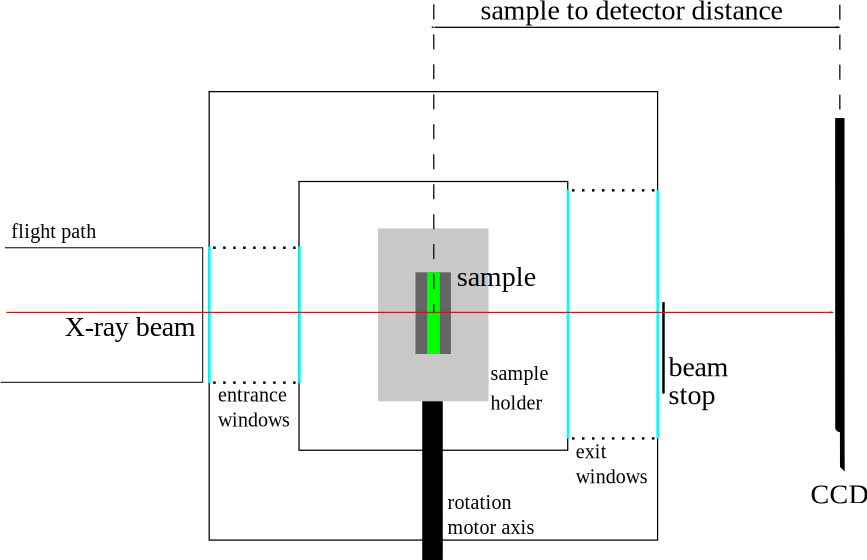
\includegraphics[width=0.85\textwidth]{figures/Tat/MMs/chamber_geometry}
  \caption[Schematic diagram of a top view of the X-ray setup for LAXS experiments]
  {Schematic diagram of a top view of the X-ray setup for LAXS experiments.
  A green lipid sample deposited on a dark gray Si wafer 
  was situated on top of a Peltier cooling/heating
  device, which was attached to the light gray sample holder. 
  The sample holder was mounted on the black rotation motor axis, which provided 
  precise control of the incident angle $\omega$. Thin mylar windows shown 
  in cyan allowed incoming
  and outgoing X-rays shown as a red arrow to go through the chamber.
  Thin pieces of molybdenum attenuated
  the direct beam to avoid saturation of CCD pixels and conveniently allowed 
  beam profile measurements due to its transparency. The flightpath and hydration chamber
  were filled with helium to reduce air scattering.}
  \label{fig:x-ray_setup}
\end{figure}

%%%%%%%%%%%%%%%%%%%%%%%%%%%%%%%%%%%%%%%%%%%%%%%%%%%%%%%%%%%%%%%%%%%%%%%%%%%%%%%
\subsection{Analysis of Diffuse Scattering}\label{sec:diffuse_analysis}
Figure~\ref{fig:figure1} shows our typical LAXS data 
from oriented stacks of fluctuating bilayers in the fluid phase. 
The analysis of diffuse scattering 
intensity patterns like the one shown in Fig.~\ref{fig:figure1} yields material 
parameters such as the bending modulus \gls{Kc} and bulk modulus \gls{B} as well as
the absolute form factor $|F(q_z)|$. 
The X-ray form factor \gls{Fq} is the Fourier transform of the bilayer electron 
density profile \gls{rhoz} normal to the membrane plane 
and is related to the internal structure of the
bilayers including Tat peptides.

\begin{figure}[htbp]
  \centering
  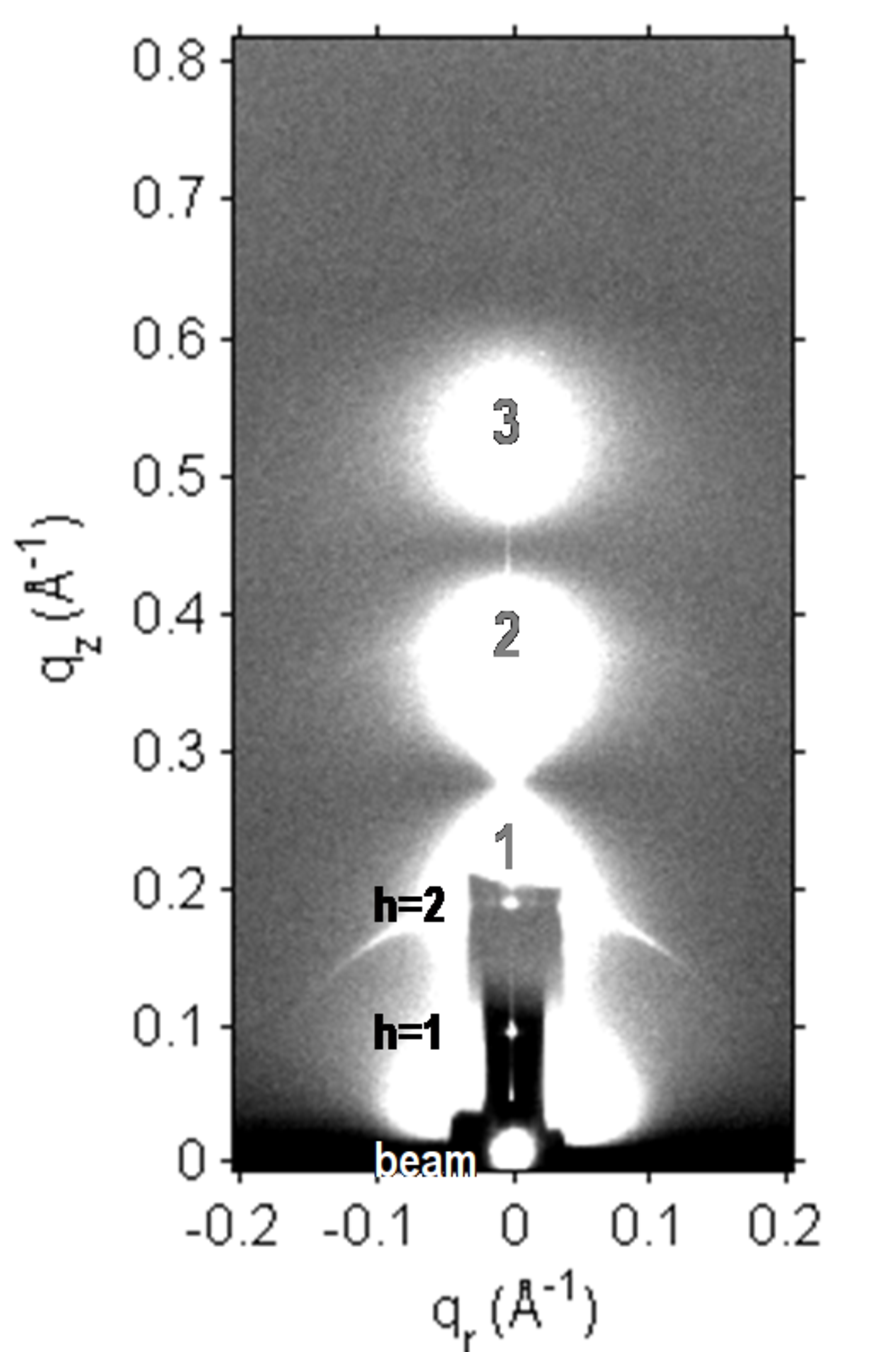
\includegraphics[width=0.5\textwidth]{figures/Tat/NFIT_results/dopcdope1to1}
  \caption[LAXS of DOPC:DOPE (1:1) with $\xTat$ = 0.034 at 37 \textcelsius]
  {LAXS of DOPC:DOPE (1:1) with $\xTat$ = 0.034 at 37 \textcelsius. 
  White lobes of diffuse scattering intensity have large grey numbers, while
  lamellar orders and beam are shown to the left of the
  molybdenum beam attenuator (short, dark rectangle). $q_z$ and $q_r$ are the 
  cylindrical coordinates of the sample $q$-space, where the $q_z$-axis is along 
  the bilayer normal and the $q_r$-axis is along the in-plane direction. 
  The lamellar repeat spacing was $D$ = 66.2 \AA.}
  \label{fig:figure1}
\end{figure}

The form factor $|F(q_z)|$ is obtained through the relation
$I(\mathbf{q})= S(\mathbf{q})|F(q_z)|^2$, where \gls{Iq} is the measured intensity,
and \gls{Sq} is the structure factor.
Here, \gls{q} = (\gls{qr},~\gls{qz}), indicating that the system is isotropic in-plane. 
In fully hydrated multilamellar samples, $S(\mathbf{q})$ is not a sum of delta 
functions because of thermal fluctuations of bilayers. Calculating $S(\mathbf{q})$
requires a model free energy for bilayer fluctuations, from which the scattering
pair correlation function is derived. A basic scattering theory, then, relates
the scattering intensity $I(\mathbf{q})$ to the pair correlation function. 
For modeling the membrane fluctuations of a multilamellar system, 
the smectic liquid crystal free energy functional in the discrete form,
\begin{equation}
  F=\frac{1}{2}\int d\mathbf{r}\sum _{n=0}^{N-1}\left\{ 
  K_{c} \left[\nabla _{r}^{2}u_{n}\left(\mathbf{r}\right)\right]^{2}
  +B\left[u_{n+1}\left(\mathbf{r}\right)-u_{n}\left(\mathbf{r}\right)\right]^{2}
  \right\},
  \label{eq:free_energy}
\end{equation}
has been shown to be adequate \cite{Lyatskaya01}.
Here, $u_{n}\left(\mathbf{r}\right)$ is the spatial deviation of the center 
of the $n$-th bilayer from its average position in the $z$ direction
at the in-plane location $\mathbf{r}=(x,y)$ (Fig.~\ref{fig:stack}).
The first term is the bending free energy proportional to the curvature
squared with the proportionality given by a bending modulus $K_{c}$, and
the second term is a harmonic approximation to the interactions between
membranes with a modulus $B$. 
Once $S(\mathbf{q})$ is calculated 
from Eq.~(\ref{eq:free_energy}), $|F(q_z)|$ can 
be calculated by dividing the intensity by $S(\mathbf{q})$. 
Getting the best fit of a model $S(\mathbf{q})$ to the intensity results in 
the material parameters, $K_c$ and $B$.

\begin{figure}[htbp]
  \centering
  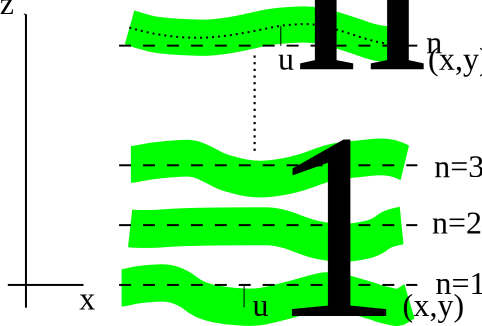
\includegraphics[width=0.5\textwidth]{figures/Tat/MMs/stack}
  \caption[Schematic of an oriented stack of lipid bilayers]
  {Schematic of an oriented stack of lipid bilayers. Thick green curves
  represent an instance of thermally fluctuating bilayers. The dashed lines 
  show the thermally averaged positions $z=nD$ of the centers of each bilayer 
  and $u_{n}(x,y)$ gives the instantaneous deviation from the average. 
  Each bilayer extends in the $\mathbf{r}=\left(x,y\right)$ plane.}
  \label{fig:stack}
\end{figure}

We used software called NFIT developed by Dr. Yufeng Liu
\cite{Lyatskaya01,Liu04,Liu03} to analyze the diffuse scattering and
obtain $K_c$, $B$, and $|F(q_z)|$. 
Details of the analysis, including the theoretical derivation of
$S(\mathbf{q})$ from Eq.~(\ref{eq:free_energy}) and its
numerical computation, are found in Liu's thesis 
\cite{Liu03}. 

%%%%%%%%%%%%%%%%%%%%%%%%%%%%%%%%%%%%%%%%%%%%%%%%%%%%%%%%%%%%%%%%%%%%%%%%%%%%%%%
\subsection{Modeling the Bilayer Structure}\label{sec:SDP_method}
The simplest way to represent the results of X-ray data in real space is to 
Fourier transform the $F(q_z)$ form factors to obtain electron density profiles 
$\rho(z)$. However, the $\rho(z)$ so obtained are on an arbitrary scale.  
Furthermore, no information is obtained regarding the location of component 
groups of the lipid or the location of added peptides.  
Finally, Fourier reconstruction requires knowing the phase factors of individual 
reflections; this latter concern is alleviated when diffuse scattering is 
obtained as the zeros in $I(q_z)$ locate where the phase factors change sign.  
Modeling uses the intensities, not the phase factors, obtains absolute electron densities, and 
estimates where the different components of the system are located.  
Early so-called strip models used constant $\rho(z)$ in different $z$ regions
\cite{King86}.  
This has been improved by using error functions to smear the artificially sharp 
edges of the strip model \cite{Heinrich14,Shekhar11}. 
When the width of two error function interfaces are wide compared to the distances 
between the edges, the profile becomes a Gaussian.  
Models consisting of sums of Gaussians have been used \cite{Mitsui78}.  
A hybrid model used positive Gaussians for the headgroup and a negative Gaussian 
for the terminal methyl region superimposed on a modulated baseline for the water 
and the hydrocarbon \cite{ref:Wiener89}, which was later replaced by 
error functions for the hydrocarbons and for water \cite{Klauda06}.  
This lab now uses the SDP method which imposes a volumetric constraint to account 
for the water profile \cite{Kucerka08}.  

The SDP method is applicable to joint fitting of neutron and X-ray scattering data 
when a particular parsing of the component groups is employed.  
For X-ray scattering data alone, a different parsing is more appropriate.  
The parsing of DOPC into molecular components is shown in
Fig.~\ref{fig:dopc_schematic}. The phosphate/choline (PC) and 
carbonyl/glycerol (CG) components together make up the lipid headgroup
whereas the hydrocarbon chain region (HC)
is divided into two components, the methylene (CH$_2$) and methine (CH) group
combination (denoted as CH$_2$+CH) and terminal methyl groups (CH$_3$). 
We combine methylene (CH$_2$) and methine groups (CH) in order to 
minimize the number of fitting parameters.

\begin{figure}[htbp]
  \centering
  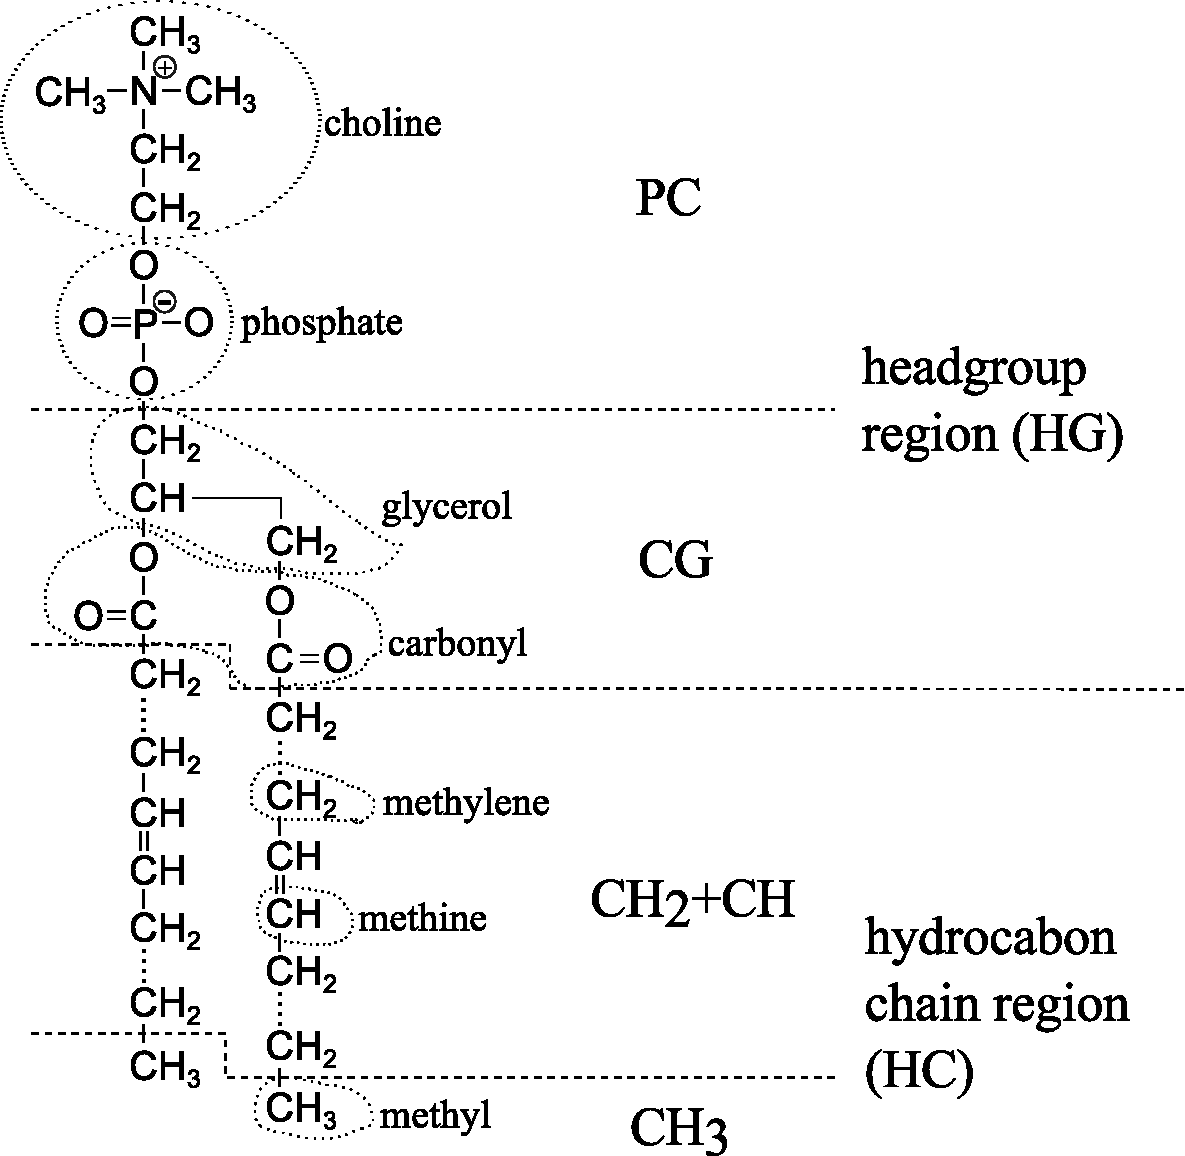
\includegraphics[width=0.9\textwidth]{figures/Tat/MMs/dopc_schematic.pdf}
  \caption[Schematic of DOPC showing each molecular component]
  {Schematic of DOPC showing each molecular component. The dashed lines 
  show where the lipid is divided into different components. 
  The lipid headgroup
  is divided into two components, phosphate-choline (PC) and carbonyl-glycerol (CG). 
  The hydrocarbon chain region is also divided
  into two components, methylene+methine (CH$_2$+CH) and terminal methyl groups (CH$_3$).
  Each hydrocarbon chain has 18 carbons. Repeated methylene groups 
  are shown by dots.}
  \label{fig:dopc_schematic}
\end{figure}

\subsubsection{Functional Forms}
Our model for the electron density profile (EDP)
of the Tat/lipid bilayer system consists of five structural subgroups: PC, CG,
CH$_2$+CH, CH$_3$, and Tat (see Fig.~\ref{fig:DOPC_EDP}).
Assuming bilayers are centrosymmetric, 
the volume probability distributions of components PC, CG, CH$_3$, and Tat 
are described by Gaussian functions,
\begin{equation}
  P_i(z)=\frac{c_i}{\sqrt{2\pi}}\pars{
    \exp\braces{-\frac{(z+z_i)^2}{2\sigma_i^2}}
	+ \exp\braces{-\frac{z-z_i)^2}{2\sigma_i^2}}
  },
\end{equation}
where $i$ specifies a particular molecular component,
PC, CG, Tat, CH+CH$_2$, and CH$_3$, and
$c_i$ is an integrated area underneath the curve and the two parts of the 
expression describe the two bilayer leaflets. 

\begin{figure}[htbp]
  \centering
  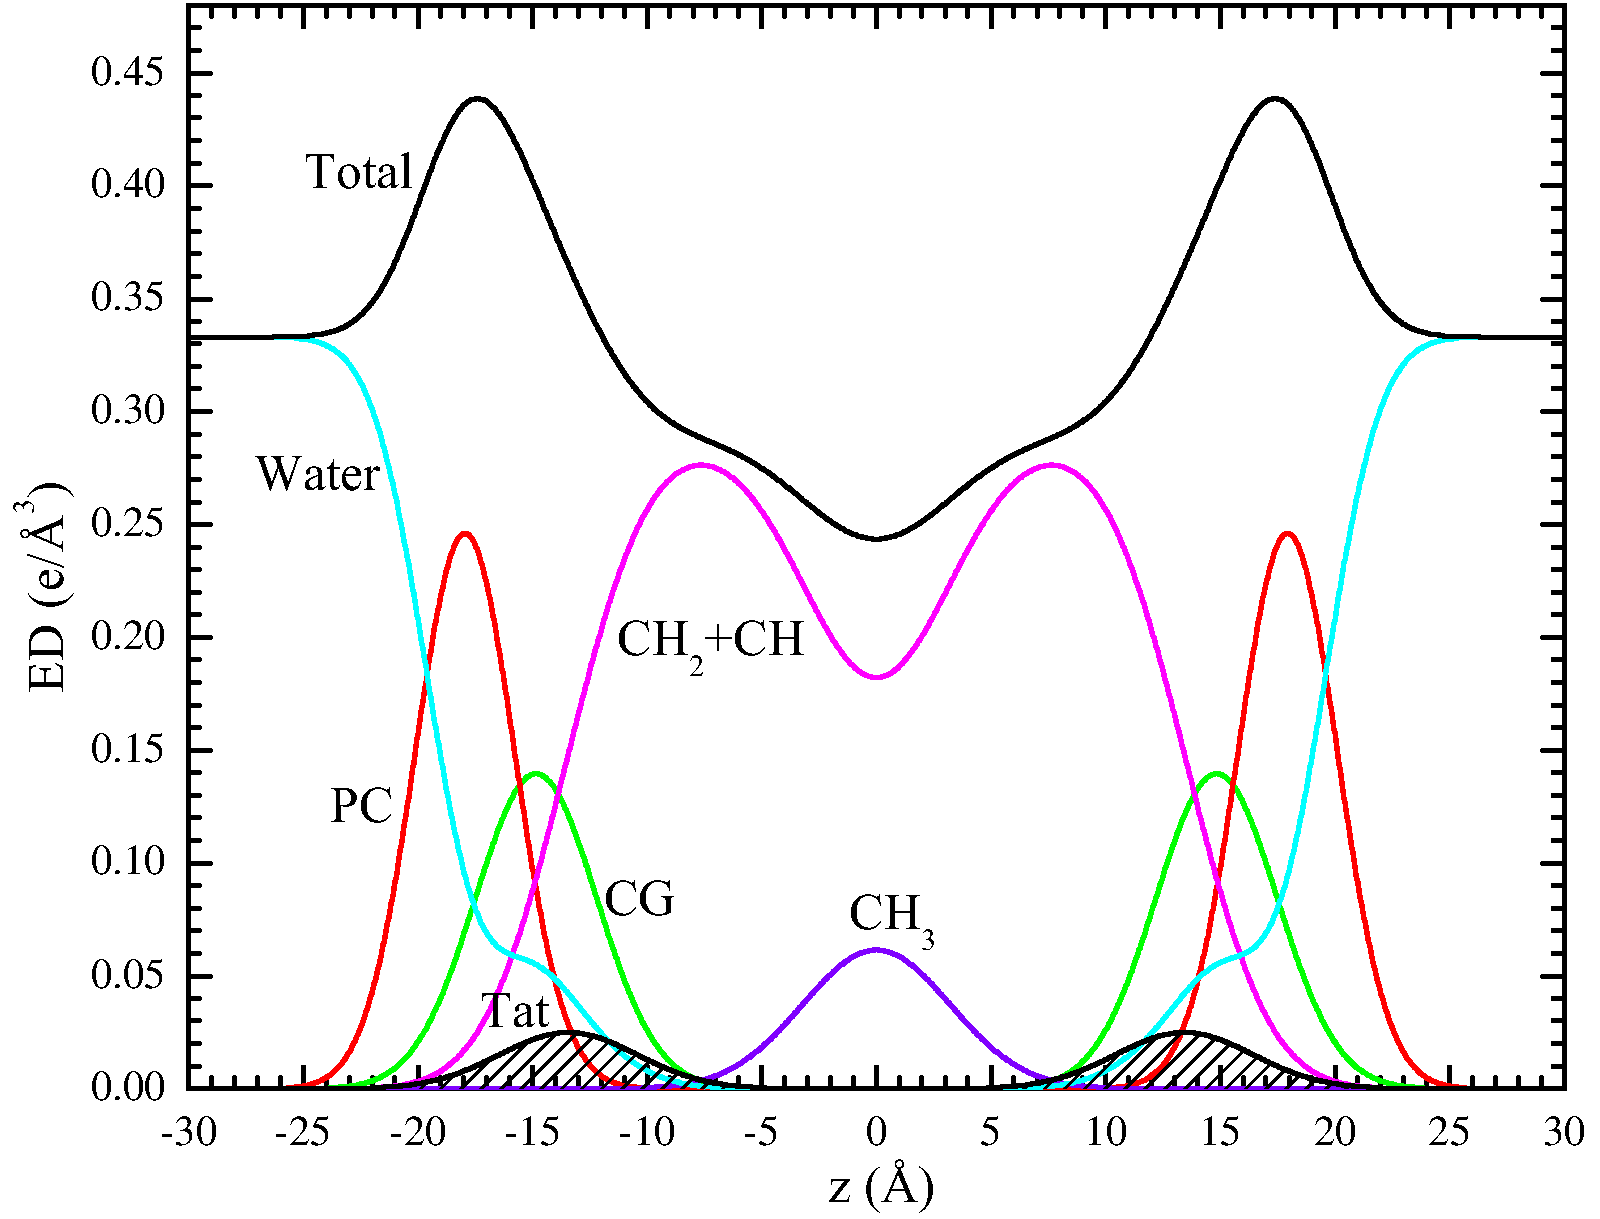
\includegraphics[width=0.9\textwidth]{figures/Tat/SDP_Results/EDP/DOPC_Tat_model_EDP}
  \caption[A model electron density profile for DOPC with Tat]
  {A model electron density profile for DOPC with Tat. Lipid components
  are defined in Fig.~\ref{fig:dopc_schematic}. Tat profile is the black shaded
  curve. The black solid line labelled `Total' is the sum of all components.}
  \label{fig:DOPC_EDP}
\end{figure}

The hydrocarbon chain region (HC) is represented by error functions,
\begin{equation}
  \PHC(z) = \frac{1}{2}\bracks{
    \mathrm{erf}(z,-\z{HC},\sigmaHC) - \mathrm{erf}(z,\z{HC},\sigmaHC)
  },
\end{equation}
where
\begin{equation}
  \mathrm{erf}(z,z_i,\sigma_i)=\frac{2}{\sqrt{\pi}}
    \int_0^{\frac{z-z_i}{\sqrt{2\sigma}}} \dx e^{-x^2}.
\end{equation}
The volume probability distribution for the methylene and methine group
combination can then be expressed as
\begin{equation}
  \PCHtwoCH(z) = \PHC(z)-\PCHthree(z).
  \label{eq:modelA}
\end{equation}
This definition enforces the total probability $\PHC$ in the hydrocarbon
chain region to equal one, which in turn means that placement of Tat in the  
chain region is prohibited. We call the model defined by Eq.~(\ref{eq:modelA})
Tat-in-headgroup (THG). To allow Tat to be placed inside the hydrocarbon
chain region, we also consider an alternative definition,
\begin{equation}
  \PCHtwoCH(z) = \PHC(z)-\PCHthree(z) - \PTat(z),
\end{equation}
where the volume probability of the CH$_2$+CH combined component is reduced by 
the Tat volume probability distribution. We call this model Tat-in-hydrocarbon-chain (THC).
The spatial conservation requires the water volume probability distribution 
to be
\begin{equation}
  \PW(z) = 1-\PPC(z)-\PCG(z)-\PTat(z)-\PHC(z)
\end{equation}
for THG and
\begin{equation}
  \PW(z) = 1-\PPC(z)-\PCG(z)-\PHC(z)
\end{equation}
for THC. 

Because X-rays measure the contrast between the bilayer and surrounding solvent, 
the experimental form factor is compared to the water subtracted model
form factor,
\begin{equation}
  F(q_z) = 2\int_0^{\frac{D}{2}} \dz \pars{
    \sum_i(\rho_i-\rhoW)P_i(z)
  } \cos(q_zz),
\end{equation}
where $i$ = PC, CG, Tat, CH+CH$_2$, and CH$_3$.

%%%%%%%%%%%%%%%%%%%%%%%%%%%%%%%%%%%%%%%%%%%%%%%%%%%%%%%%%%%%%%%%%%%%%%%%%%%%%%%
\subsubsection{Constraints}
The height of the hydrocarbon chain error function is fixed to one by imposing
spatial conservation, whereas the mean position of the terminal methyls is
fixed to $\zCHthree=0$ by symmetry arguments. The total lipid volume
$\VL$ is fixed to the experimentally measured value. 
The headgroup volume $\VHL$ was determined to be 331 \AA$^3$ for 
gel phase phosphatidylcholine (PC) bilayers \cite{Tristram-Nagle02},
and we assume the same volume for the fluid phase PC bilayers.
The volumes of PC and CG components satisfy
\begin{equation}
  \VPC + \VCG = \VHL,
\end{equation}
and the volumes of CH$_3$ and CH$_2$+CH components satisfy
\begin{equation}
  2\left(16\VCHtwoCH + \VCHthree\right) = \VL-\VHL.
\end{equation}
These component volumes constrain the heights of the Gaussians as
\begin{align}
  \cPC &= \frac{\VPC}{\AL\sigmaPC} \\
  \cCG &= \frac{\VCG}{\AL\sigmaCG} \\
  \cCHthree &= \frac{2\VCHthree}{\AL\sigmaCHthree} \\
  \cTat &= \frac{\VTat}{\AL\sigmaTat}
\end{align}
where $\AL$ is area per lipid.

The ratio of 
the carbonyl/glycerol volume to the headgroup volume $\VHL$ was
reported to be 0.41 \cite{Braun13}, so we constrain the CG
component volume to 135.7 \AA$^3$ and the PC component volume to 
195.3 \AA$^3$. 

The most detailed structural study on DOPC to date was published 
by Braun \textit{et al.} \cite{Braun13}, 
and many of the constraints on our model parameters can be derived
from their study. However, in that work, the authors used the 
SDP model \cite{Kucerka08}, which is specifically tailored for
simultaneous analysis of neutron and X-ray form factors. 
Therefore, we need to convert their structural results to the 
corresponding parameters in our simpler X-ray model. For example, 
from the reported values of the ratio of the volumes of the chain terminal
methyl (CH$_3$) to the chain methylenes (CH$_2$) and the ratio of 
the volumes of the chain methines (CH) to the chain methylenes, we can
calculate the ratio $\rCHthree$ of the volumes of CH$_3$ to the CH$_2$ and
CH combined component.  
Furthermore, the study by Braun \textit{et al.} was at 30 \textcelsius\
while our study was at 37 \textcelsius, so our
measured volume of DOPC was slightly greater.

At 30 \textcelsius, the volume of DOPC was reported to be 1303 \AA$^3$ \cite{Kucerka08}, 
so the volume of hydrocarbon chain region at the same temperature is 
$1303 - 331 = 972$ \AA$^3$. The ratio $r$ of the volumes
of the chain terminal methyl (CH$_3$) to the chain methylenes (CH$_2$) was 
reported to be 1.95, and the ratio $r_{12}$ of the volumes of the chain
methines (CH) to the chain methylenes was 0.91 at 30 \textcelsius. 
Because there are 14 CH$_2$ groups,
2 CH groups, and 1 CH$_3$ group in each DOPC hydrocarbon chain, we have
$2\times(14\VCHtwo+2\VCH+\VCHthree)=972$ \AA$^3$. 
Using $r=\VCHthree/\VCHtwo=1.95$ 
and $r_{12}=\VCH/\VCHtwo=0.91$, we get $\VCHtwo=27.3$ \AA$^3$, 
$\VCH=24.9$ \AA$^3$, and $\VCHthree=53.3$ \AA$^3$. 
These calculated volumes lead to $\VCHthree/\VCHtwoCH=1.97$  for 30 \textcelsius. 

At 37 \textcelsius, the volume of DOPC was measured to be 1313.5 \AA$^3$, so
we have $2\times(16\VCHtwoCH+\VCHthree)=1313.5-331$. Assuming that the ratio 
$\VCHthree/\VCHtwoCH$ at 37 \textcelsius\ is the same as that at 30 \textcelsius\ 
gives $\VCHtwoCH=27.3$ \AA$^3$ and $\VCHthree=53.9$ \AA$^3$. We constrain
the components for the hydrocarbon chain region in our model 
to these calculated values.

\begin{table}[htbp]
  \centering
  \begin{tabular}{ccc}
    \hline
    lipid & number of electrons & volume (\AA$^3$) \\
    \hline
    DOPC & 434 & 1313.5 \\
    DOPE & 410 & 1212.3 \\
    DOPC:DOPE (3:1) & 428 & 1288.2 \\
    \hline
  \end{tabular}
  \caption[Number of electrons and volume per lipid]
  {Number of electrons and volume per lipid.}
  \label{tab:electron_volume}
\end{table}

\begin{table}[htbp]
  \centering
  \begin{tabular}{cccc}
    \hline
    component & $n^e_i$ & $V_i$ (\AA$^3$) & $\rho_i$ (e/\AA$^3$) \\
    \hline 
    PC & 97 & 195.3 & 0.497 \\  
    PE & 73 & 94.1  & 0.776 \\
    PC:PE (3:1) & 91 & 170 & 0.535 \\
    CG & 67 & 135.7 & 0.494 \\  
    CH$_2$+CH & 7.875 & 27.3 & 0.288 \\
    CH$_3$ & 9 & 53.9 & 0.167 \\
    \hline
  \end{tabular}
  \caption[Structural parameters for each component]
  {Structural parameters for each component.   $n^e_i$ is the number of 
  electrons and $\rho_i$ is the average electron density. $V_i$ is the 
  molecular volume.}
  \label{tab:component}
\end{table}

\begin{table}[htbp]
  \centering
  \begin{tabular}{c c c}
    \hline
    number of electrons & 838 \\ 
    volume (\AA$^3$) & 1877 \\
    $\rho_\textrm{Tat}$ (e/\AA$^3$) & 0.446 \\
    \hline
  \end{tabular}
  \quad
  \begin{tabular}{ ccc }
    \hline
    mole fraction ($\xTat$) & $n^e_\textrm{Tat}$ & $\VTat$ (\AA$^3$) \\    
    \hline
    0.016 & 13.6 & 30.5 \\
    0.034 & 29.5 & 66.1 \\
    0.059 & 53.0 & 118.8 \\
    \hline
  \end{tabular}
  \caption[Tat basic structural parameters]
  {Tat basic structural parameters. The notations are the same
  as in Table~\ref{tab:component}. $\xTat$ is Tat mole fraction.}
  \label{tab:Tat_basic_params}
\end{table}

%\begin{table}[htbp]
%  \centering
%  \begin{tabular}{c c c c c c c c}
%    \hline
%     & DOPC & \multicolumn{2}{c|}{62:1} & \multicolumn{2}{c|}{28:1} & \multicolumn{2}{c|}{16:1} \\
%    \cline{3-8}
%     & & A & B & A & B & A & B \\
%    \hline
%    $\VL$ & 1314 & 1344 & 1344 & 1380 & 1380 & 1432 & 1432 \\    
%    $\VHL$ & 331 & 362 & 331 & 397 & 331 & 450 & 331 \\  
%    $\VTat$ & 0 & 30.5 & 30.5 & 66.1 & 66.1 & 119 & 119 \\  
%    $\RPC$ & 0.59 & 0.54 & 0.59 & 0.49 & 0.59 & 0.43 & 0.59 \\
%    $\RCG$ & 0.41 & 0.38 & 0.41 & 0.34 & 0.41 & 0.30 & 0.41 \\
%    $\RTat$ & 0   & 0.08 & 0    & 0.17 & 0    & 0.27 & 0 \\ 
%    $r_{12}$ & 0 & 0 & 0.558 & 0 & 1.21 & 0 & 2.17 \\
%    $r$ & 1.97 & 1.97 & 1.97 & 1.97 & 1.97 & 1.97 & 1.97 \\ 
%    \hline
%  \end{tabular}
%  \caption{Volumetric constraints. A and B refer to two different models 
%  described in the text.}
%  \label{tab:model_constraints}
%\end{table}
%------------------------------------------------------------------------------

%%%%%%%%%%%%%%%%%%%%%%%%%%%%%%%%%%%%%%%%%%%%%%%%%%%%%%%%%%%%%%%%%%%%%%%%%%%%%%%
\subsubsection{Fits with Lower Bounds}
Modeling of the bilayer structure was done using the SDP software, 
as described in Sec.~\ref{sec:SDP_method}.
To allow model parameters with upper and lower bounds, the
SDP software was modified following the MINUIT User's Guide, section 1.3 
\cite{minuit}. 
Briefly, the modified minimization routine ``sees'' internal variables 
at each iteration. These internal variables can take on
any values between $-\infty$ to $+\infty$, which is an assumption made
in a typical minimization routine such as 
the simplex method and Levenburg-Marquadt algorithm.
A model parameter with both lower and upper bounds ($a$ and $b$, respectively) 
is related to its corresponding internal variable by the following transformation,
\begin{align}
  P_\textrm{int} &= \arcsin \pars{2\frac{P_\textrm{ext}-a}{b-a}-1}  \\
  P_\textrm{ext} &= a + \frac{b-a}{2}(\sin P_\textrm{int}+1),
  \label{eq:internal_external}
\end{align}
where $P_\text{int}$ is the value of an internal variable and
$P_\text{ext}$ is the value of a model parameter. It is easy to show that
$P_\text{ext}$ can only take values between $a$ and $b$.
The goodness of a fit $\chi^2$ is then calculated by transforming the
internal variables to their respective model parameters via Eq.~(\ref{eq:internal_external}). 
For variables with a lower bound $a$ only, the transformation is
\begin{align}
  P_\textrm{int} &= \sqrt{(P_\textrm{ext}-a+1)^2 - 1} \\
  P_\textrm{ext} &= a - 1 + \sqrt{P_\textrm{int}^2+1}, 
\end{align}
and for variables with an upper bound $b$ only,
\begin{align}
  P_\textrm{int} &= \sqrt{(b-P_\textrm{ext}+1)^2 - 1} \\
  P_\textrm{ext} &= b + 1 - \sqrt{P_\textrm{int}^2+1}.
\end{align}
This nonlinear transformation between internal variables and model parameters 
allowed model parameters with upper and lower bounds in
the SDP program.

%%%%%%%%%%%%%%%%%%%%%%%%%%%%%%%%%%%%%%%%%%%%%%%%%%%%%%%%%%%%%%%%%%%%%%%%%%%%%%%
\newpage
\subsection{Molecular Dynamics Simulation}\label{sec:sim_methods}
This section describes the MD simulations performed by Dr. Kun Huang, who was
a graduate student of Prof. Angel Garcia at Rensselaer Polytechnic Institute
when he collaborated with the Nagle/Tristram-Nagle lab.
My contribution to the MD simulations was to help analyze the results.

Systems with different DOPC/Tat mole ratios (128:0, 128:2 and 128:4, corresponding to
0, 0.015, and 0.030 mole fractions) were simulated atomistically using the Gromacs 4.6.1
package \cite{Hess08}. 
DOPC was modeled by the Slipid force field 
\cite{Jambeck12_JPCB,Jambeck12_JCTC},
and HIV-1 Tat was modeled by Amber 99SB \cite{Hornak06}. 
Tip3p water was used \cite{Jorgensen83}. The number of Tats was divided equally on
each side of the bilayer to mimic experimental conditions. All systems were simulated at 310 K
with a constant area in the $x$-$y$ plane and 1 atm constant pressure in the $z$ direction. Each
system was simulated for 100 ns, and the last 50 ns was used as the production run.
At each DOPC/Tat mole ratio, we studied systems with three different area/lipid ($\AL$).
For the DOPC system, we fixed $\AL$ = 68, 70, 72 \AA$^2$; 
DOPC/Tat (128:2), we fixed $\AL$ = 72, 74, 76 \AA$^2$; 
DOPC/Tat (128:4), we fixed $\AL$ = 72, 74, 76 \AA$^2$. 
These areal values were based on the analysis of experimentally obtained form 
factors, which is discussed in Sec.~\ref{sec:SDP_results}.
For systems with Tat, chloride ions were used as counterions.
For each DOPC/Tat system at fixed $\AL$, 
we then conducted seven independent simulations with the center of mass (COM) of
each Tat constrained at different distances from the bilayer center 
(18, 16, 14, 12, 10, 8, and 5 \AA). 
In total, 45 independent simulations were conducted. 
The goal of the constrained simulations was to find the best match between 
experimental and MD simulation form factors. Comparison to
the X-ray form factors was performed using the SIMtoEXP software 
written by Dr. Norbert Ku\v{c}erka \cite{Kucerka10}. 

All simulations were conducted with a 2 fs time integration step. 
SETTLE \cite{Miyamoto92} was used
to constrain water molecules, and LINCS \cite{Hess97} was used to constrain all other bond lengths in the
system. 
Van der Waals interactions were truncated at 1.4 nm with a twin-range cutoff scheme and a
dispersion correction was applied to both energy and pressure. Electrostatic interactions were
treated with the particle-mesh Ewald (PME) method \cite{Darden93}. The direct term for electrostatics was
evaluated within 1.0 nm cutoff and the Fourier term was evaluated with a 0.12 nm grid spacing
and a 4th order interpolation. Each system was simulated at 310 K using the V-rescale
algorithm \cite{Bussi07} with a 0.2 ps time coupling constant. The semi-isotropic parrinello-rahman barostat
\cite{Parrinello81} was used to couple the system at 1 atm in the $z$ direction with a 5 ps time coupling constant,
while the projected area at the $x-y$ plane was fixed by setting the system compressibility to 0.
We inserted the Tats into the system by initially turning off all interactions between Tats and the
rest of the system, with Tats constrained at different depths. Then we slowly turned on the
interactions to normal strength through thermodynamics integrations. We used umbrella
potentials to constrain Tats at desired depths with a force constant of 3000 kJ/mol/nm$^2$.

The center of mass (COM) distance between each peptide and the bilayer was 
constrained by an umbrella potential. 
Essentially, this potential acts as a spring, 
where its potential energy depends on the deviation of the distance 
between the center of mass of Tat and DOPC from a preferred value, $z_0$,
\begin{equation*}
  U(z_1^{\textrm{Tat}},\ldots,z_1^{\textrm{DOPC}},\ldots) = 
  -\frac{1}{2} k 
  \pars{z_{\textrm{cm}}^{\textrm{Tat}} - z_{\textrm{cm}}^{\textrm{DOPC}} - z_0}^2.
\end{equation*}
Then, $-\partial U/\partial z_i$ is the external force acting 
on atom, $i$. 

%%%%%%%%%%%%%%%%%%%%%%%%%%%%%%%%%%%%%%%%%%%%%%%%%%%%%%%%%%%%%%%%%%%%%%%%%%%%%%%
\section{Analysis of Molecular Dynamics Simulation Data}
\subsection{SIMtoEXP Program}\label{sec:SIMtoEXP}
This section briefly describes the SIMtoEXP program
developed by Ku\v{c}erka \textit{et al.} \cite{Kucerka10}.
Essentially, for each snapshot, the positional distribution of each atom
averaged over the $xy$ plane is calculated. Then, the distribution is
averaged over snapshots. The product of this distribution and the average
electron density gives the electron density profile of the atom. The sum 
over all the electrons provides the total electron density profile. This total
electron density profile minus the average electron density of water
is Fourier transformed to provide the X-ray form factor.
\begin{equation}
  F^\textrm{sim}(q_z) = \int_0^\infty\dz (\rho(z)-\rhoW)\cos (q_zz).
\end{equation}
Simulated electron density profiles were symmetrized, and then
$F^\textrm{sim}(q_z)$ was calculated with $\rhoW$ = 0.326 e/\AA$^3$,
which was the average electron density of water molecules in the MD simulations.
Because $\rho(z)$ is equal to $\rhoW$ outside the bilayer, the upper 
integration limit can be truncated to a finite value. 

Because the experimental form factor is in arbitrary units, it is 
scaled by a single constant $a$ to produce the best fit to the simulated
form factor through a linear least squares fit that minimizes the 
following goodness of fit
\begin{equation}
  \chi^2 = \sum_i \left(\frac{1}{\sigma_i}\pars{
    a|F^\textrm{exp}_i| - |F^\textrm{sim}(q_{z,i})|
  }\right)^2
  \label{eq:SIMtoEXP}
\end{equation}
where $\sigma_i$ is the input experimental uncertainty and $F_i^\textrm{exp}$
is the experimental form factor measured at $q_z = q_{z,i}$.
\gls{chisqr} defined by Eq.~(\ref{eq:SIMtoEXP}) does not keep the relative errors
$\sigma_i$/$|F_i^\textrm{exp}|$ constant. 
To properly calculate the goodness of a fit, relative errors must be 
independent of an overall scaling factor $a$, so
the $\chi^2$ values calculated by the program were multiplied by 1/$a^2$. 
These corrected $\chi^2$ values are reported in this chapter.

%%%%%%%%%%%%%%%%%%%%%%%%%%%%%%%%%%%%%%%%%%%%%%%%%%%%%%%%%%%%%%%%%%%%%%%%%%%%%%%
\subsection{Local Thinning of Membranes}\label{sec:local_thinning}
The SIMtoEXP program gives the average quantities for each leaflet. 
Our X-ray data are only sensitive to the average bilayer electron density;
in contrast, local information concerning Tat-bilayer interactions can be obtained from MD simulations.
In this section, we discuss a method to extract a local membrane thickness
around the Tat peptides from the MD simulation trajectories. 

One of the expected effects of Tat interacting with a bilayer is 
compression of the lipid bilayer along the $z$-direction. It is 
reasonable to assume that this compression is greater near Tat and
weaker far from Tat.
Then, the distance \gls{Dphos} between phosphorus atoms in opposite
leaflets near Tat should be different from the distance between
phosphorus atoms away from Tat.  
For a small Tat concentration, $\Dphos$ is the same as that of 
pure DOPC if the distance from all Tats is large enough.  
For our experimental concentrations, the thinning effect may extend throughout 
the bilayer because the lateral effect of Tat might have a larger lateral decay 
length than the distance between Tats. Whether that is the case or not, we 
expect that the bilayer thickness near a Tat is smaller than the average thickness,
so $\Dphos$ should represent the actual thinning effect due to Tat. 

\begin{figure}[htbp]
  \centering
  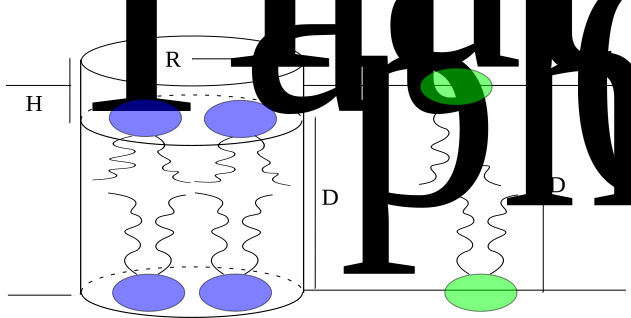
\includegraphics[scale=0.7]{./figures/Tat/MMs/cylinder_model}
  \caption[Our simple model to extract the local bilayer thickness from 
  simulation trajectories]
  {Our simple model to extract the local bilayer thickness from 
  simulation trajectories. Tat is modeled as a cylinder with height $\HTat$ 
  and radius $\RTat$. The local bilayer thickness is defined as $\Dphos$. 
  The thickness of the unperturbed DOPC bilayer is $\Dphos^0$. 
  Lipids with blue headgroups fall within the imaginary cylinder extended from
  Tat. Unperturbed lipids have green headgroups.}
  \label{fig:cylinder_model}
\end{figure}
 
First, let us define what we mean by lipids close to Tat.  
As in Fig.~\ref{fig:cylinder_model}, we imagine a cylinder around Tat and 
find all the phosphorus atoms within it. 
Approximating Tat as a cylinder 
with its height \gls{HTat} given by the FWHM of simulated electron density distribution, 
its radius \gls{RTat} is calculated from the experimentally determined volume $\VTat$ = 1876 \AA$^3$ 
using $\RTat=\sqrt{\VTat/(\pi\HTat)}$. 
Let us define the lateral center of the cylinder as the center of mass of each
Tat. Then we define $\Dphos$ using only those lipids whose 
phosphorus atoms lie within these $\RTat$ cylinders around a Tat. 
Then $\Dphos= \zphos^+ - \zphos^-$ where $\zphos^+$ and $\zphos^-$ 
are the average $z$ of the $n^+$ ($n^-$) lipids in the upper and lower monolayer, respectively.  

The algorithm for doing the above was straightforward.  
For each time frame, the positions ($x_i$, $y_i$, $z_i$) of each Tat, $i$, are 
listed.   
We chose phosphorus atoms whose ($x$, $y$) lateral position lay within 
$\RTat$ of any Tat position. Then, $z$ positions
of the chosen phosphorus atoms were placed in a list, from which
\gls{zphos} was calculated. 
Dr. Huang supplied us with files containing the value of $\zphos$ 
at each snapshot, and I wrote a script to average over many snapshots 
to improve statistics. 

%%%%%%%%%%%%%%%%%%%%%%%%%%%%%%%%%%%%%%%%%%%%%%%%%%%%%%%%%%%%%%%%%%%%%%%%%%%%%%%
\subsection{Lateral Decay Length of Membrane Thinning}\label{sec:lateral_decay}
This section describes a method to measure the lateral decay length
of membrane thinning due to Tat-lipid interactions. 
As in the previous section, Tat is modeled as a cylinder with 
its radius equal to $\RTat$, height $\HTat$,
and volume $\VTat$ such that $\RTat=\sqrt{\VTat/(\pi \HTat)}$. 
Let $h(r)$ represent the phosphorus height profile
of a leaflet as in Fig.~\ref{fig:linear_model}. The two leaflets are assumed to be decoupled.
In our model, lipids are separated into three regions: 
suppressed, boundary, and unperturbed region. 
The suppressed region extends from $r=0$ to $\RTat$ and is directly beneath 
(above) Tat in the top (bottom) leaflet. In this region, lipids are uniformly 
compressed by Tat toward the 
center of the bilayer, so that $h(r)$ is a constant equal to $\zphos$. 
From $r=\RTat$ to $R_2$ is the boundary region, where $h(r)$ is assumed to 
linearly increase with the lateral distance $r$. The lateral decay length
of membrane thinning is given by $R_2$. 
In the unperturbed region ($r>R_2$), lipids do not interact with 
Tat, behaving identically to DOPC, so the phosphorus position is the same as that of 
DOPC. A continuous $h(r)$ that 
satisfies the above criteria is
\begin{equation}
  h(r) = \left\{ 
  \begin{array}{lcr}
    \zphos   & \text{if} & 0   \leq r < \RTat \\
    mr+b     & \text{if} & \RTat \leq r < R_2 \\
    \zphos^0 & \text{if} & R_2 \leq r < R_3 
  \end{array}\right.  
\end{equation}     
with $m=(\zphos-\zphos^0)/(\RTat-R_2)$ and $b=(\zphos^0\RTat-\zphos R_2)/(\RTat-R_2)$. 
Approximating the simulation box as a cylinder gives 
$R_3=\sqrt{N\AL/\pi}$, where $N$ is the number of lipids in a leaflet. 
$\zphos$ can be measured directly from simulation trajectories.
$\zphos^0$ is half of the average $\Dphos$ in a DOPC simulation,
which can be easily obtained from the SIMtoEXP program. 
The average height profile over
the monolayer, $\langle h(r) \rangle$, also can be obtained from the program 
in the same manner. 
The only unknown is $R_2$.

\begin{figure}[htbp]
  \centering
  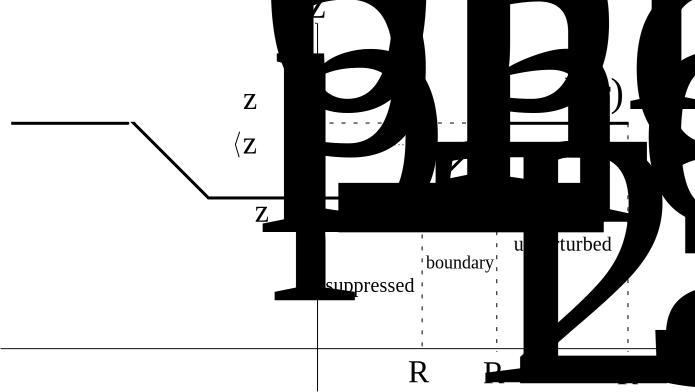
\includegraphics[width=0.7\textwidth]{./figures/Tat/MMs/linear_model}
  \caption[Simple model of the lateral decay of the membrane thickness 
  perturbation due to Tat]
  {Simple model of the lateral decay of the membrane thickness 
  perturbation due to Tat. The suppressed region is for $0 \leq r < \RTat$,
  the boundary region for $\RTat \leq r < R_2$, and the unperturbed
  region for $R_2 \leq < R_3$. $\zphos$ is the average $z$ position of
  phosphorus atoms measured from the bilayer center within the suppressed region.
  $\zphos$ was obtained directly from the MD simulation trajectories as described in 
  Sec.~\ref{sec:local_thinning}. $\zphos^0$ is the average $z$ position of 
  phosphorus atoms measured from the bilayer center in the unperturbed region.
  $\langle\zphos\rangle = \langle h(r)\rangle$ is half of the
  $\Dphos$ distance averaged over all lipids.}
  \label{fig:linear_model}
\end{figure}

Let us calculate $\langle h(r) \rangle$. In cylindrical coodinates, 
\begin{equation}
  \langle h(r) \rangle 
  = \frac{1}{\pi R_3^2} \int_0^{2\pi}d\phi \int_0^{R_3}\dr rh(r).
\end{equation}
The $\phi$ integration is trivial. The $r$ integration is
\begin{align}
  & \int_0^{R_3}\dr rh(r) \nonumber\\
  &= \int_0^{\RTat}\dr \zphos r + \int_{\RTat}^{R_2}\dr (mr+b)r + \int_{R_2}^{R_3}\dr \zphos^0r \nonumber\\
  &= \frac{1}{2}\left[\zphos \RTat^2+\zphos^0(R_3^2-R_2^2)\right] + 
     \frac{1}{3}m\left(R_2^3-\RTat^3\right) + 
     \frac{1}{2}b\left(R_2^2-\RTat^2\right) \nonumber\\        
  &= \frac{1}{2}\left[\zphos \RTat^2+\zphos^0(R_3^2-R_2^2)\right] +
     \frac{1}{3}\left(\zphos^0-\zphos\right)\left(R_2^2+\RTat R_2+\RTat^2\right) \nonumber\\
  &  + \frac{1}{2}\left(\zphos R_2-\zphos^0 \RTat\right)\left(\RTat+R_2\right). 
  \label{eq:r_integ}
\end{align}
Using Eq.~(\ref{eq:r_integ}), we get 
\begin{equation}
  \langle h(r) \rangle 
  = \frac{\left(\zphos-\zphos^0\right)\left(\RTat^2+\RTat R_2+R_2^2\right)+3\zphos^0R_3^2}{3R_3^2}.
  \label{eq:quadR2}
\end{equation}
Eq.~\ref{eq:quadR2} is a quadratic equation in terms of $R_2$. 
Solving for $R_2$ gives
\begin{equation}
  R_2 = \frac{-\RTat+\sqrt{\RTat^2+4C}}{2} 
\end{equation}
with
\begin{equation}
  C = \frac{3R_3^2\left(\zphos^0-\langle h(r)\rangle\right)}{\zphos^0-\zphos} - \RTat^2.
\end{equation}

%%%%%%%%%%%%%%%%%%%%%%%%%%%%%%%%%%%%%%%%%%%%%%%%%%%%%%%%%%%%%%%%%%%%%%%%%%%%%%%
\section{Results}
\subsection{Bending and Bulk Modulus}\label{sec:Kc_results}
Fig.~\ref{fig:figure1} shows the X-ray scattering intensity pattern from 
DOPC/DOPE (1:1) with Tat mole fraction $\xTat=0.034$. The diffuse lobes are 
due to equilibrium fluctuations that occur in these fully hydrated, oriented 
lipid/peptide samples. The intensity $I(\mathbf{q})$ in the diffuse 
patterns provide the absolute values of the form factors $F(q_z)$, which are 
the Fourier transforms of the electron density 
profile, through the relation $I(\mathbf{q})=S(\mathbf{q})|F(q_z)|^2/q_z$, 
where $\mathbf{q}=(q_r,q_z)$, $S(q)$ is 
the structure
interference factor, and $q_z^{-1}$ is the usual LAXS approximation to the 
Lorentz factor \cite{Kucerka05_BPJ,Kucerka06,Kucerka05_JMB}.
The first step in the analysis takes advantage of the $q_r$ dependence of the 
scattering to obtain the
bending modulus $K_c$ with results shown in Fig.~\ref{fig:figure2}. 
As positively charged Tat concentration was increased, 
the lamellar repeat spacing $D$ generally increased in neutral lipid 
bilayers and decreased in negatively charged bilayers, consistent with changes in 
electrostatic repulsive interactions. 
With few exceptions, the water space between bilayers exceeded 20 \AA.

\begin{figure}[htbp]
  \centering
  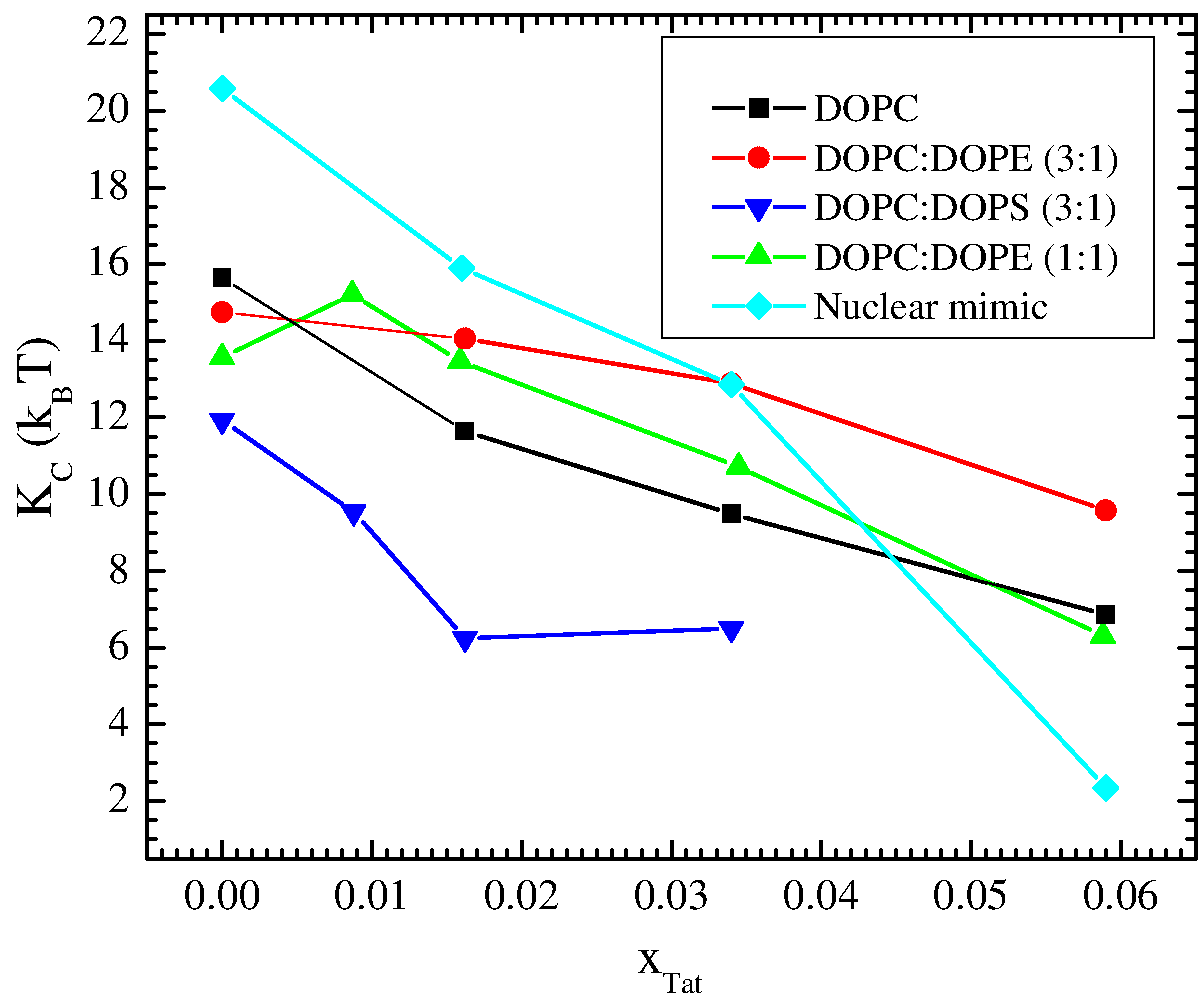
\includegraphics[width=0.8\textwidth]{figures/Tat/NFIT_results/Kc}
  \caption[Bilayer bending modulus, $K_c$, vs. Tat mole fraction $\xTat$]
  {Bilayer bending modulus, $K_c$, vs. Tat mole fraction $\xTat$. 
  $D$-spacings for DOPC:Tat mixtures varied from 64 to 68 \AA, 
  for DOPC:DOPE:Tat mixtures from 64 to 69 \AA, 
  for DOPC:DOPS:Tat (3:1) mixtures from 57 \AA\ to $>$ 100 \AA\ (pure DOPS was unbound), 
  and for nuclear mimic:Tat mixtures from unbound (nuclear mimic) to 64 \AA. 
  Estimated uncertainty in all values is  $\sim\pm$ 2.}
  \label{fig:figure2}
\end{figure}

\subsection{Form Factors}\label{sec:form_factors_results}
From the $K_c$ and $B$ values obtained via the diffuse scattering analysis,
the structure factor $S(\mathbf{q})$ is calculated, which leads to
the absolute form factors $|F(q_z)|=I(\mathbf{q})/S(\mathbf{q})$. 
To estimate uncertainties on $|F(q_z)|$, we analyzed multiple diffuse 
scattering data obtained by sampling different lateral positions for each sample,
which gave multiple form factors for a given sample.
These form factors were averaged to give the average form factors
and standard deviations for that sample (Fig.~\ref{fig:form_factor_uncertainty}).
Due to a small number of data sets for each sample, these standard
deviations were noisy, so they were smoothed over adjacent 20 points.
Average absolute form factors for five different membrane mimics are shown in 
Fig.~\ref{fig:form_factor1}--\ref{fig:form_factor4}. 
Vertical dashed lines indicate the ``zero'' position between the lobes of diffuse data 
where $F(q_z)$ change sign. In almost all samples, the zero positions shift to larger
$q_z$ as Tat mole fraction increased, indicating a thinning of the membranes. The thinning effect will be
quantified by fitting experimental form factors to models as will be discussed in
Sec.~\ref{sec:SDP_results}.

\begin{figure}[htbp]
  \centering
  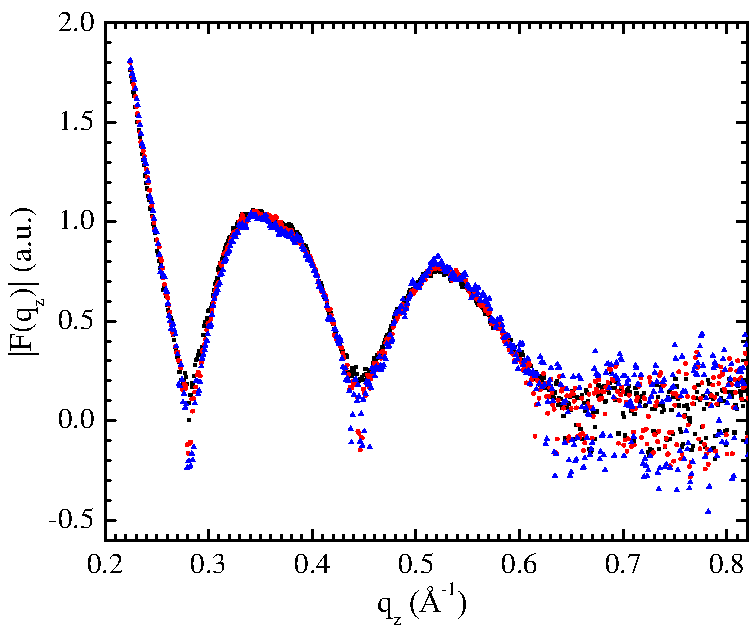
\includegraphics[width=0.45\textwidth]{figures/Tat/NFIT_results/three_form_factors}
  \\
  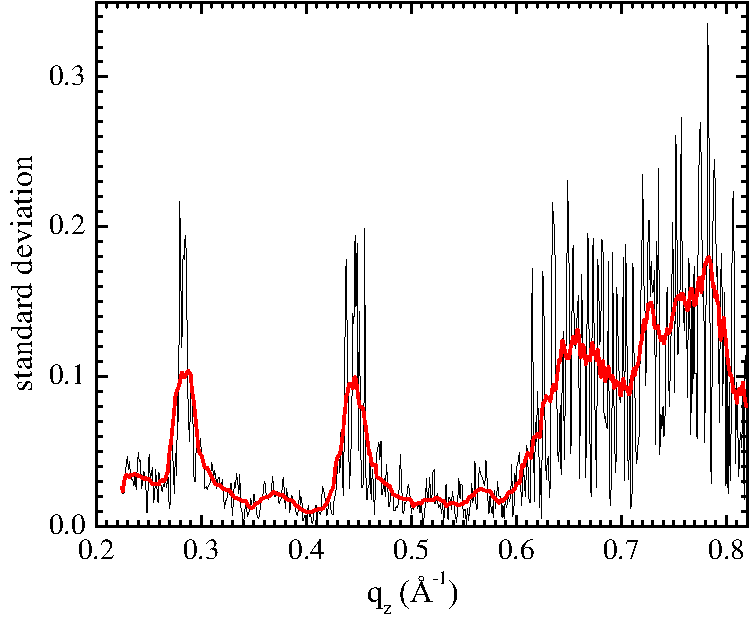
\includegraphics[width=0.45\textwidth]{figures/Tat/NFIT_results/standard_deviation}
  \caption[Three form factors obtained for three different lateral positions
  on a DOPC/Tat mixture with Tat mole fraction $\xTat$ = 0.016 (top)]
  {Three form factors obtained for three different lateral positions
  on a DOPC/Tat mixture with Tat mole fraction $\xTat$ = 0.016 (top).
  Standard deviations calculated by averaging these form factors are shown
  by black solid line (bottom). Because of the small number of data sets, the 
  uncertainties are noisy, so for a model fitting purpose, they were smoothed
  over adjacent 20 points (red solid line).}
  \label{fig:form_factor_uncertainty}
\end{figure}

\begin{figure}[htbp]
  \centering
  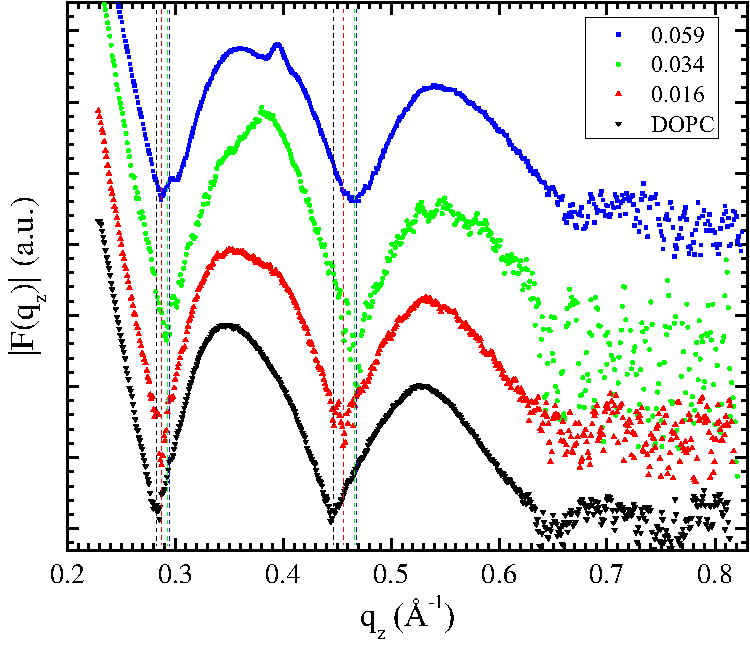
\includegraphics[width=\textwidth]{figures/Tat/NFIT_results/DOPC_form_factors}
  \caption[Form factors of DOPC with Tat mixtures (arbitrarily scaled and vertically 
  displaced) with increasing Tat mole fractions $\xTat$ indicated on figure 
  legend]
  {Form factors of DOPC with Tat mixtures (arbitrarily scaled and vertically 
  displaced) with increasing Tat mole fractions $\xTat$ indicated on figure 
  legend. 
  Dashed vertical lines roughly indicate the $q_z$ values where the form factors are equal 
  to zero between the lobes of diffuse data.
  Error bars are omitted for clarity.}
  \label{fig:form_factor1}
\end{figure}

\begin{figure}[htbp]
  \centering
  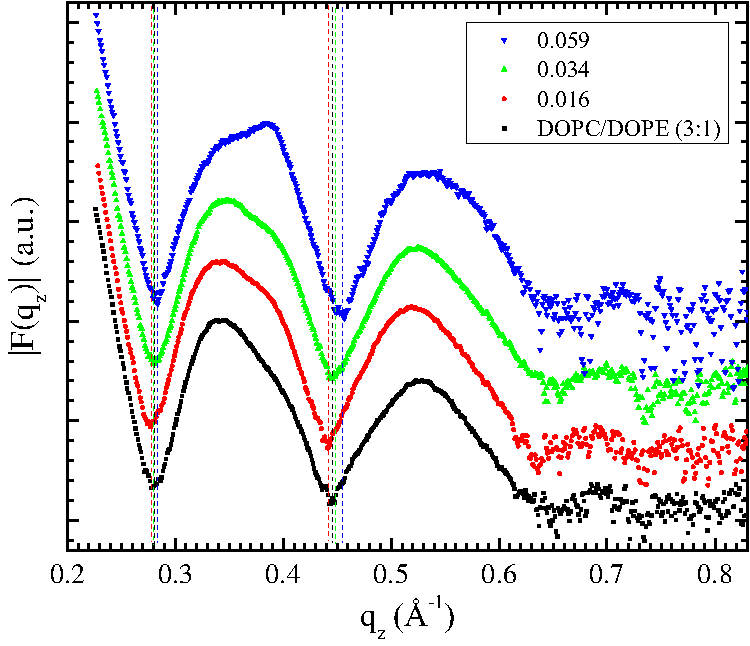
\includegraphics[width=\textwidth]{figures/Tat/NFIT_results/DOPCDOPE3to1_form_factors}
  \caption[Form factors of DOPC:DOPE (3:1) with Tat mixtures]
  {Form factors of DOPC:DOPE (3:1) with Tat mixtures.
  The rest of the caption is the same as in Fig.~\ref{fig:form_factor1}.}
  \label{fig:form_factor2}
\end{figure}

\begin{figure}[htbp]
  \centering
  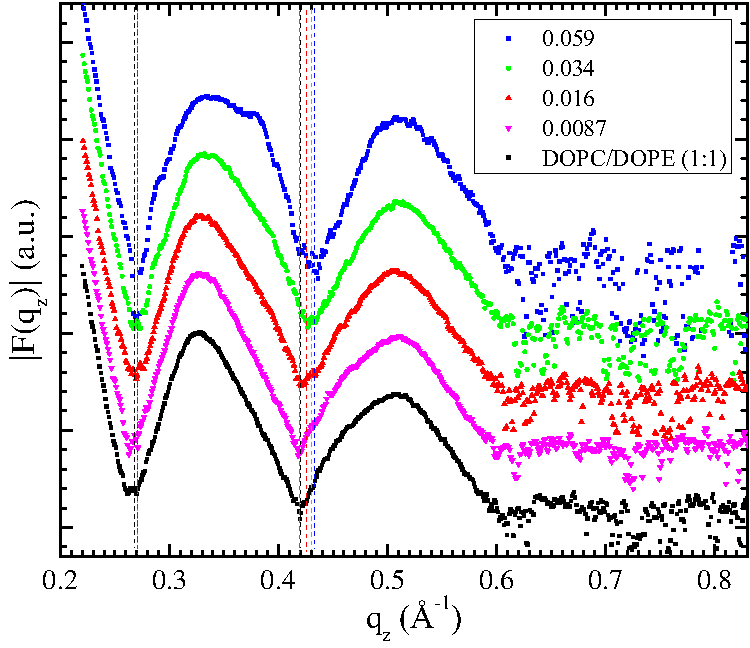
\includegraphics[width=\textwidth]{figures/Tat/NFIT_results/DOPCDOPE1to1_form_factors}
  \caption[Form factors of DOPC:DOPE (1:1) with Tat mixtures]
  {Form factors of DOPC:DOPE (1:1) with Tat mixtures.
  The rest of the caption is the same as in Fig.~\ref{fig:form_factor1}.}
  \label{fig:form_factor3}
\end{figure}

\begin{figure}[htbp]
  \centering
  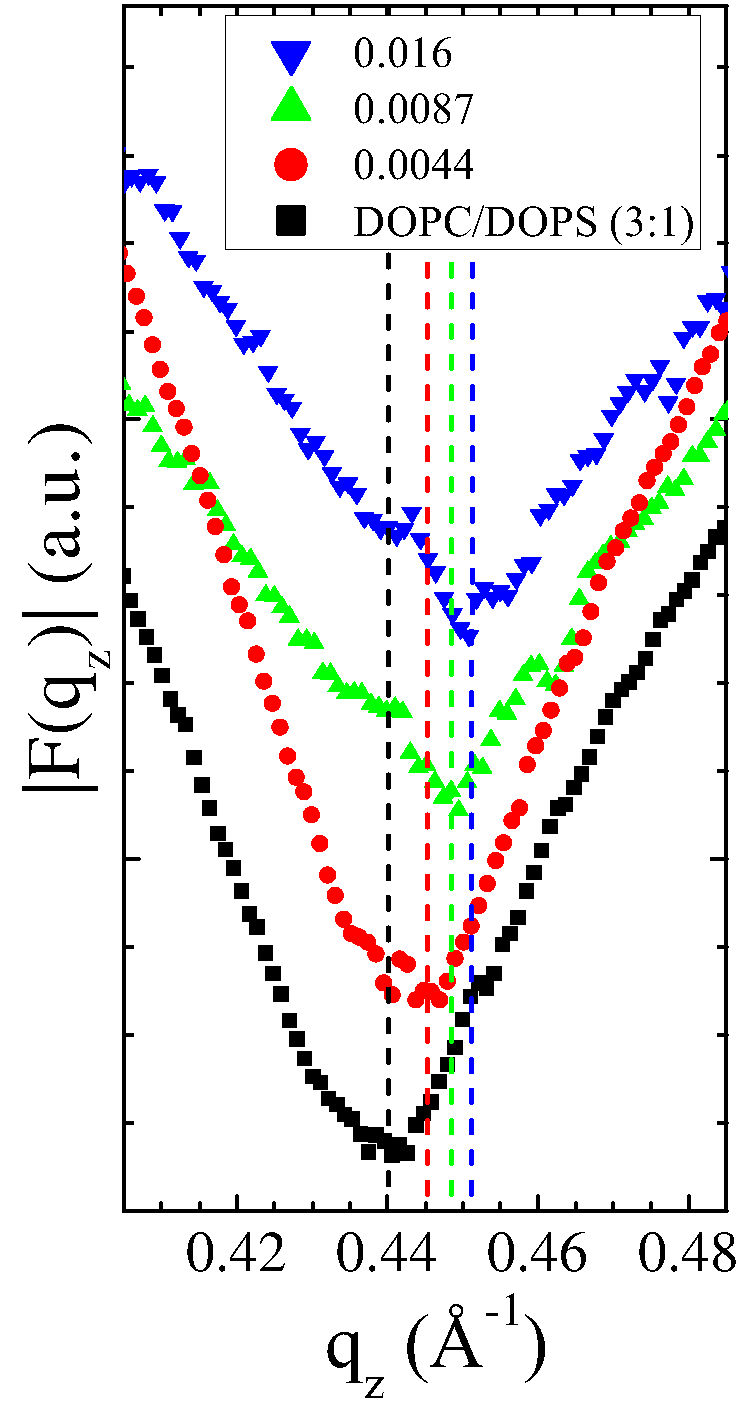
\includegraphics[width=0.3\textwidth]{figures/Tat/NFIT_results/DOPCDOPS3to1_form_factors}
  \qquad  
  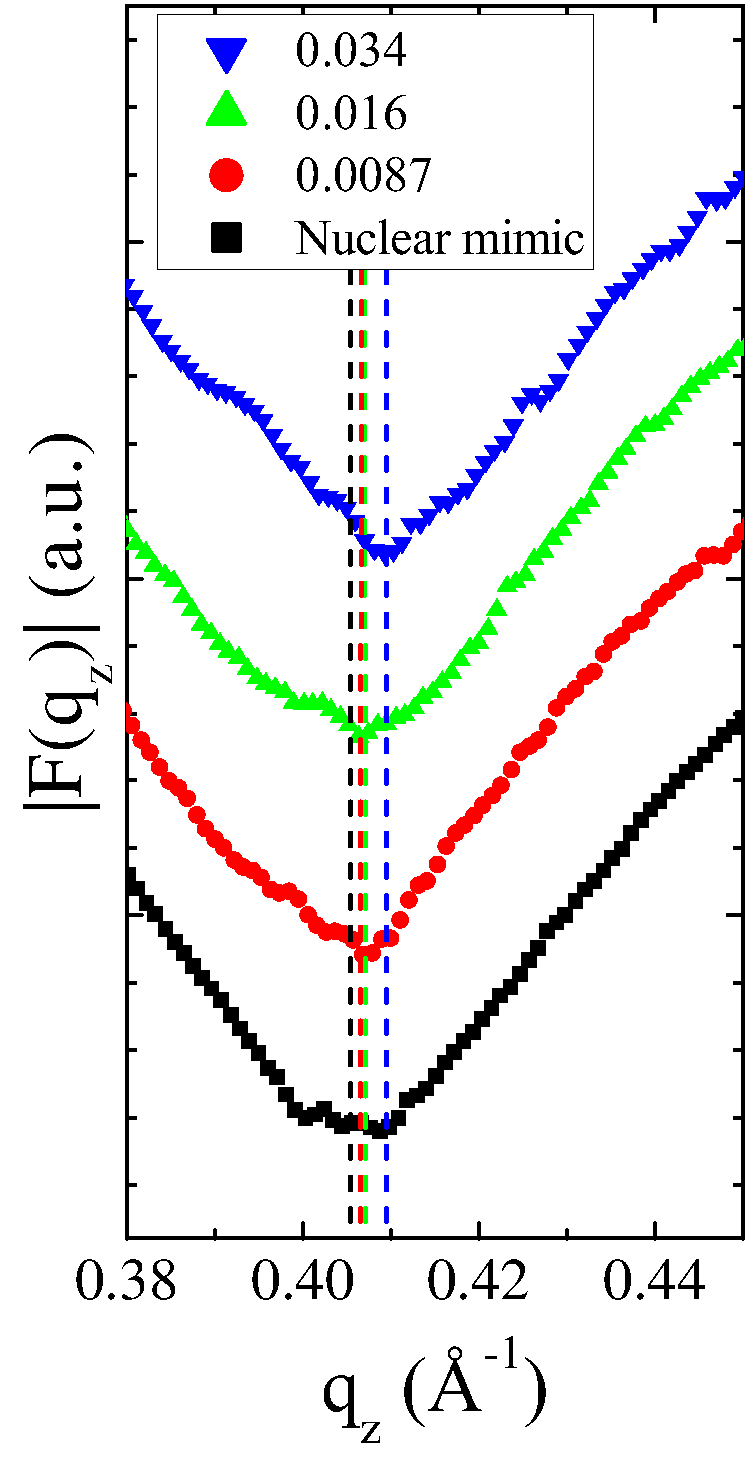
\includegraphics[width=0.3\textwidth]{figures/Tat/NFIT_results/nuclear_form_factors}
  \caption[Form factors of DOPC:DOPS (3:1) (left) and nuclear membrane mimic 
  (right) with Tat mixtures]
  {Form factors of DOPC:DOPS (3:1) (left) and nuclear membrane mimic 
  (right) with Tat mixtures.
  Portions of the form factors $|F(q_z)|$ that were not significantly distorted 
  by mosaic spread scattering are shown.
  The most of the caption is the same as in Fig.~\ref{fig:form_factor1}.}
  \label{fig:form_factor4}
\end{figure}

%%%%%%%%%%%%%%%%%%%%%%%%%%%%%%%%%%%%%%%%%%%%%%%%%%%%%%%%%%%%%%%%%%%%%%%%%%%%%%%
\newpage
\subsection{Volume}\label{sec:volume_results}
Experimental and simulated volumes are given in Table~\ref{tab:volumes}. The simulated volume was
obtained using the volume app (REF. for Petrache 97) in the SIMtoEXP program \cite{Kucerka10}. The experimental Tat volume was
calculated from the measured density assuming that the lipid volume was the same as with no
Tat. In general, there may be an interaction volume between the peptide and the lipid membrane
as previously reported for bacteriorhodopsin \cite{Tristram-Nagle86}. As lipid was present in excess to Tat, the
partial molecular volume of the lipid is the same as with no Tat, so this way of
calculating includes all the interaction volume in $\VTat$. Comparison of $\VTat$ in water with the
result for 5:1 Lipid:Tat suggests that the interaction volume may be negative, consistent with a
net attractive interaction with lipid. Understandably, values of $\VTat$ were unreliable for small
mole ratios of Tat:Lipid. Therefore we used simple additivity for those mimics not shown in
Table~\ref{tab:volumes} for the volumes used in the electron density profile modeling. 
All volumes obtained from the Gromacs MD
simulations were somewhat smaller than the measured volumes, but it supports the Tat volume
being closer to 1877 \AA$^3$ than the outlying values obtained experimentally at small Tat
concentrations. The measured volume is in good agreement with the 
value calculated from a peptide calculator website \cite{peptide_calc}, which
gave 1888 \AA$^3$. 

%------------------------------------------------------------------------------
%\begin{table}[htbp]
%  \centering
%  \begin{tabular}{c c}
%    $\rho_{sol}$ & 0.994180 $\mathrm{g/cm^3}$\\
%    $\rho_w$ & 0.993325 $\mathrm{g/cm^3}$\\
%    $m_w$ & 1212.6 mg \\
%    $m_T$ & 3.73 mg \\ 
%  \end{tabular}
%  \caption{Measured Quantities in }
%  \label{tab:values}
%\end{table}

\begin{table}[htbp]
  \centering
  Experiments\\
  \begin{tabular}{cccc}
    \hline
    Tat in: & $V_\textrm{lipid}$ (\AA$^3$) & $\xTat$ & $\VTat$ (\AA$^3$) \\
    \hline
    water & & & 1877 \\
    DOPC:DOPE (3:1) & 1288 & 0.167 & 1822 \\
    DOPC & 1314 & 0.0246 & 676 \\
    DOPC:DOPS (3:1) & 1298 & 0.0246 & 2613 \\
    \hline 
  \end{tabular}
  \quad
  \begin{tabular}{cccc}
    & & & \\
    \multicolumn{4}{c}{Simulations} \\ 
    \hline
    Tat in: & $V_\textrm{lipid}$ (\AA$^3$) & Lipid:Tat & $\VTat$ (\AA$^3$) \\
    \hline
    DOPC & 1283 & 128:2 & 1694 \\
    DOPC & 1294 & 128.4 & 1699 \\
    \hline
  \end{tabular}
  \caption[Volume results at 37 \textcelsius]
  {Volume results at 37 \textcelsius.}
  \label{tab:volumes}
\end{table}

%%%%%%%%%%%%%%%%%%%%%%%%%%%%%%%%%%%%%%%%%%%%%%%%%%%%%%%%%%%%%%%%%%%%%%%%%%%%%%%
\newpage
\subsection{Electron Density Profile Modeling}\label{sec:SDP_results}
We fit our measured X-ray form factors to the Tat-in-headgroup (THG) model described in 
Sec.~\ref{sec:SDP_method}. In all fits,
the positions of component groups were free parameters, but we 
assumed that the lipid headgroup is somewhat rigid so that it cannot compress
or expand. This assumption led to fixing the distance
$\zPC-\zCG$ between the PC and CG components as well
as the distance $\zCG-\zHC$ between the CG component and the Gibbs dividing
surface for the hydrocarbon chains. 
We also constrained the width of Tat 
Gaussian $\sigmaTat$. We fitted with three different values of widths,
2.5, 3.0, and 3.5, to study the range of variation due to the Tat width. 
We eventually constrained the Tat width 
because it tended to become unphysically small
when it was set free. Without higher $q_z$ data points, a very narrow feature
in an electron density profile, which results in large form factors at high $q_z$,
are not penalized.  

Table~\ref{tab:DOPC_fit_results} shows the model parameters that produced
the best fits for DOPC with Tat.
At lower Tat concentrations ($\xTat$ = 0.016 and 0.034), 
a smaller $\chi^2$ value was obtained for smaller $\sigmaTat$,
consistent with its tendency to become unphysically small as noted 
in the previous paragraph. The widths of the headgroups $\sigmaPC$ and
$\sigmaCG$ decreased from those of pure DOPC when Tat was added.  
It is also seen from Table~\ref{tab:DOPC_fit_results} 
that the area per lipid $\AL$ increased as the Tat concentration was
increased from 0 to 0.034. An increase in $\AL$ implies thinning of a bilayer because
a lipid bilayer can be approximated as an incompressible fluid membrane. 
Another observed trend was that $\zTat$ increased as $\xTat$ was increased.
Figure~\ref{fig:DOPC_Tat_XFF1} shows the best fits and corresponding 
electron density profiles for DOPC with Tat.

\begin{table}[htbp]
  \centering
  \begin{tabular}{c|c|ccc|ccc|ccc}
    \hline
    $\xTat$ & 0 & 0.016 & 0.016 & 0.016 & 0.034 & 0.034 & 0.034 & 0.059 & 0.059 & 0.059 \\
    \hline
    $\chi^2$ & 2961 & \textcolor{red}{1554} & 1570 & 1581 & \textcolor{red}{1563} & 1587 & 1607 & 2342 & \textcolor{red}{2338} & 2363 \\ 
    $\zPC$ & 18.1 & 18.0 & 17.9 & 17.9 & 17.8 & 17.7 & 17.6 & 17.8 & 17.8 & 17.7 \\
    $\sigmaPC$ & 2.52 & 2.14 & 2.17 & 2.18 & 1.86 & 1.92 & 1.93 & 2.02 & 1.97 & 1.93 \\
    $\zCG$ & 15.0 & 14.9 & 14.8 & 14.8 & 14.7 & 14.6 & 14.5 & 14.7 & 14.7 & 14.6 \\
    $\sigmaCG$ & 3.00 & 2.62 & 2.64 & 2.66 & 2.22 & 2.30 & 2.31 & 2.58 & 2.27 & 2.14 \\
    $\zHC$ & 13.7 & 13.6 & 13.5 & 13.5 & 13.4 & 13.3 & 13.2 & 13.4 & 13.4 & 13.3 \\ 
    $\sigmaHC$ & 3.00 & 2.69 & 2.84 & 2.95 & 2.65 & 2.82 & 3.01 & 2.47 & 2.58 & 2.83 \\
    $\sigmaCHthree$ & 3.20 & 3.19 & 3.22 & 3.24 & 3.37 & 3.43 & 3.47 & 2.70 & 2.70 & 2.74 \\
    $\zTat$ & NA & 12.9 & 13.4 & 14.2 & 13.1 & 13.8 & 14.4 & 15.2 & 15.2 & 15.7 \\
    $\sigmaTat$ & NA & 2.5* & 3.0* & 3.5* & 2.5* & 3.0* & 3.5* & 2.5* & 3.0* & 3.5* \\ 
    $\AL$ & 71.5 & 72.4 & 72.5 & 72.7 & 73.6 & 74.0 & 74.4 & 73.6 & 73.5 & 73.9 \\
    \hline
  \end{tabular}
  \caption[Fitting results for DOPC membranes for the THG (Tat in headgroup) model]
  {Fitting results for DOPC membranes for the THG (Tat in headgroup) model. 
  The smallest $\chi^2$ values at each Tat mole fraction $\xTat$ are highlighted in red.  
  $\zPC-\zCG = 3.1$ \AA\
  and $\zCG-\zHC = 1.3$ \AA\ in all fits.
  Units of all symbols are \AA\ except for $\chi^2$ (unitless) and $\AL$ (\AA$^2$).  
  \\
  *Paramters were fixed.}
  \label{tab:DOPC_fit_results}
\end{table}

\begin{figure}[htbp]
  \centering
  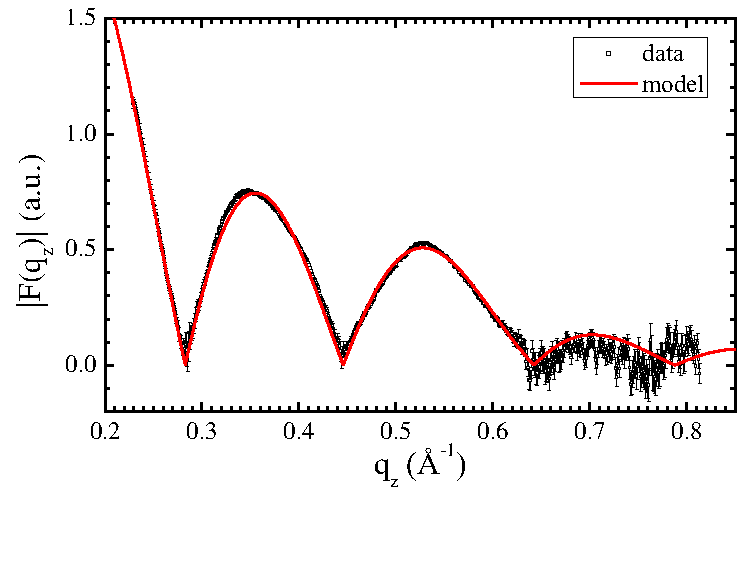
\includegraphics[trim=5 30 0 0,clip=true,width=0.47\textwidth]{figures/Tat/SDP_Results/XFF/DOPC_XFF1} 
  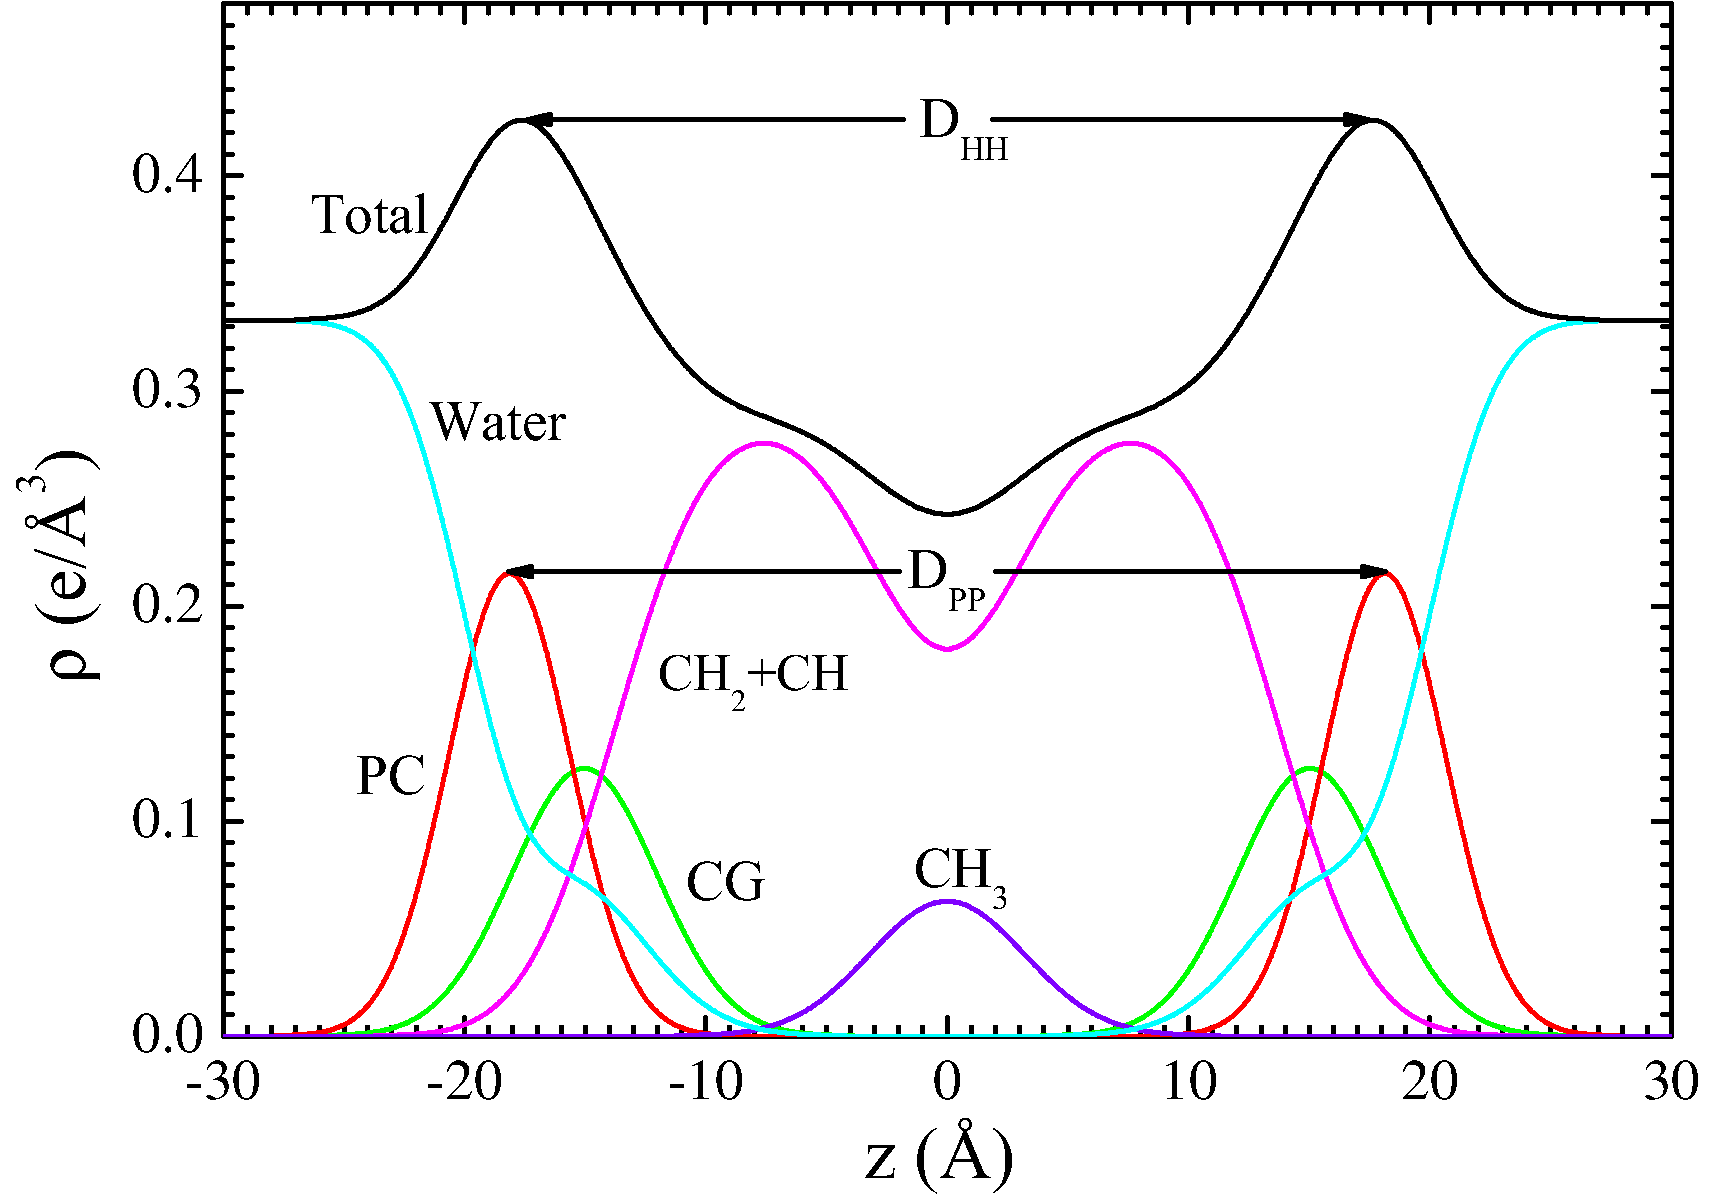
\includegraphics[trim=5 30 0 0,clip=true,width=0.47\textwidth]{figures/Tat/SDP_Results/EDP/DOPC_EDP1} 
  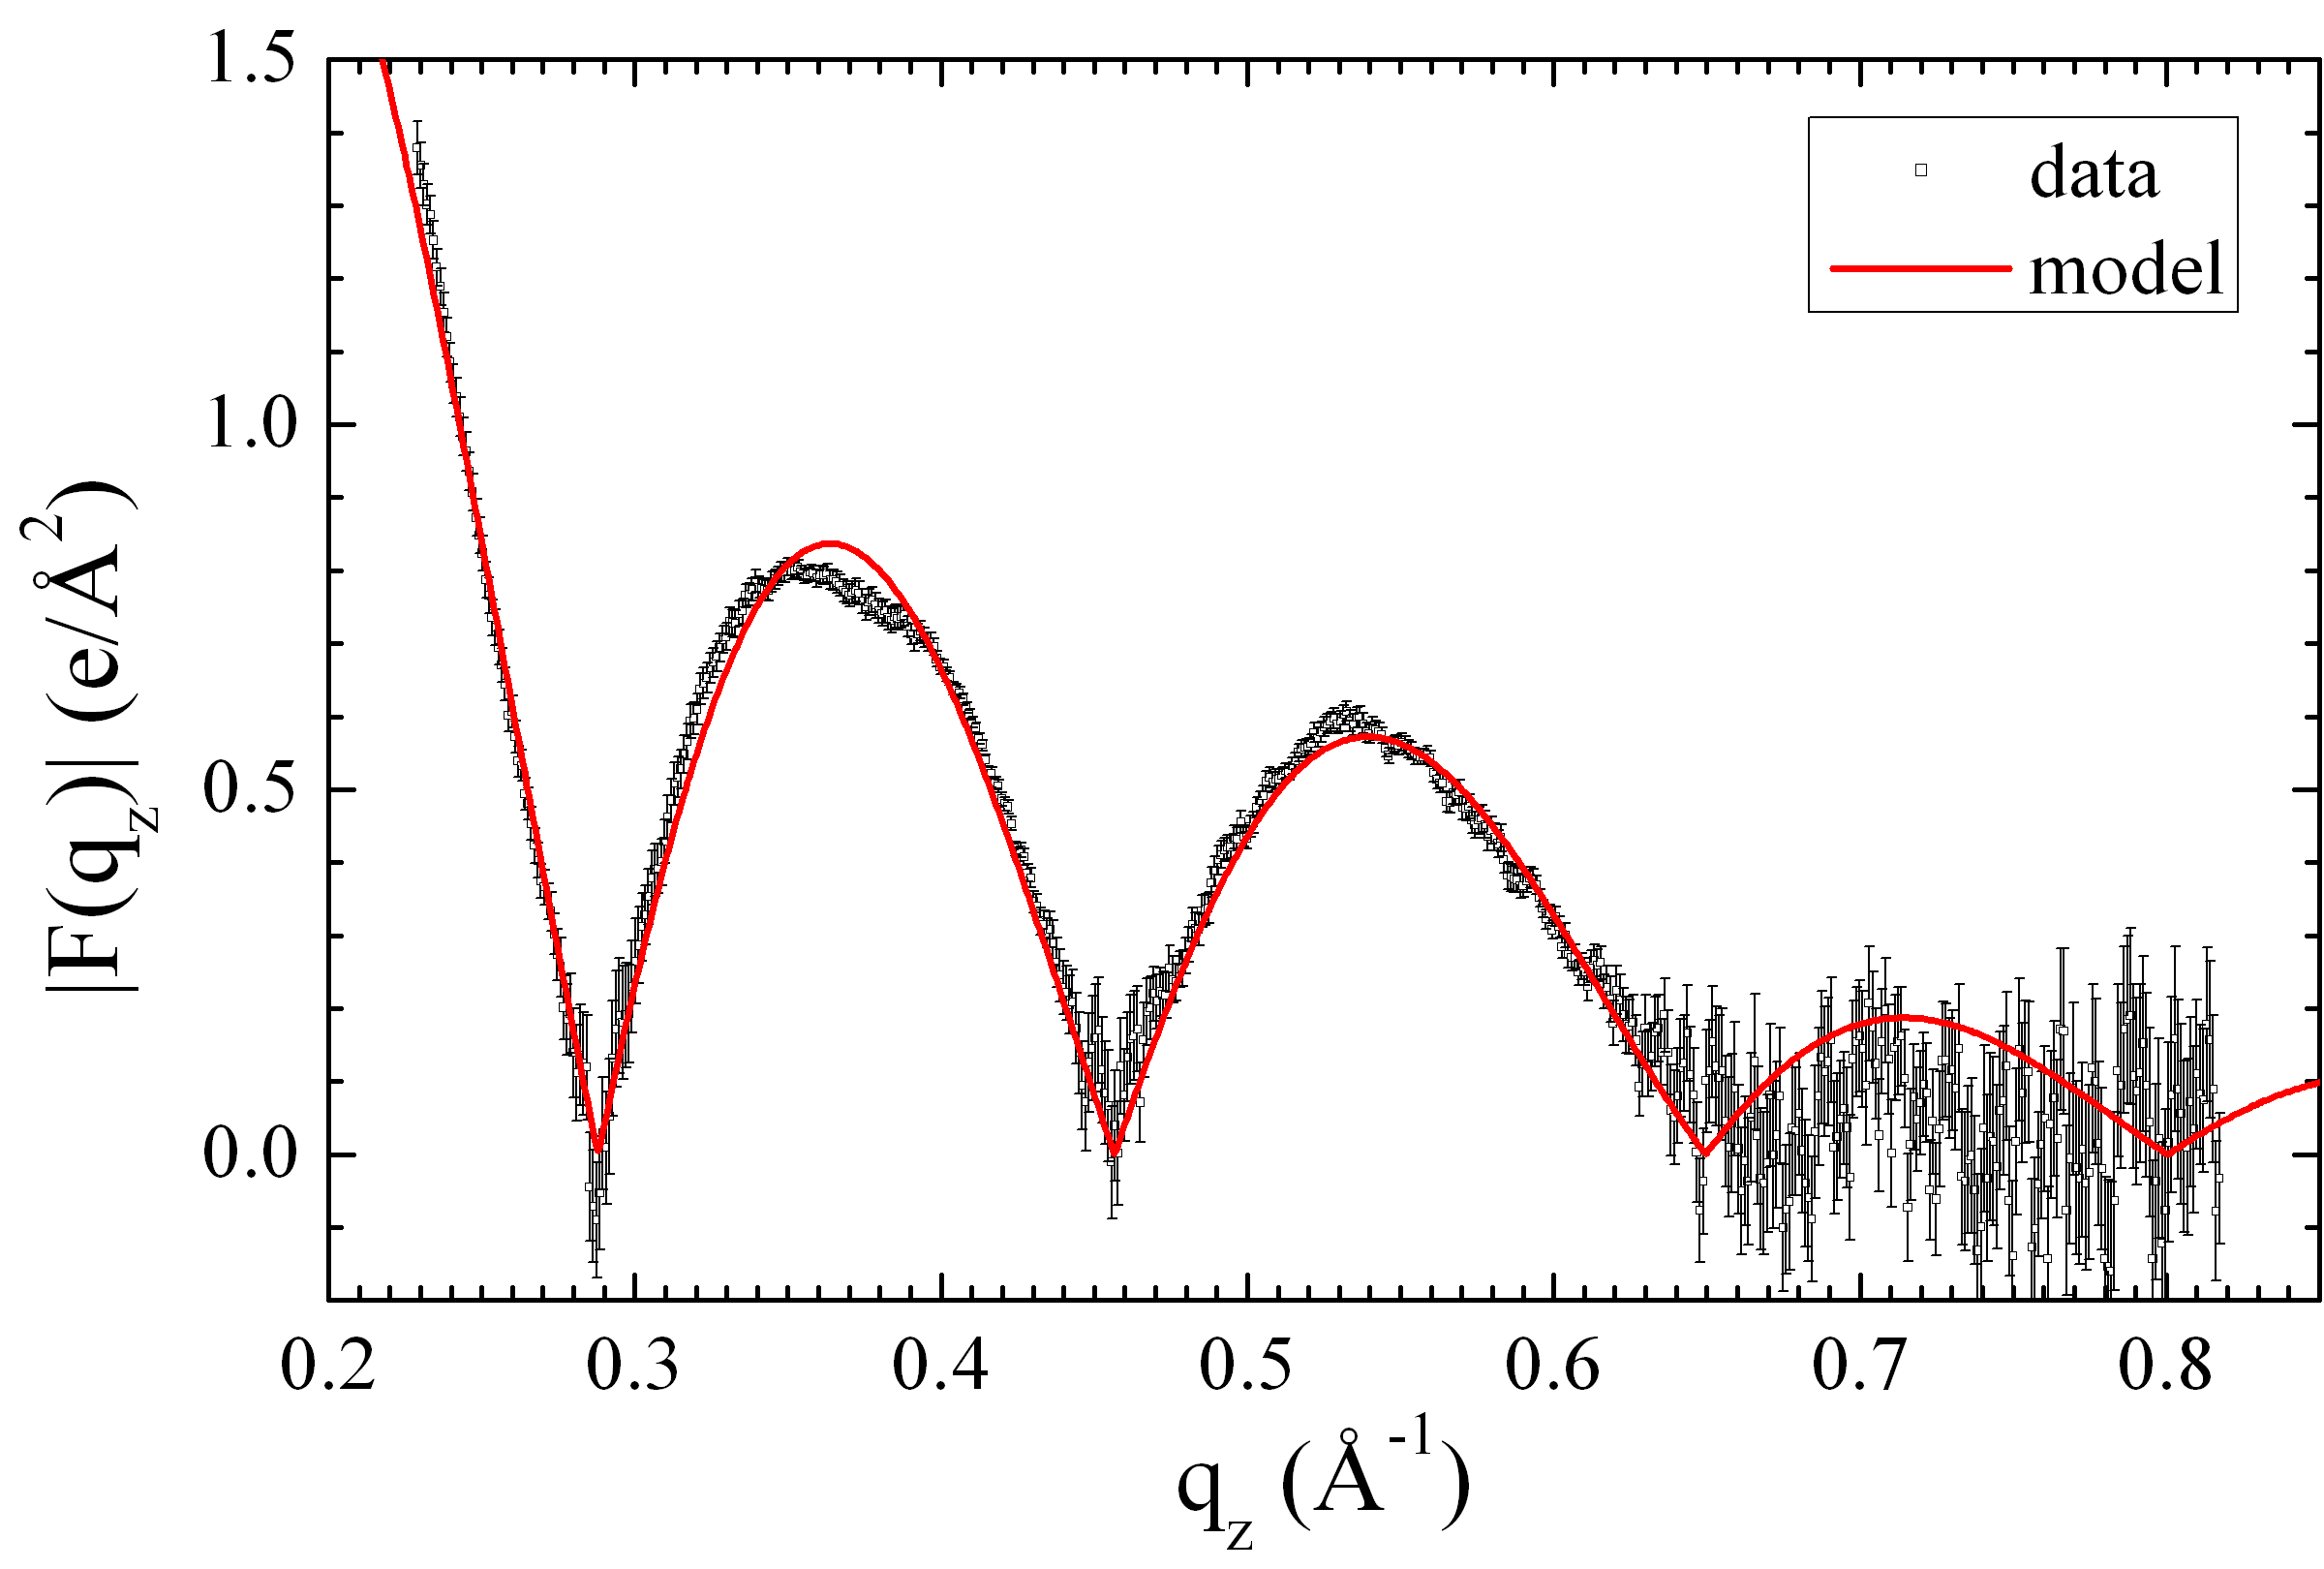
\includegraphics[trim=5 30 0 0,clip=true,width=0.47\textwidth]{figures/Tat/SDP_Results/XFF/DOPC_Tat_62to1_3p0_XFF1}
  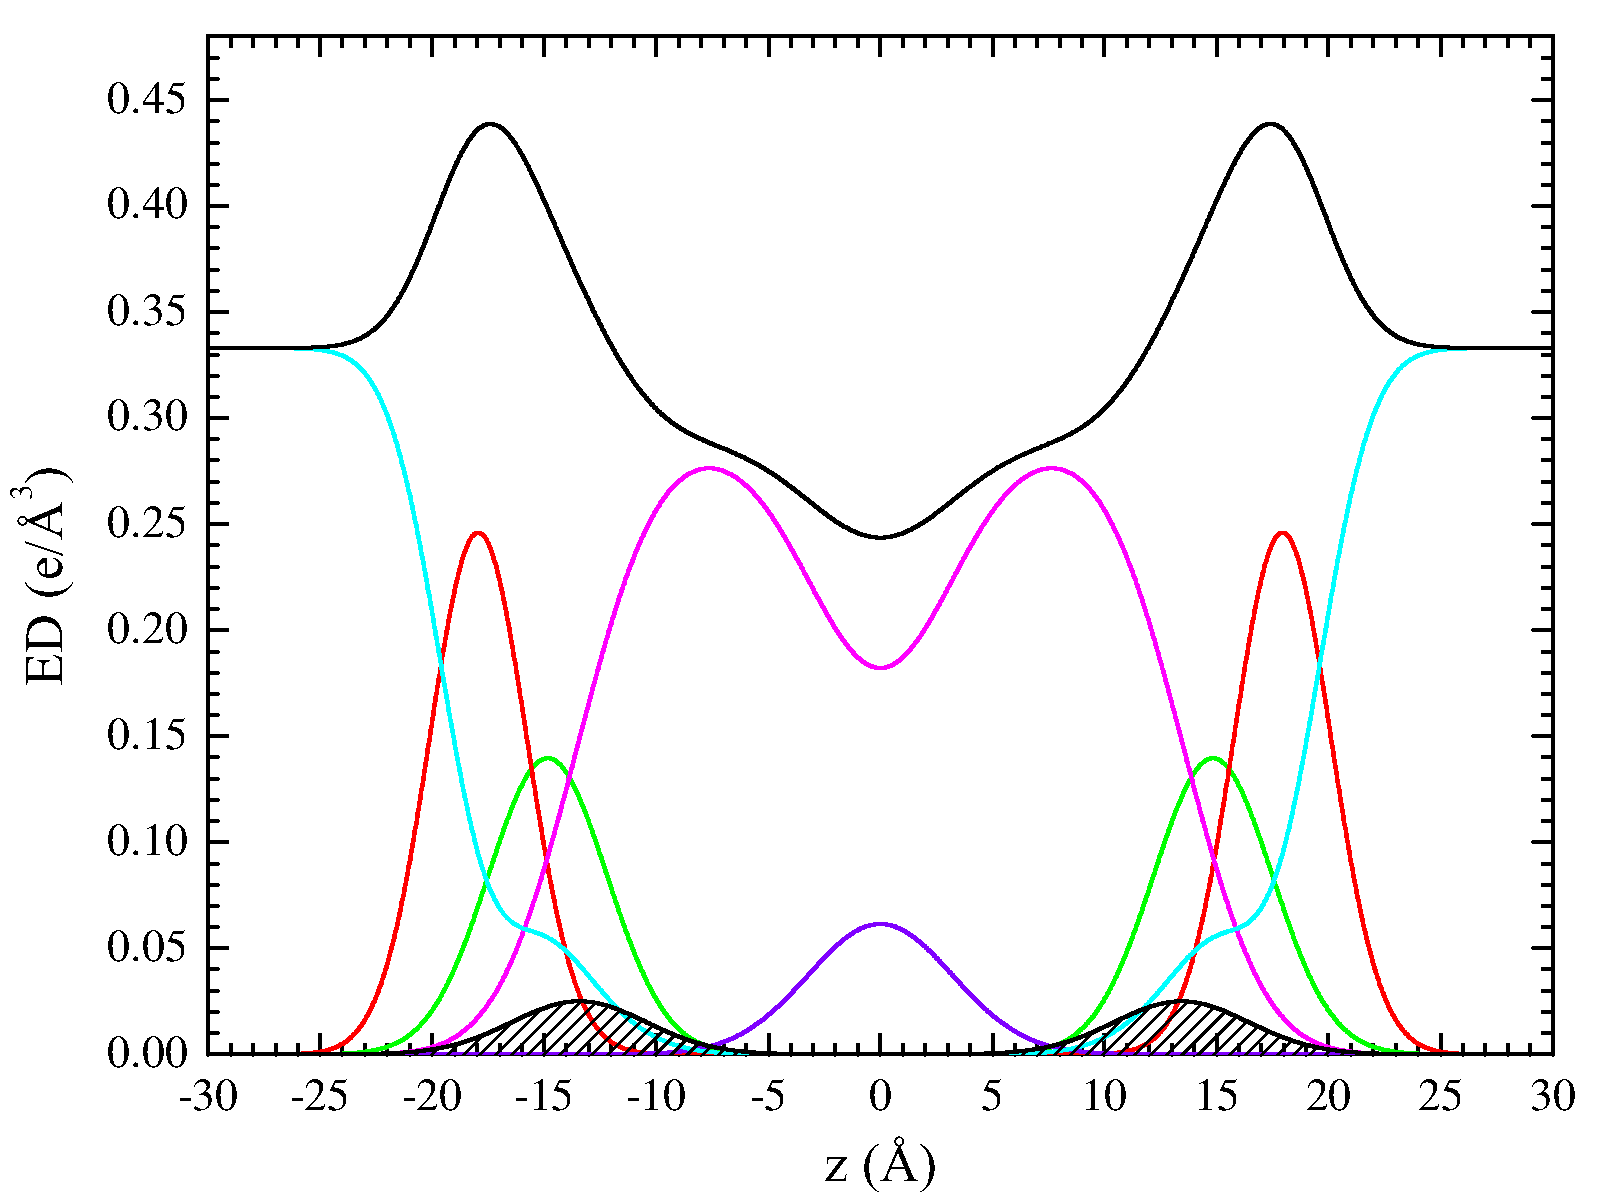
\includegraphics[trim=5 30 0 0,clip=true,width=0.47\textwidth]{figures/Tat/SDP_Results/EDP/DOPC_Tat_62to1_3p0_EDP1} 
  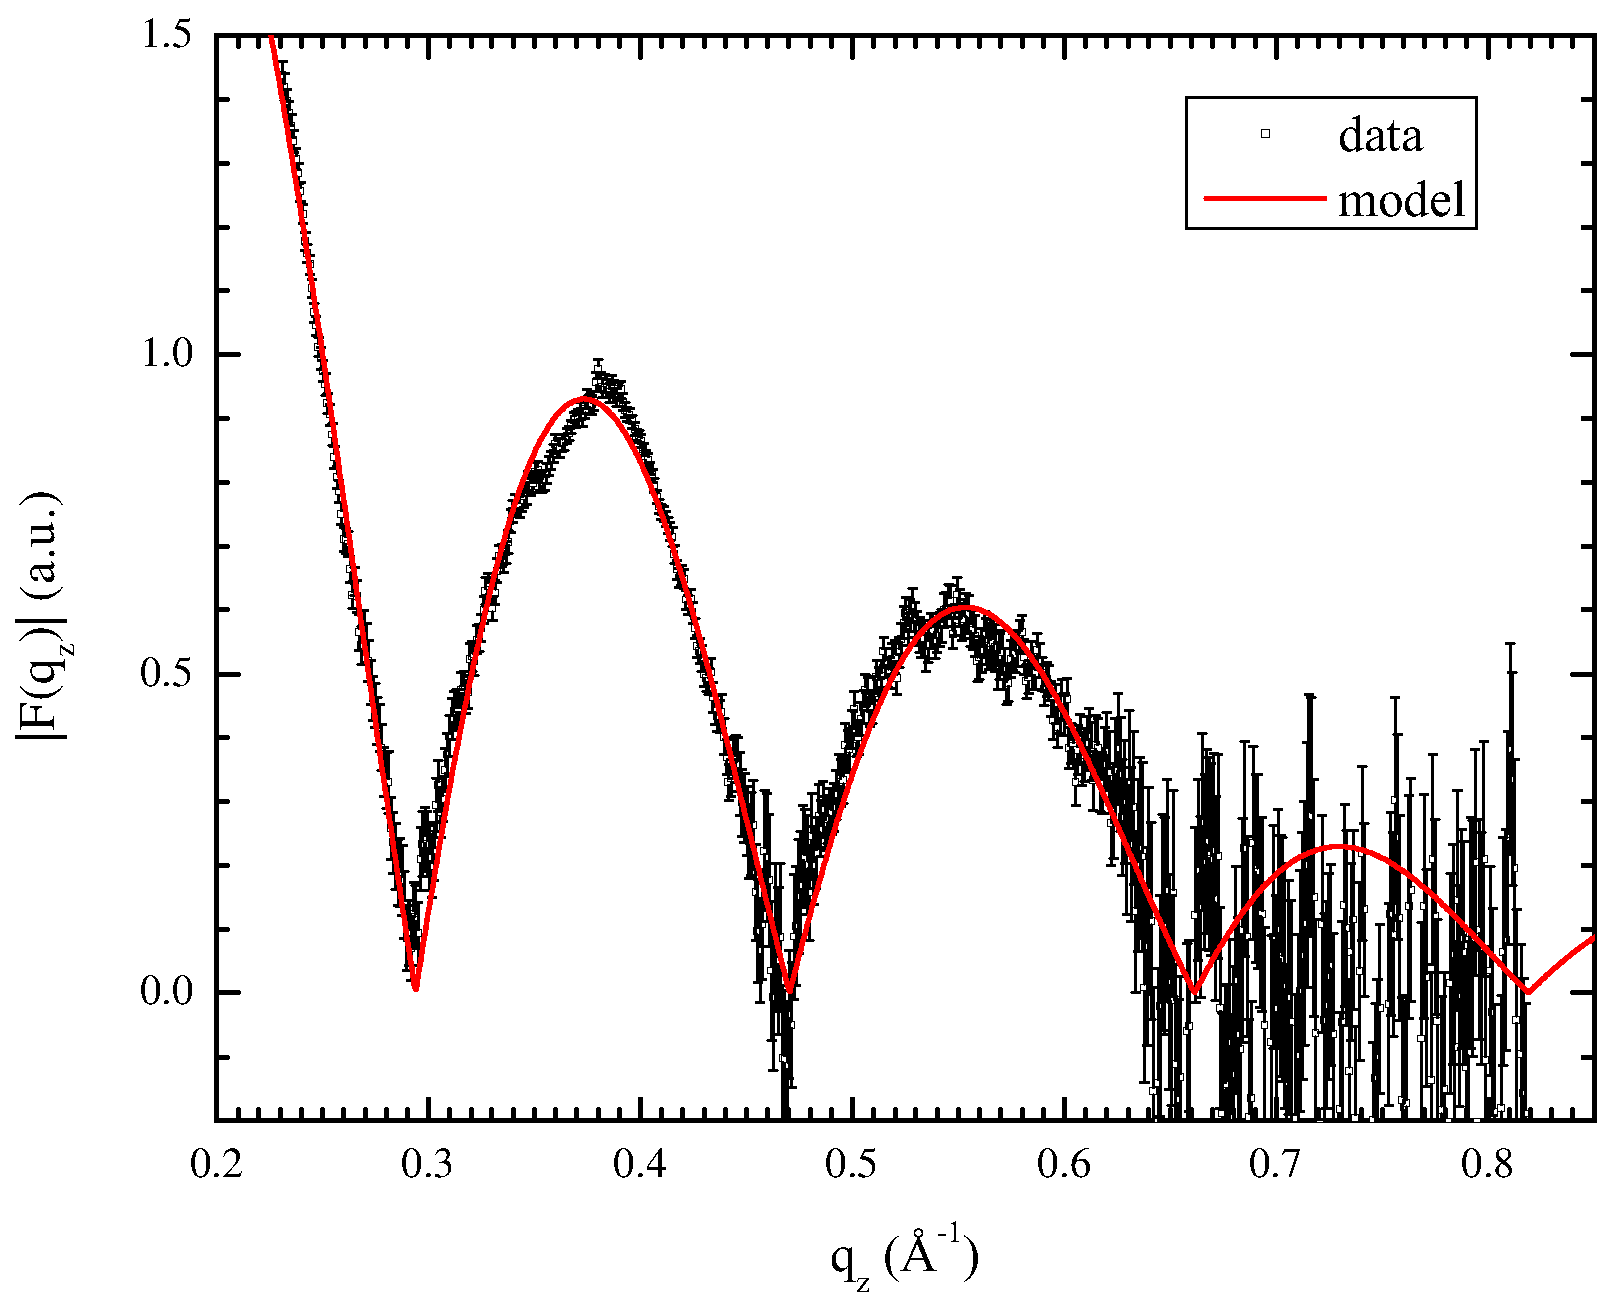
\includegraphics[trim=5 30 0 0,clip=true,width=0.47\textwidth]{figures/Tat/SDP_Results/XFF/DOPC_Tat_28to1_3p0_XFF1}
  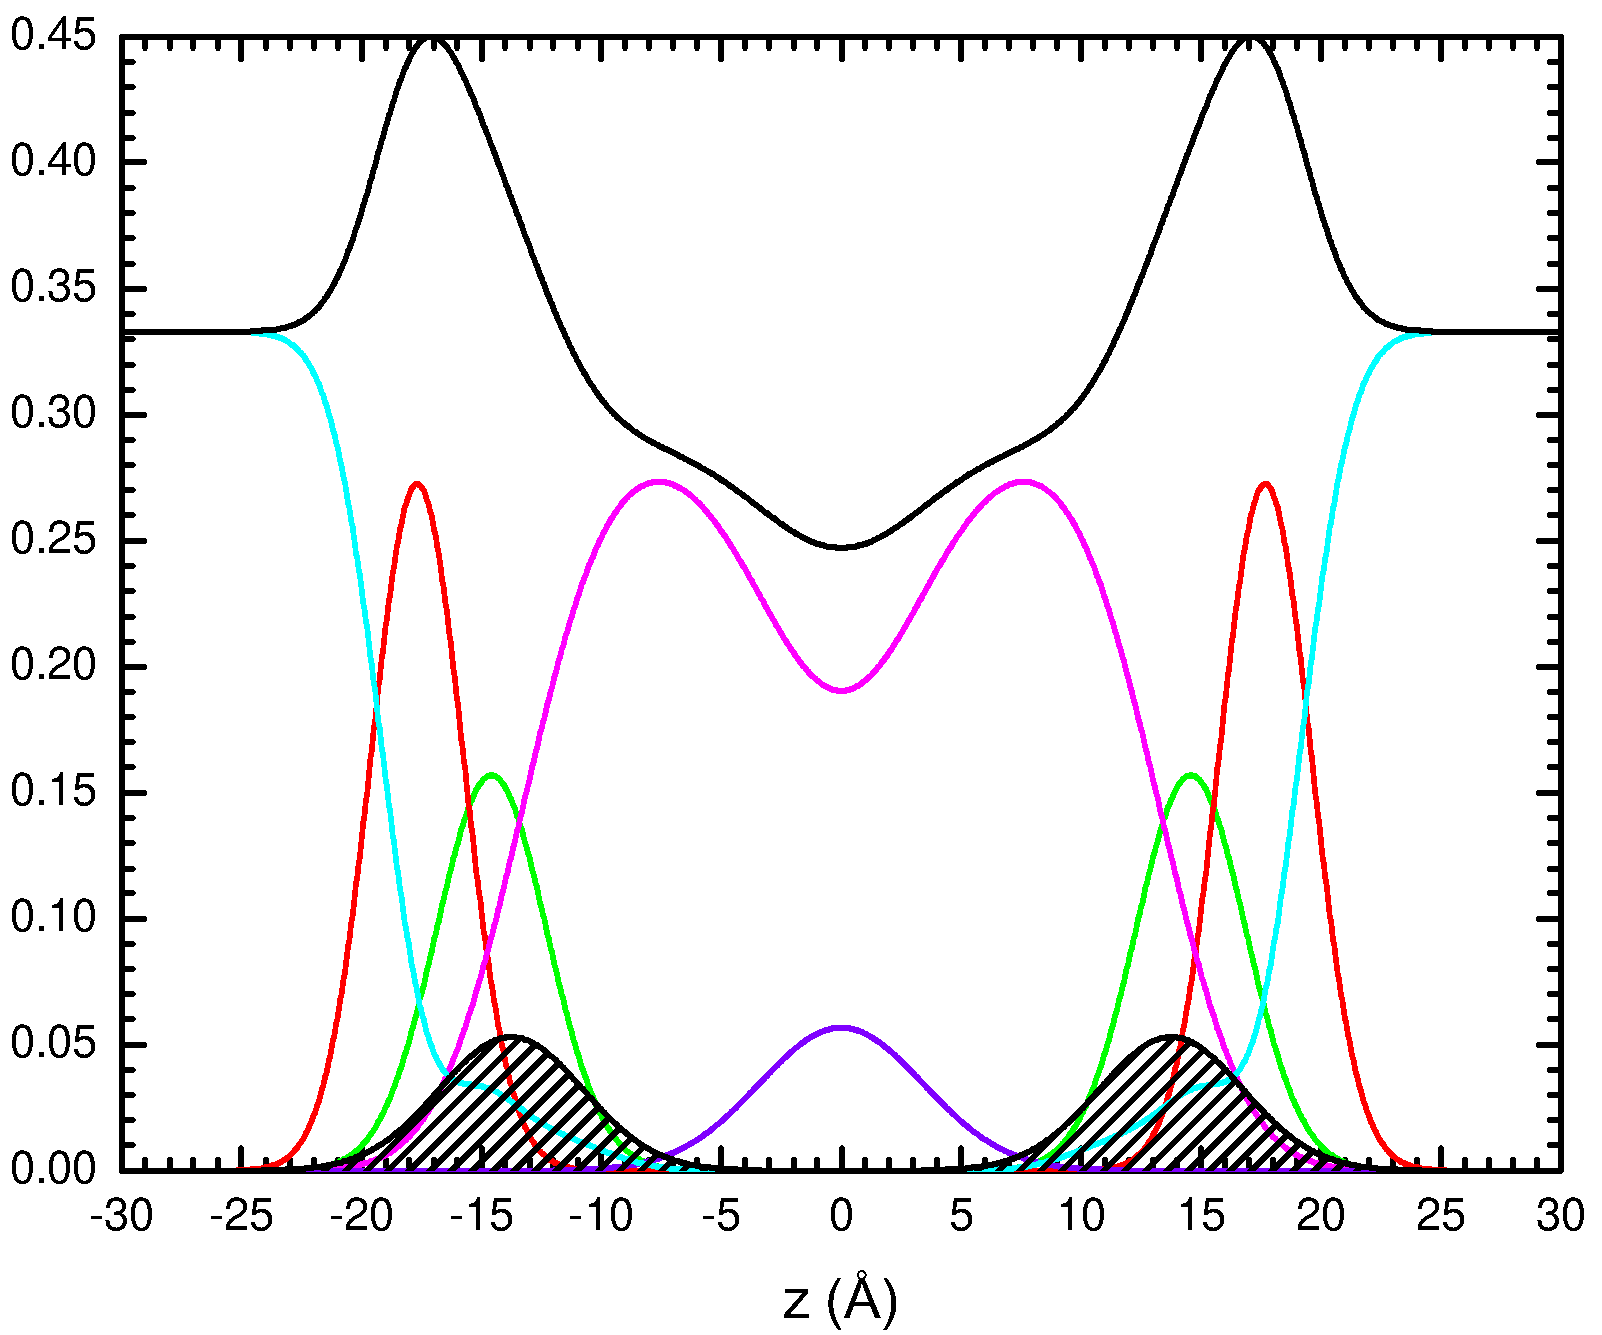
\includegraphics[trim=5 30 0 0,clip=true,width=0.47\textwidth]{figures/Tat/SDP_Results/EDP/DOPC_Tat_28to1_3p0_EDP1}
  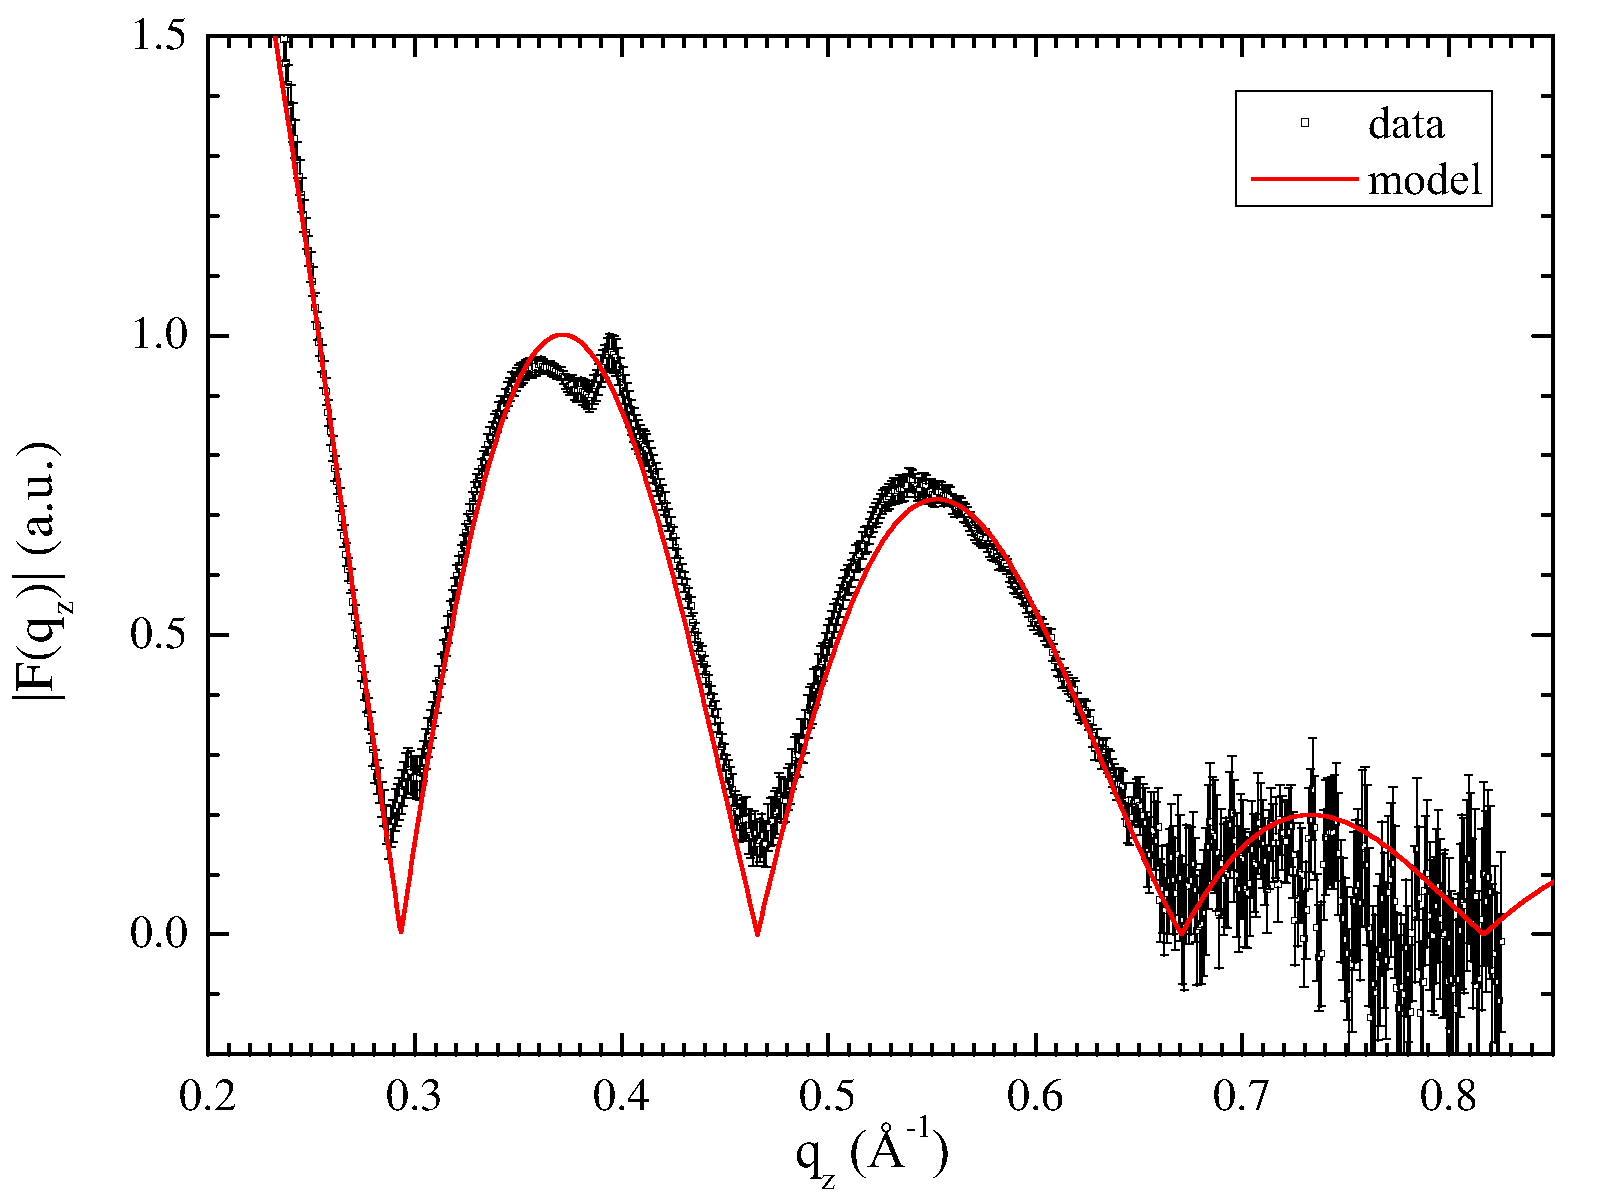
\includegraphics[trim=5 30 0 0,clip=true,width=0.47\textwidth]{figures/Tat/SDP_Results/XFF/DOPC_Tat_16to1_3p0_XFF1}
  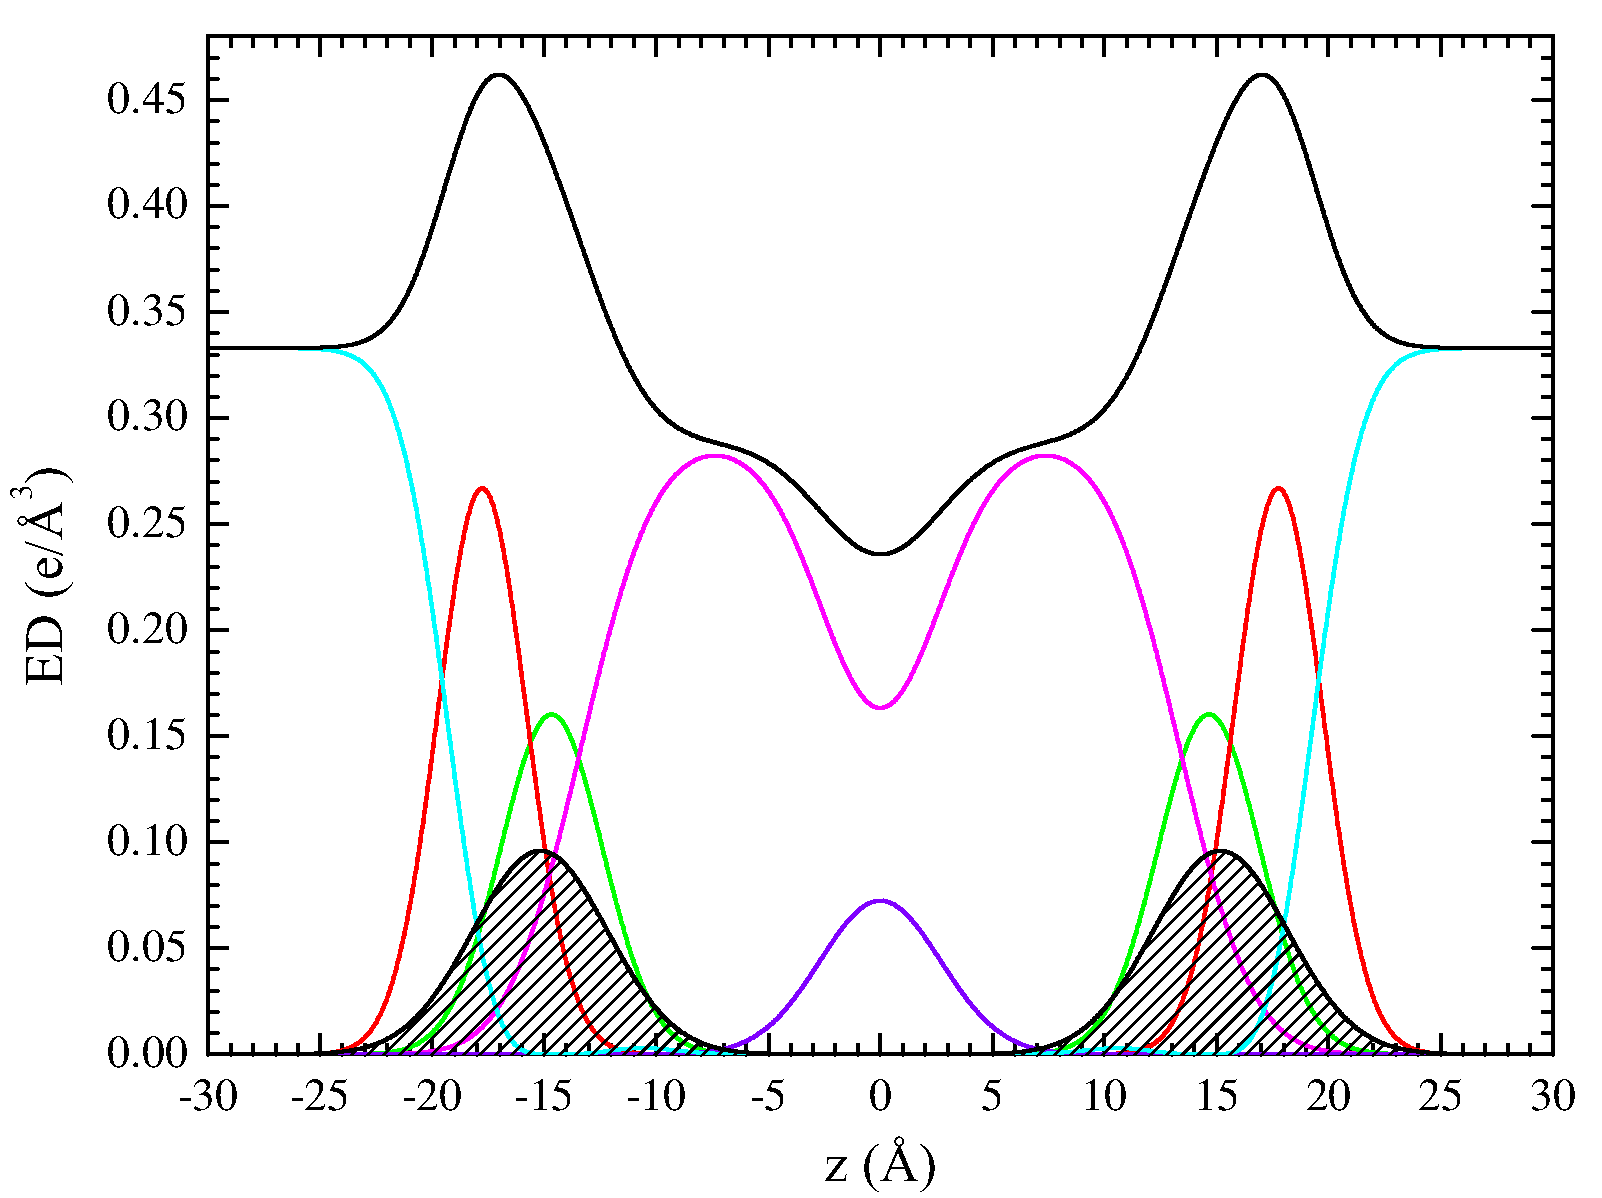
\includegraphics[trim=5 30 0 0,clip=true,width=0.47\textwidth]{figures/Tat/SDP_Results/EDP/DOPC_Tat_16to1_3p0_EDP1}
  \caption[Best fits to DOPC form factors (left) and the corresponding 
  electron density profiles (right) with $\xTat$ = 0, 0.016, 0.034, 
  and 0.059 (from top to bottom)]
  {Best fits to DOPC form factors (left) and the corresponding 
  electron density profiles (right) with $\xTat$ = 0, 0.016, 0.034, 
  and 0.059 (from top to bottom).
  The solid lines corresponding to varioius bilayer molecular components are 
  labelled in the top electron density profile (EDP). The Tat EDP is a solid black
  line with diagonal line underfill.}
  \label{fig:DOPC_Tat_XFF1}
\end{figure}

As shown in Fig.~\ref{fig:DOPC_Tat_XFF1}, the membrane thickness can be defined
as the distance $\DPP$ between the PC components in the opposing leaflets
or the distance $\DHH$ between the maxima in the opposing leaflets. $\DHH$
is more reliable than $\DPP$ because it is a property of the total 
electron density of a bilayer and, therefore, does not depend strongly on the 
specific model employed for fitting the data. 
This point is illustrated in Fig.~\ref{fig:DOPC_Tat_EDP}, which compares total electron
density profiles resulting from best fits with three different Tat widths $\sigmaTat$.
While positions of Tat were sensitive to values of $\sigmaTat$, the total 
electron density profiles were almost independent of $\sigmaTat$. Essentially,
other components, namely headgroups, adjusted their widths and positions so that
the total electron density profile was about the same.  In other words,
the model was over parameterized.
While the precise values of each parameter was less trustworthy,
the total electron density profiles plotted in Fig.~\ref{fig:DOPC_Tat_EDP},
when Fourier transformed, reproduced the experimental form factors very well
and therefore are robust. 

\begin{figure}[htbp]
  \centering
  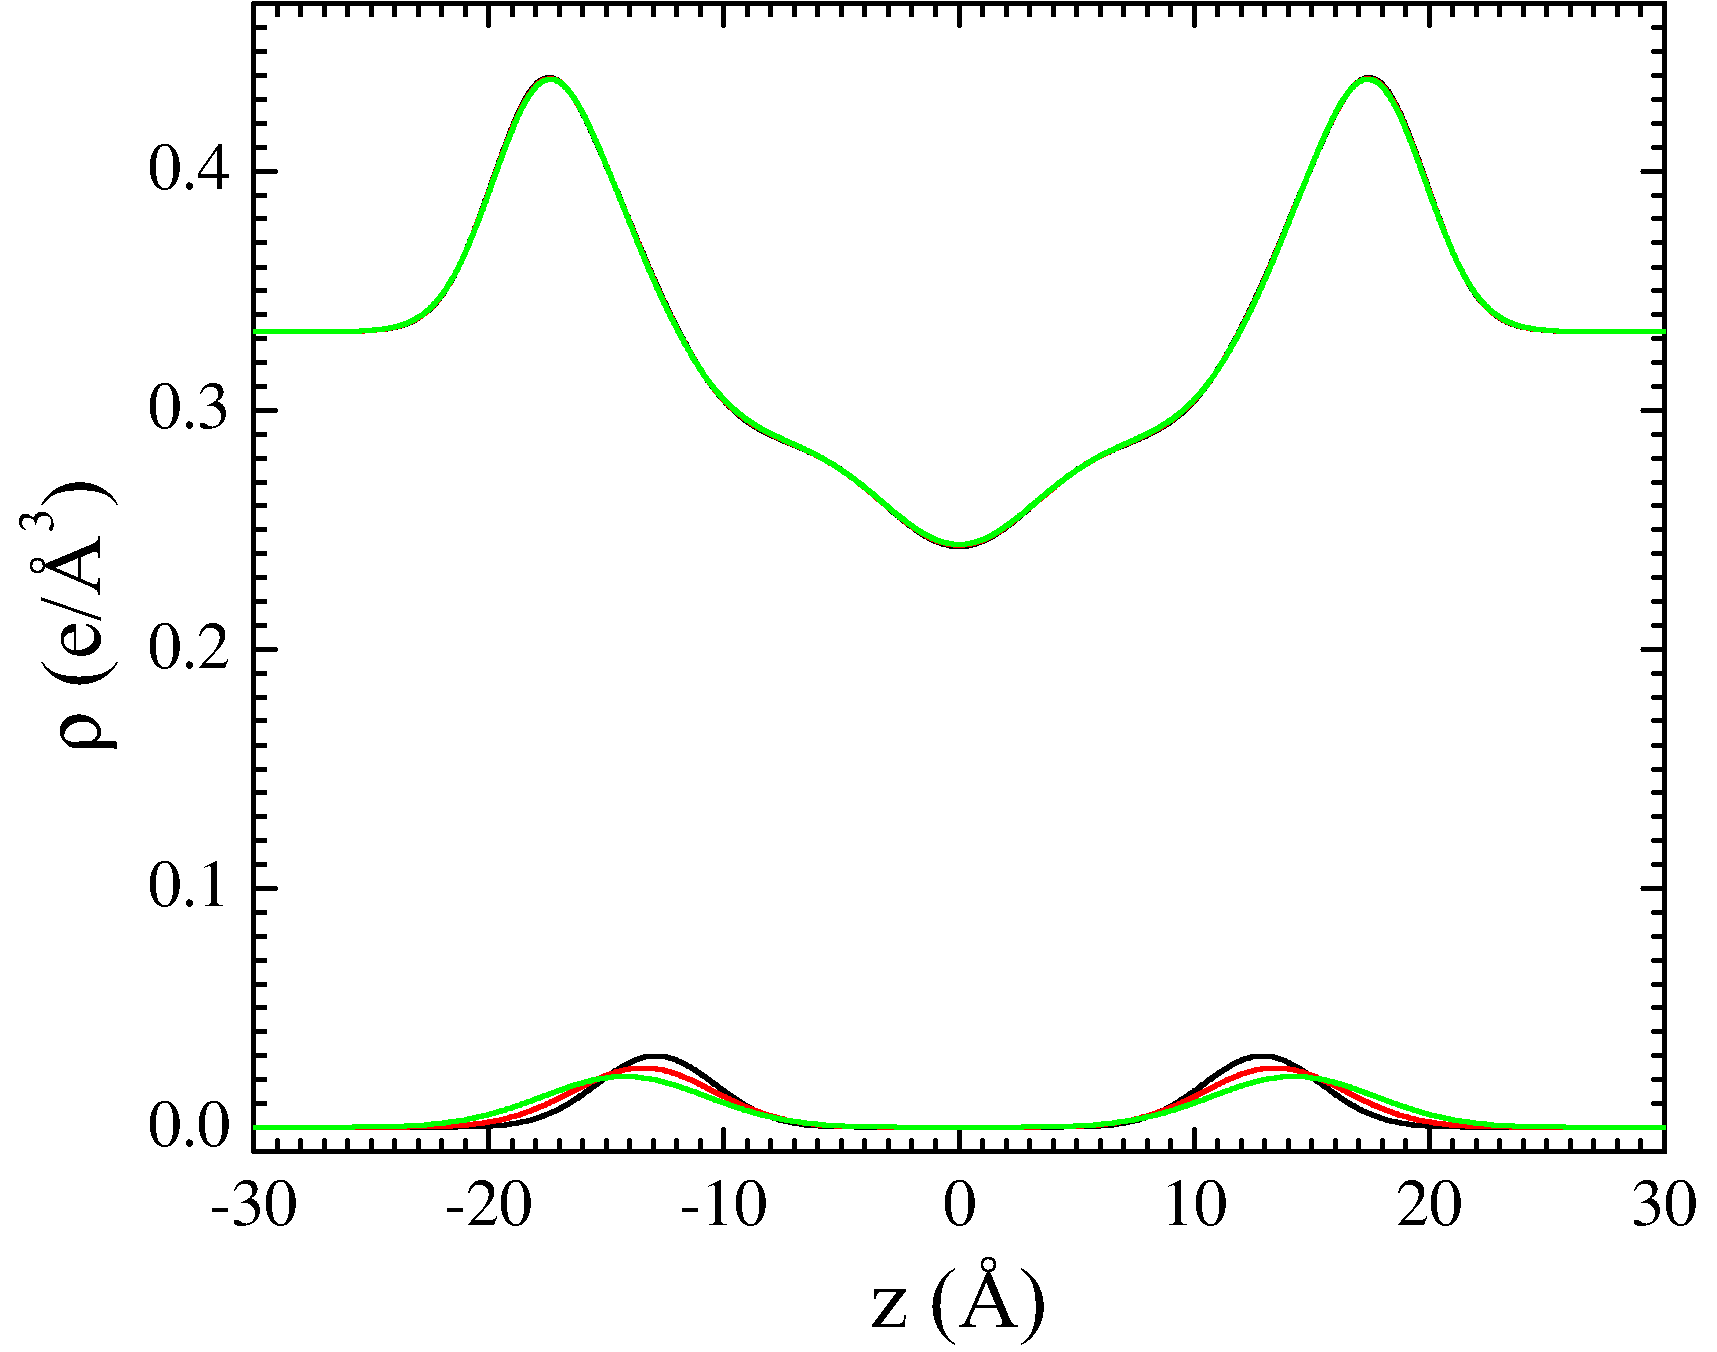
\includegraphics[width=0.5\textwidth]{figures/Tat/SDP_Results/EDP/DOPC_Tat_62to1_EDP}
  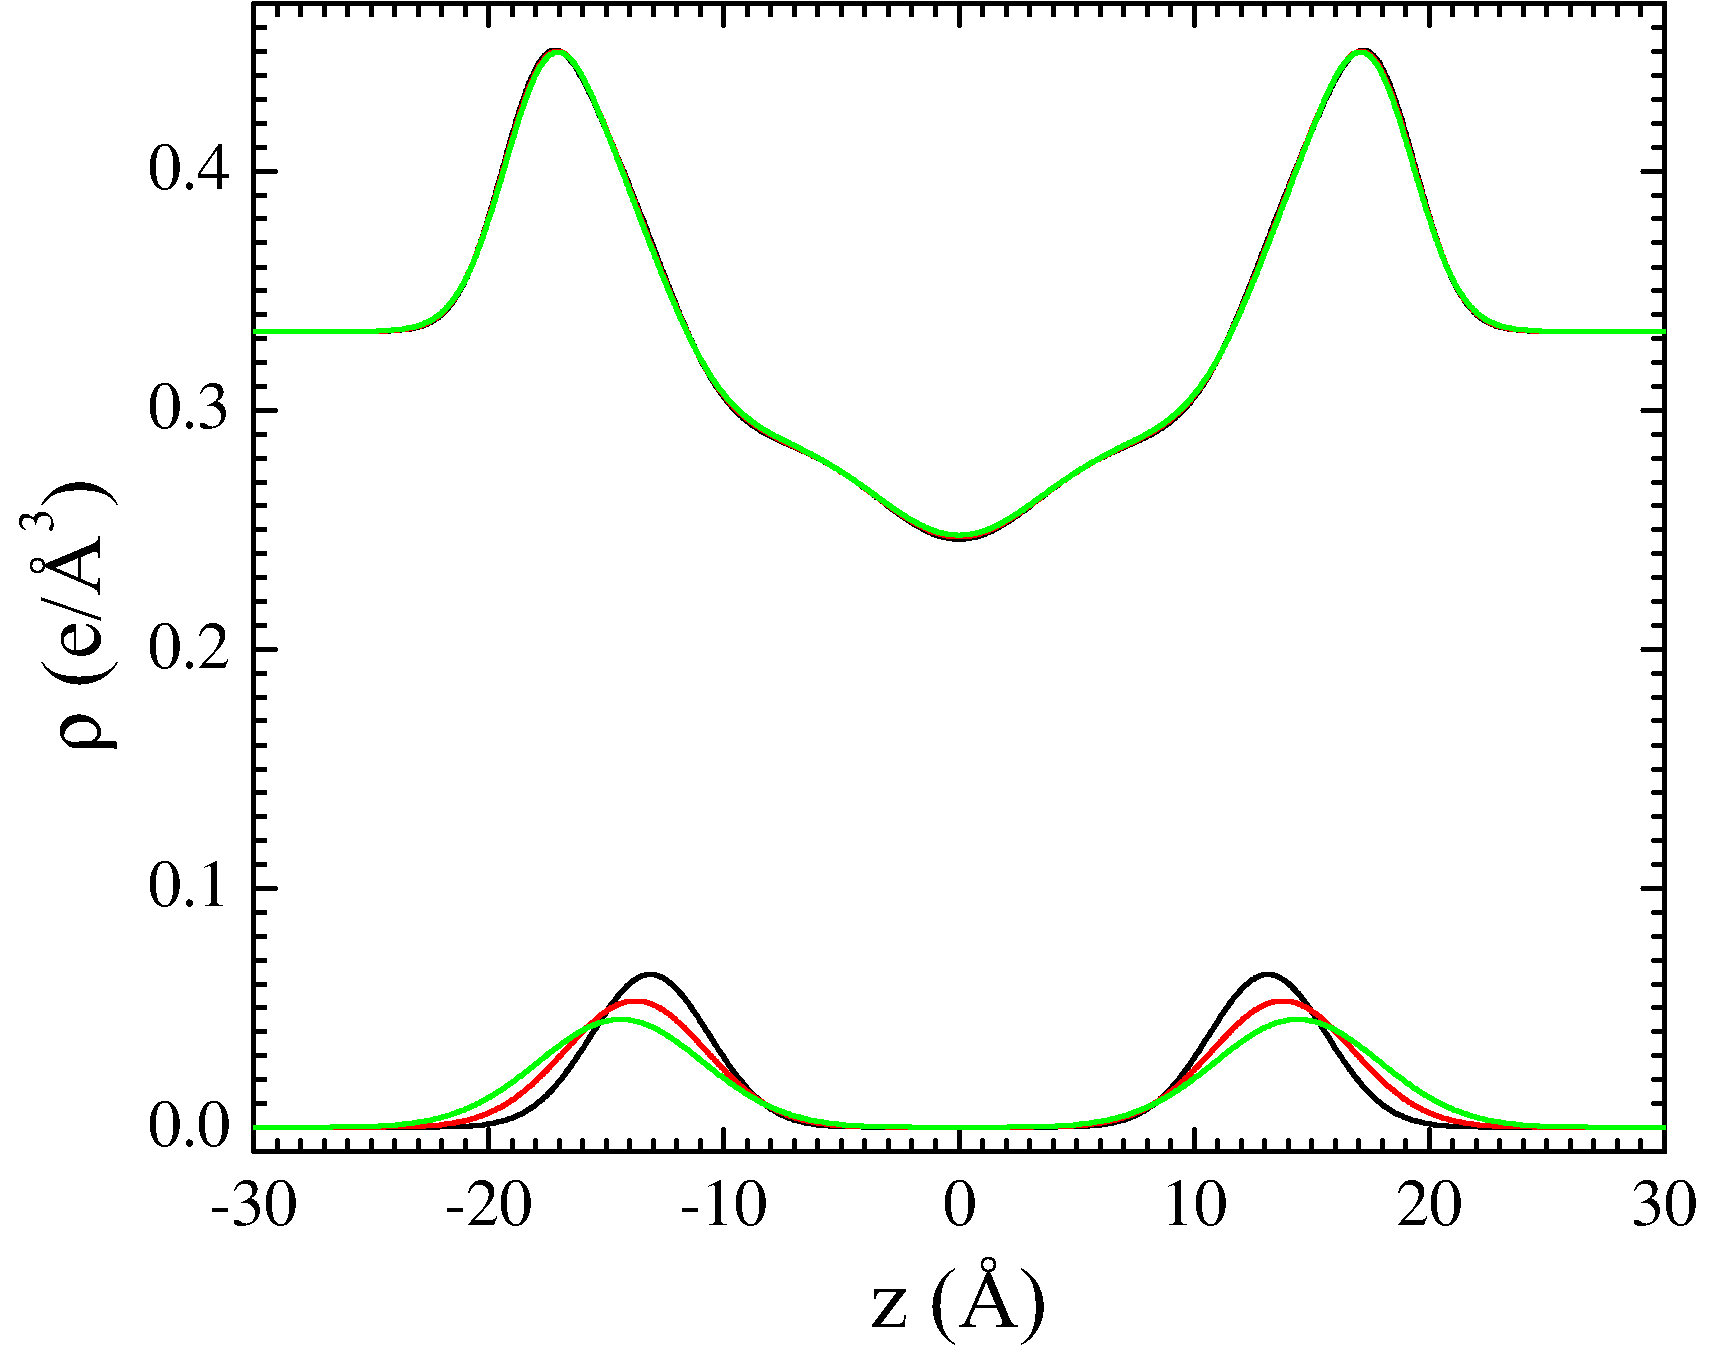
\includegraphics[width=0.5\textwidth]{figures/Tat/SDP_Results/EDP/DOPC_Tat_28to1_EDP}
  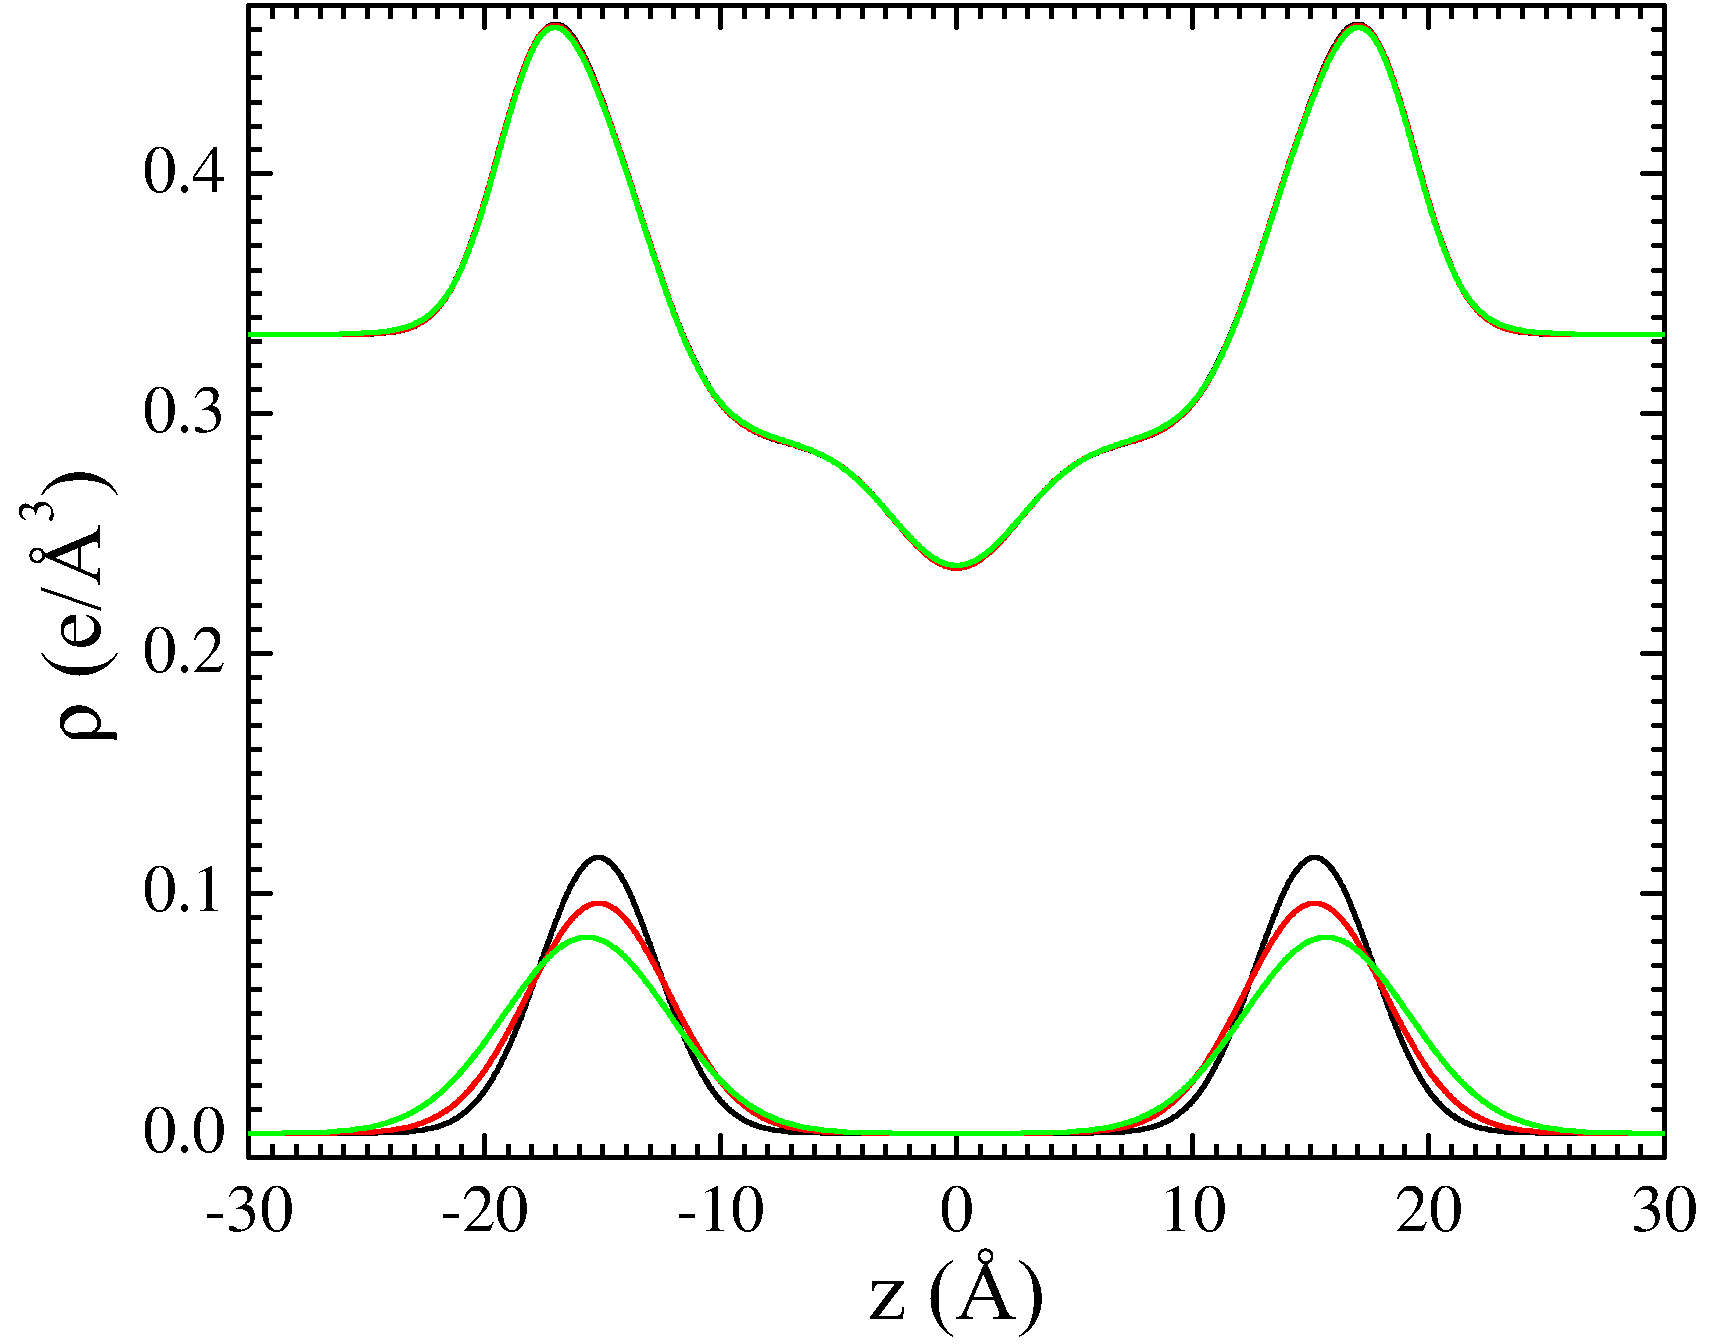
\includegraphics[width=0.5\textwidth]{figures/Tat/SDP_Results/EDP/DOPC_Tat_16to1_EDP}
  \caption[Comparison of total electron density profiles corresponding to best fits using 
  different Tat widths $\sigmaTat$, 2.5 (red), 3.0 (black), and 3.5 (green)]
  {Comparison of total electron density profiles corresponding to best fits using 
  different Tat widths $\sigmaTat$, 2.5 (red), 3.0 (black), and 3.5 (green). 
  The mole fraction of Tat $\xTat$
  was 0.016 (top), 0.034 (middle), and 0.059 (bottom). While different values of 
  $\sigmaTat$ resulted in different positions of Tat, the total electron density
  profiles were almost identical and independent of $\sigmaTat$.}
  \label{fig:DOPC_Tat_EDP}
\end{figure}

In contrast to $\DHH$, $\DPP$ is a property that
depends on lipid components, which are influenced by how the lipid is parsed 
(see Sec.~\ref{sec:SDP_method})
and what assumptions and constraints go into the specific model.
A disadvantage of using $\DHH$ as a measure of the membrane thickness is
that $\DHH$ is influenced by the electron density of Tat because 
the total electron density profile includes a contribution from the electron density of Tat. 
Especially when the mole fraction of Tat in a system becomes large, 
the Tat electron density contributes significantly to the total electron 
density profile. If Tat resided slightly 
outside of the PC component, the apparent membrane thickness measured by $\DHH$
would be larger than $\DPP$. Then, even if the actual bilayer thickness defined by $\DPP$ 
were reduced by the presence of Tat, the effect of thinning might not be obvious. 

As described in the previous paragraph, the model parameters were sensitive to 
specific constraints and assumptions on the model, and as Fig.~\ref{fig:DOPC_Tat_EDP}
shows, the position of Tat depended on $\sigmaTat$. On the other hand,
the total electron density profiles were seen to be less sensitive. 
Figure~\ref{fig:DOPC_Tat_total_EDP} compares the total electron density profiles
at different Tat concentrations. Consistent with the form factors shifting 
to larger $q_z$ as $\xTat$ increased, $\DHH$ decreased as $\xTat$ increased.
As argued earlier, a decrease in $\DHH$ does not necessarily indicate a decrease
in the bilayer thickness, and it could instead be attributed to deeper insertion
of Tat into the bilayer. However, compared to the profile of DOPC alone,
all three profiles with Tat deviate from the electron density of water 
at smaller $|z|$ when approached from the water region. This is illustrated 
in Fig.~\ref{fig:DOPC_Tat_total_EDP_difference} that plots the difference 
between the total electron density profile of DOPC and those of DOPC with Tat.
Negative values of $\Delta\rho = \rho_\text{DOPC+Tat} - \rho_\text{DOPC}$
(the region labeled $\Delta\rho < 0$ in Fig.~\ref{fig:DOPC_Tat_total_EDP_difference})
indicate that the headgroup, which has excess electron density relative to
water, shifted toward the bilayer center as Tat was added to the system,
which implies bilayer thinning. This effect can also be seen in 
Fig.~\ref{fig:DOPC_Tat_total_EDP}.

\begin{figure}[htbp]
  \centering
  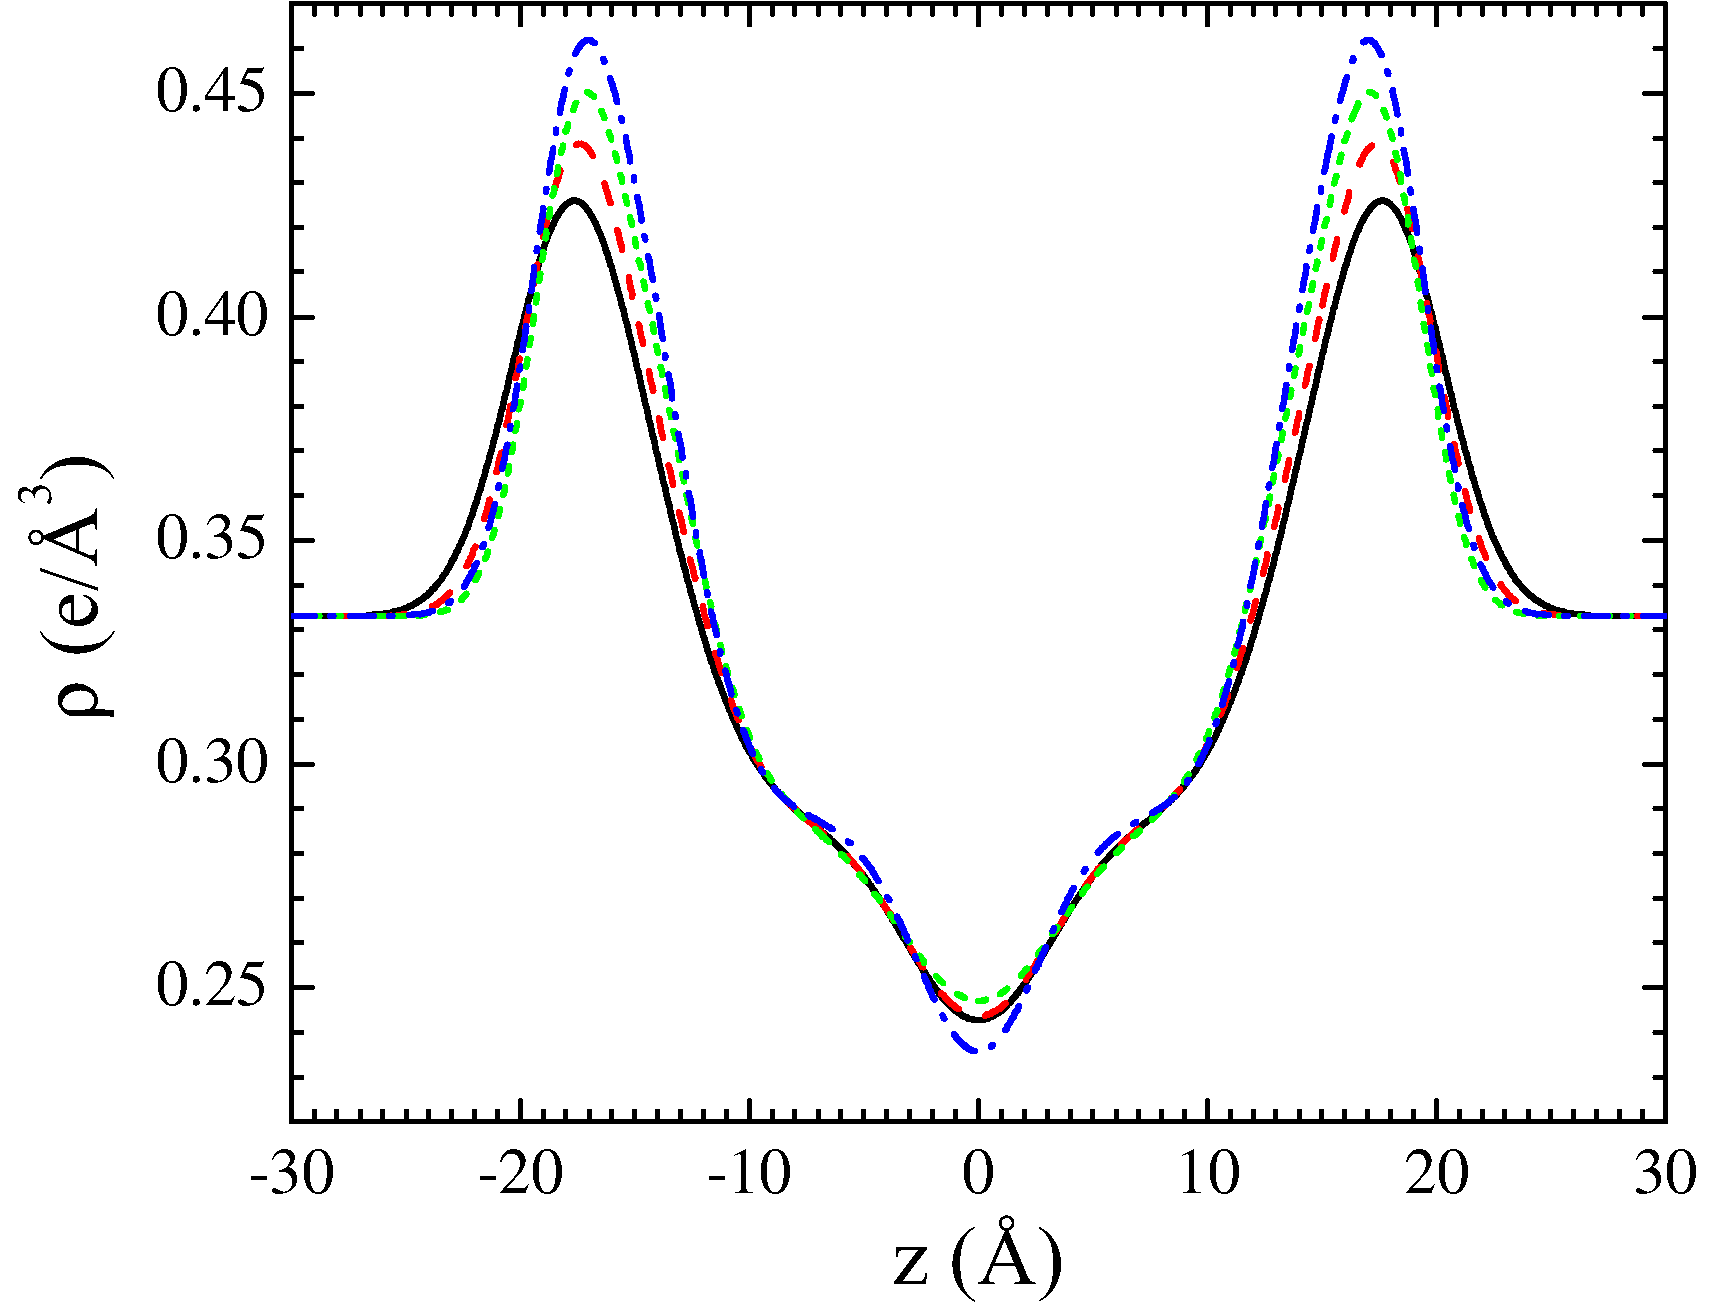
\includegraphics[width=0.7\textwidth]{figures/Tat/SDP_Results/EDP/DOPC_Tat_total_EDP}
  \caption[Comparison of DOPC total electron density profiles at $\xTat$ = 0 (black solid),
  0.016 (red dash), 0.034 (green short dash), and 0.059 (blue dash dot)]
  {Comparison of DOPC total electron density profiles at $\xTat$ = 0 (black solid),
  0.016 (red dash), 0.034 (green short dash), and 0.059 (blue dash dot).}
  \label{fig:DOPC_Tat_total_EDP}
\end{figure}

\begin{figure}[htbp]
  \centering
  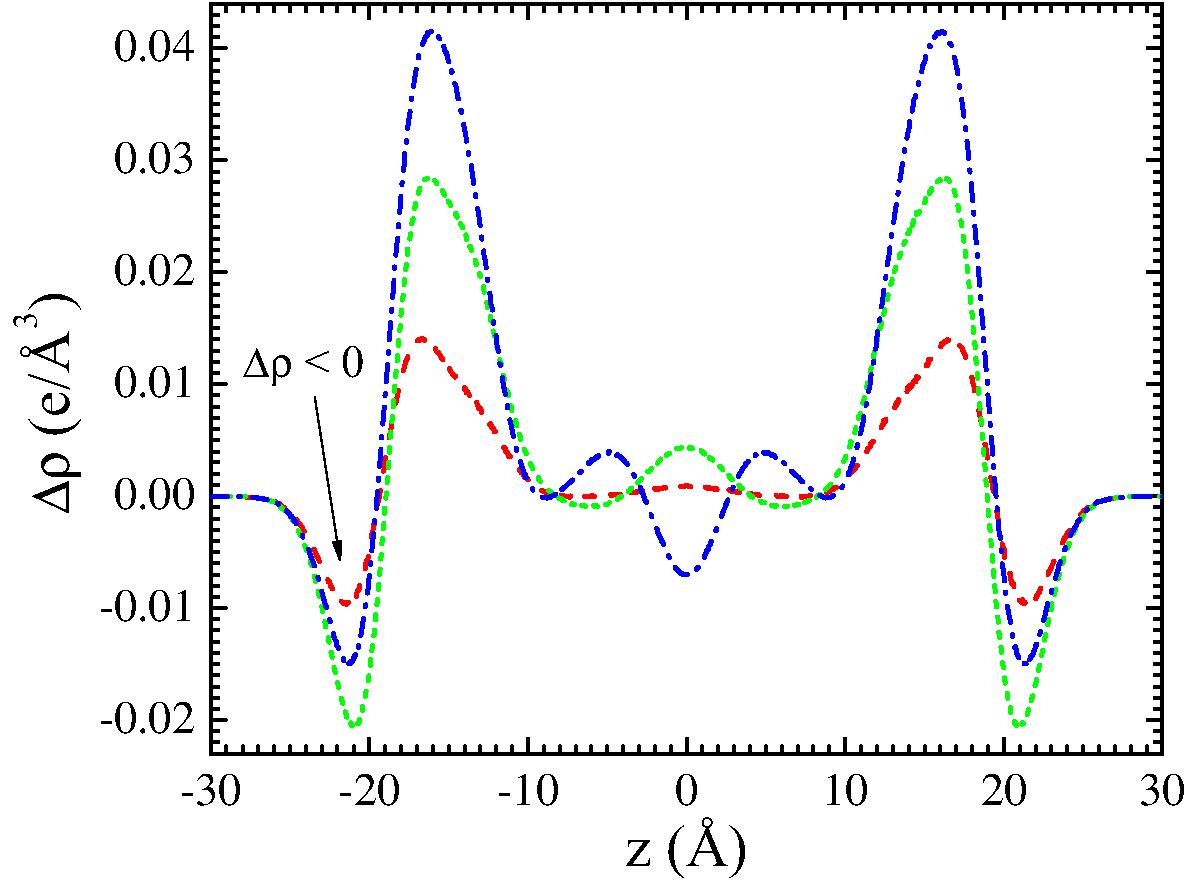
\includegraphics[width=0.7\textwidth]{figures/Tat/SDP_Results/EDP/DOPC_Tat_total_EDP_diff}
  \caption[Difference between total electron density profiles of DOPC with Tat 
  and that of DOPC $\Delta\rho = \rho_\text{DOPC+Tat} - \rho_\text{DOPC}$]
  {Difference between total electron density profiles of DOPC with Tat 
  and that of DOPC $\Delta\rho = \rho_\text{DOPC+Tat} - \rho_\text{DOPC}$. 
  $\xTat$ = 0.016 (red dash), 0.034 (green short dash), 
  and 0.059 (blue dash dot). Positive $\Delta\rho$ means excess electron density 
  due to presence of Tat. The region labeled $\Delta\rho < 0$ indicates that 
  the electron dense headgroup moved closer to the bilayer center upon addition of Tat,
  which is equivalent to bilayer thinning.}
  \label{fig:DOPC_Tat_total_EDP_difference}
\end{figure}

Fitting results for DOPC:DOPE (3:1) and DOPC:DOPE (1:1) are summarized 
in Table~\ref{tab:DOPCDOPE3to1_fit_results} and 
Table~\ref{tab:DOPCDOPE1to1_fit_results}, respectively,
and the best fits and corresponding electron density profiles are shown in 
Fig.~\ref{fig:DOPCDOPE3to1_Tat_XFF1} and Fig.~\ref{fig:DOPCDOPE1to1_Tat_XFF1}
at the end of this subsection. 
Figure~\ref{fig:DOPCDOPE_Tat_total_EDP} plots total electron density profiles,
showing increasing electron density in the headgroup region as Tat concentration
increased, similarly to DOPC/Tat systems shown in Fig.~\ref{fig:DOPC_Tat_total_EDP}.

\begin{table}[htbp]
  \centering
  \begin{tabular}{c|c|ccc|ccc|ccc}
    \hline
    $\xTat$ & 0 & 0.016 & 0.016 & 0.016 & 0.034 & 0.034 & 0.034 & 0.059 & 0.059 & 0.059 \\
    \hline
    $\chi^2$ & 924.5 & {\color{red}4972} & 4985 & 4994 & {\color{red}6758} & 6826 & 6863 & 2293 & {\color{red}2280} & 2296 \\ 
    $\zPC$ & 18.3 & 18.5 & 18.5 & 18.4 & 18.5 & 18.4 & 18.3 & 18.2 & 18.2 & 18.1 \\
    $\sigmaPC$ & 2.66 & 2.23 & 2.26 & 2.27 & 2.25 & 2.31 & 2.34 & 2.31 & 2.19 & 2.11 \\
    $\zCG$ & 15.2 & 15.4 & 15.4 & 15.3 & 15.4 & 15.3 & 15.2 & 15.1 & 15.1 & 15.0 \\
    $\sigmaCG$ & 2.92 & 2.63 & 2.65 & 2.69 & 2.52 & 2.58 & 2.63 & 2.40 & 2.20 & 2.01 \\
    $\zHC$ & 13.9 & 14.1 & 14.1 & 14.0 & 14.1 & 14.0 & 13.9 & 13.8 & 13.8 & 13.7 \\
    $\sigmaHC$ & 2.73 & 2.70 & 2.83 & 2.91 & 2.86 & 2.79 & 2.84 & 2.25 & 2.38 & 2.60 \\
    $\sigmaCHthree$ & 3.24 & 2.94 & 2.97 & 2.98 & 2.87 & 2.90 & 2.91 & 2.63 & 2.61 & 2.65 \\
    $\zTat$ & NA & 13.5 & 14.0 & 15.0 & 14.3 & 14.9 & 16.0 & 16.3 & 16.4 & 16.9 \\
    $\sigmaTat$ & NA & 2.5 & 3.0 & 3.5 & 2.5 & 3.0 & 3.5 & 2.5 & 3.0 & 3.5 \\ 
    $\AL$ & 70.9 & 69.8 & 69.9 & 70.1 & 69.5 & 70.0 & 70.6 & 71.3 & 71.4 & 71.7 \\
    \hline
  \end{tabular}
  \caption[Fitting Results for DOPC:DOPE (3:1) membranes for the THG model]
  {Fitting Results for DOPC:DOPE (3:1) membranes for the THG model. 
  The smallest $\chi^2$ values at each Tat mole fraction $\xTat$ are highlighted in red.  
  $\zPC-\zCG = 3.1$ \AA\ and $\zCG-\zHC = 1.3$ \AA\ in all fits.
  Units of all symbols are \AA\ except for $\chi^2$ (unitless) and $\AL$ (\AA$^2$).}
  \label{tab:DOPCDOPE3to1_fit_results}
\end{table}

\begin{table}[htbp]
  \centering
  \begin{tabular}{c|c|ccc|ccc|ccc}
    \hline
    $\xTat$ & 0 & 0.016 & 0.016 & 0.016 & 0.034 & 0.034 & 0.034 & 0.059 & 0.059 & 0.059 \\
    \hline
    $\chi^2$ & 2961 & {\color{red}1554} & 1570 & 1581 & {\color{red}1563} & 1587 & 1607 & 2342 & {\color{red}2338} & 2363 \\     
    $\zPC$ & 18.1 & 18.0 & 17.9 & 17.9 & 17.8 & 17.7 & 17.6 & 17.8 & 17.8 & 17.7 \\
    $\sigmaPC$ & 2.52 & 2.14 & 2.17 & 2.18 & 1.86 & 1.92 & 1.93 & 2.02 & 1.97 & 1.93 \\
    $\zCG$ & 15.0 & 14.9 & 14.8 & 14.8 & 14.7 & 14.6 & 14.5 & 14.7 & 14.7 & 14.6 \\
    $\sigmaCG$ & 3.00 & 2.62 & 2.64 & 2.66 & 2.22 & 2.30 & 2.31 & 2.58 & 2.27 & 2.14 \\
    $\zHC$ & 13.7 & 13.6 & 13.5 & 13.5 & 13.4 & 13.3 & 13.2 & 13.4 & 13.4 & 13.3 \\ 
    $\sigmaHC$ & 3.00 & 2.69 & 2.84 & 2.95 & 2.65 & 2.82 & 3.01 & 2.47 & 2.58 & 2.83 \\
    $\sigmaCHthree$ & 3.20 & 3.19 & 3.22 & 3.24 & 3.37 & 3.43 & 3.47 & 2.70 & 2.70 & 2.74 \\
    $\zTat$ & NA & 12.9 & 13.4 & 14.2 & 13.1 & 13.8 & 14.4 & 15.2 & 15.2 & 15.7 \\
    $\sigmaTat$ & NA & 2.5 & 3.0 & 3.5 & 2.5 & 3.0 & 3.5 & 2.5 & 3.0 & 3.5 \\ 
    $\AL$ & 71.5 & 72.4 & 72.5 & 72.7 & 73.6 & 74.0 & 74.4 & 73.6 & 73.5 & 73.9 \\
    \hline
  \end{tabular}
  \caption[Fitting Results for DOPC:DOPE (1:1) membranes for the THG model]
  {Fitting Results for DOPC:DOPE (1:1) membranes for the THG model. 
  The smallest $\chi^2$ values at each Tat mole fraction $\xTat$ are highlighted in red.
  $\zPC-\zCG = 3.1$ \AA\ and $\zCG-\zHC = 1.3$ \AA\ in all fits.
  Units of all symbols are \AA\ except for $\chi^2$ (unitless) and $\AL$ (\AA$^2$).}
  \label{tab:DOPCDOPE1to1_fit_results}
\end{table}

\begin{figure}[htbp]
  \centering
  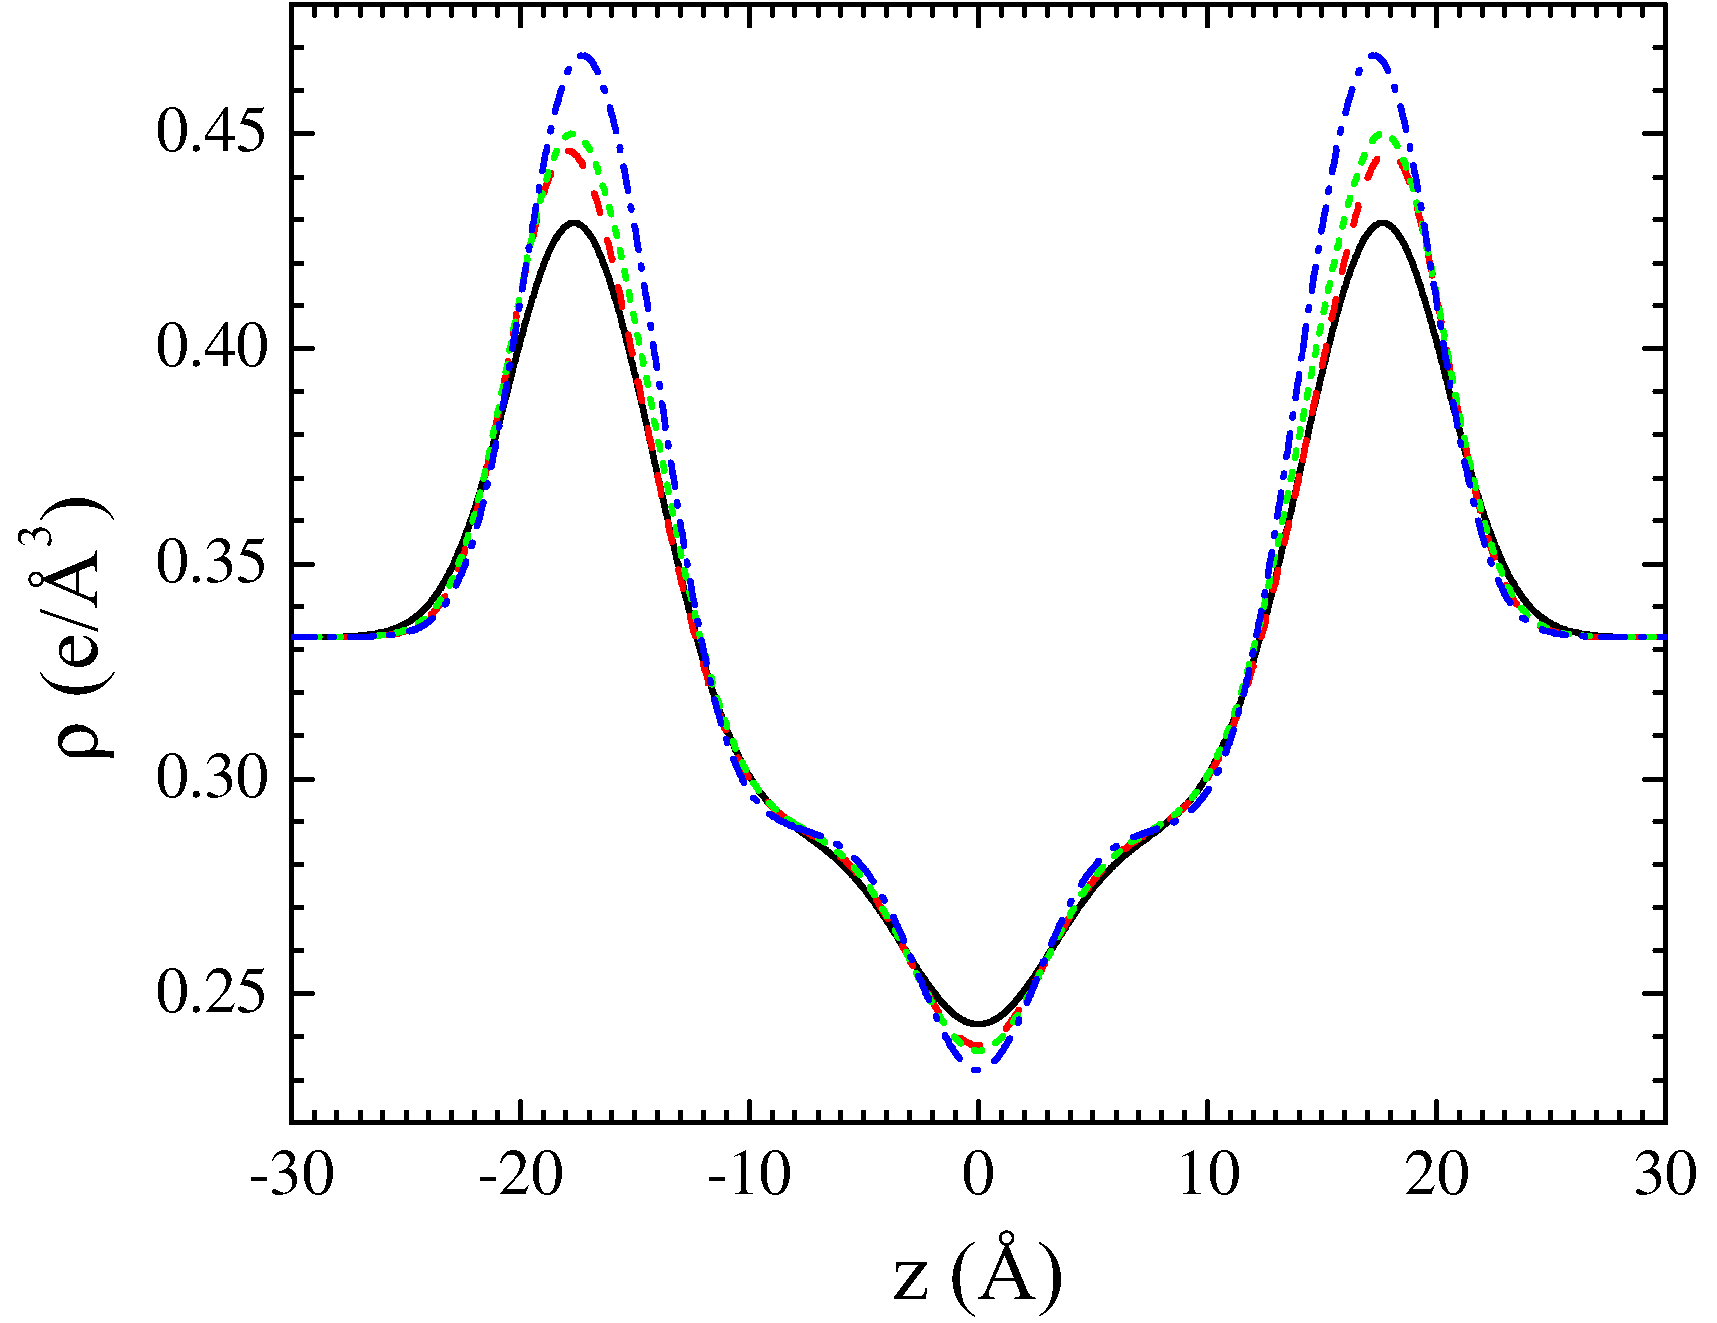
\includegraphics[width=0.45\textwidth]{figures/Tat/SDP_Results/EDP/DOPCDOPE3to1_Tat_total_EDP}
  \qquad
  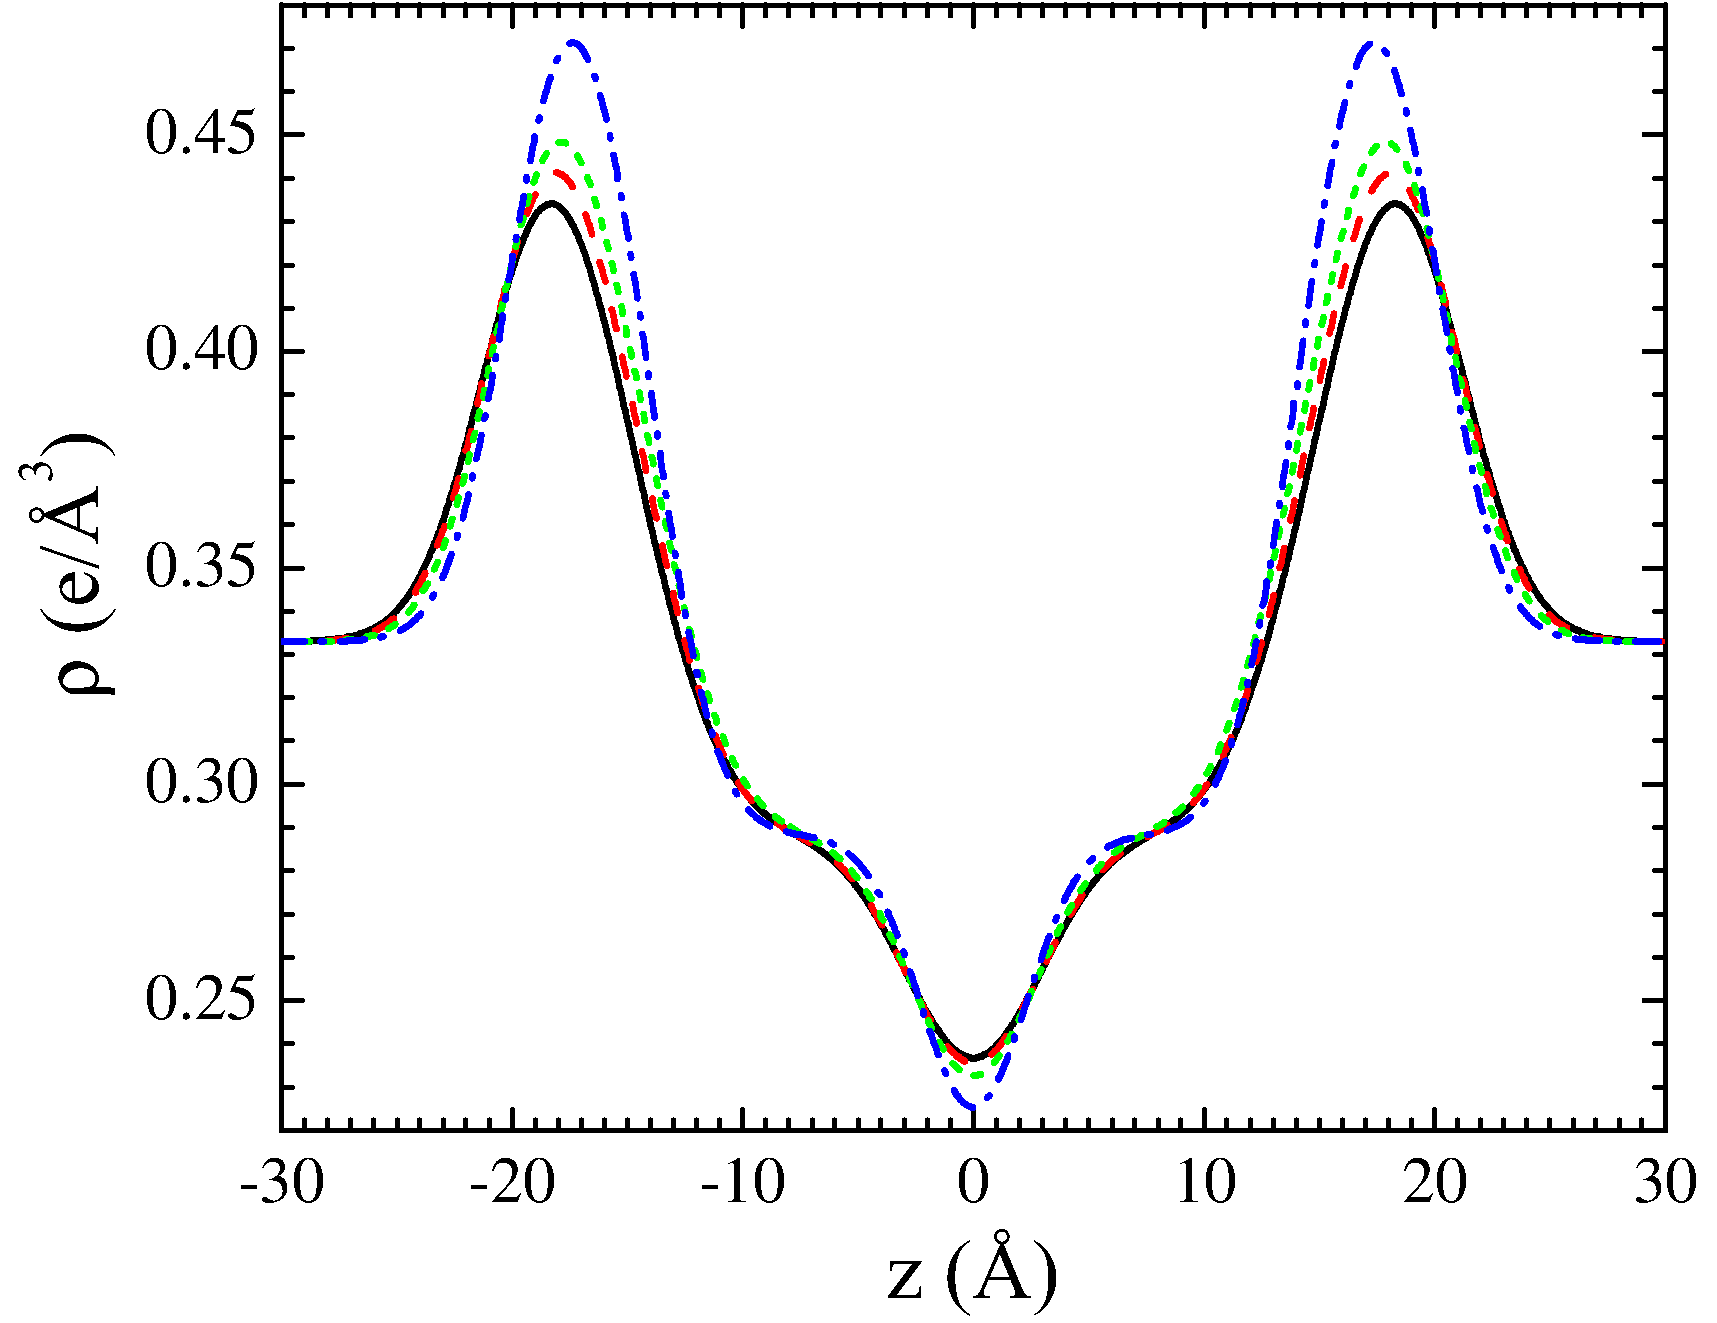
\includegraphics[width=0.45\textwidth]{figures/Tat/SDP_Results/EDP/DOPCDOPE1to1_Tat_total_EDP}
  \caption[Total electron density profiles for DOPC:DOPE (3:1) (left) and 
  DOPC:DOPE (1:1) (right) with Tat mole fraction $\xTat$ = 0 (black solid),
  0.016 (red dash), 0.034 (green short dash), and 0.059 (blue dash dot)]
  {Total electron density profiles for DOPC:DOPE (3:1) (left) and 
  DOPC:DOPE (1:1) (right) with Tat mole fraction $\xTat$ = 0 (black solid),
  0.016 (red dash), 0.034 (green short dash), and 0.059 (blue dash dot).}
  \label{fig:DOPCDOPE_Tat_total_EDP}
\end{figure}

Figure~\ref{fig:DHH_DPP} summarizes the results for bilayer thickness as a function
of Tat mole fraction $\xTat$. In all cases, $\DHH$ was smaller than $\DPP$, consistent
with the results that the value of Tat position $\zTat$ was smaller 
than that of PC headgroup position $\zPC$. The CG headgroup also carries 
high average electron density and is located closer to the bilayer center than
the PC headgroup. Therefore, in general, $\DHH$ is smaller than $\DPP$ even
without Tat. Figure~\ref{fig:DPP_2zTat} compares Tat position 
to the PC headgroup position, reemphasizing the result that Tat is located
inside the PC headgroup. We note, however, that $\DPP$ in our models is
the average PC-PC distance and not necessarily the same as local bilayer 
thickness near a Tat peptide. It is reasonable to expect that the perturbation
of bilayer structure due to Tat is largest near Tat and decays as a
function of lateral distance from Tat. In Sec.~\ref{sec:MD_results}, we 
discuss local perturbation of a DOPC bilayer measured in MD simulations.
Finally, Fig.~\ref{fig:AL} plots area per lipid as a function of Tat mole
fraction. Consistent with bilayer thinning, area per lipid was found to 
increase in most cases. 
We could not obtain electron density profiles for DOPC:DOPS (3:1) and the nuclear membrane 
mimic, due to insufficient diffuse X-ray scattering by Tat charge neutralization 
of these negatively charged membranes, which rendered extraction of 
X-ray form factors unreliable.

\begin{figure}[htbp]
  \centering
  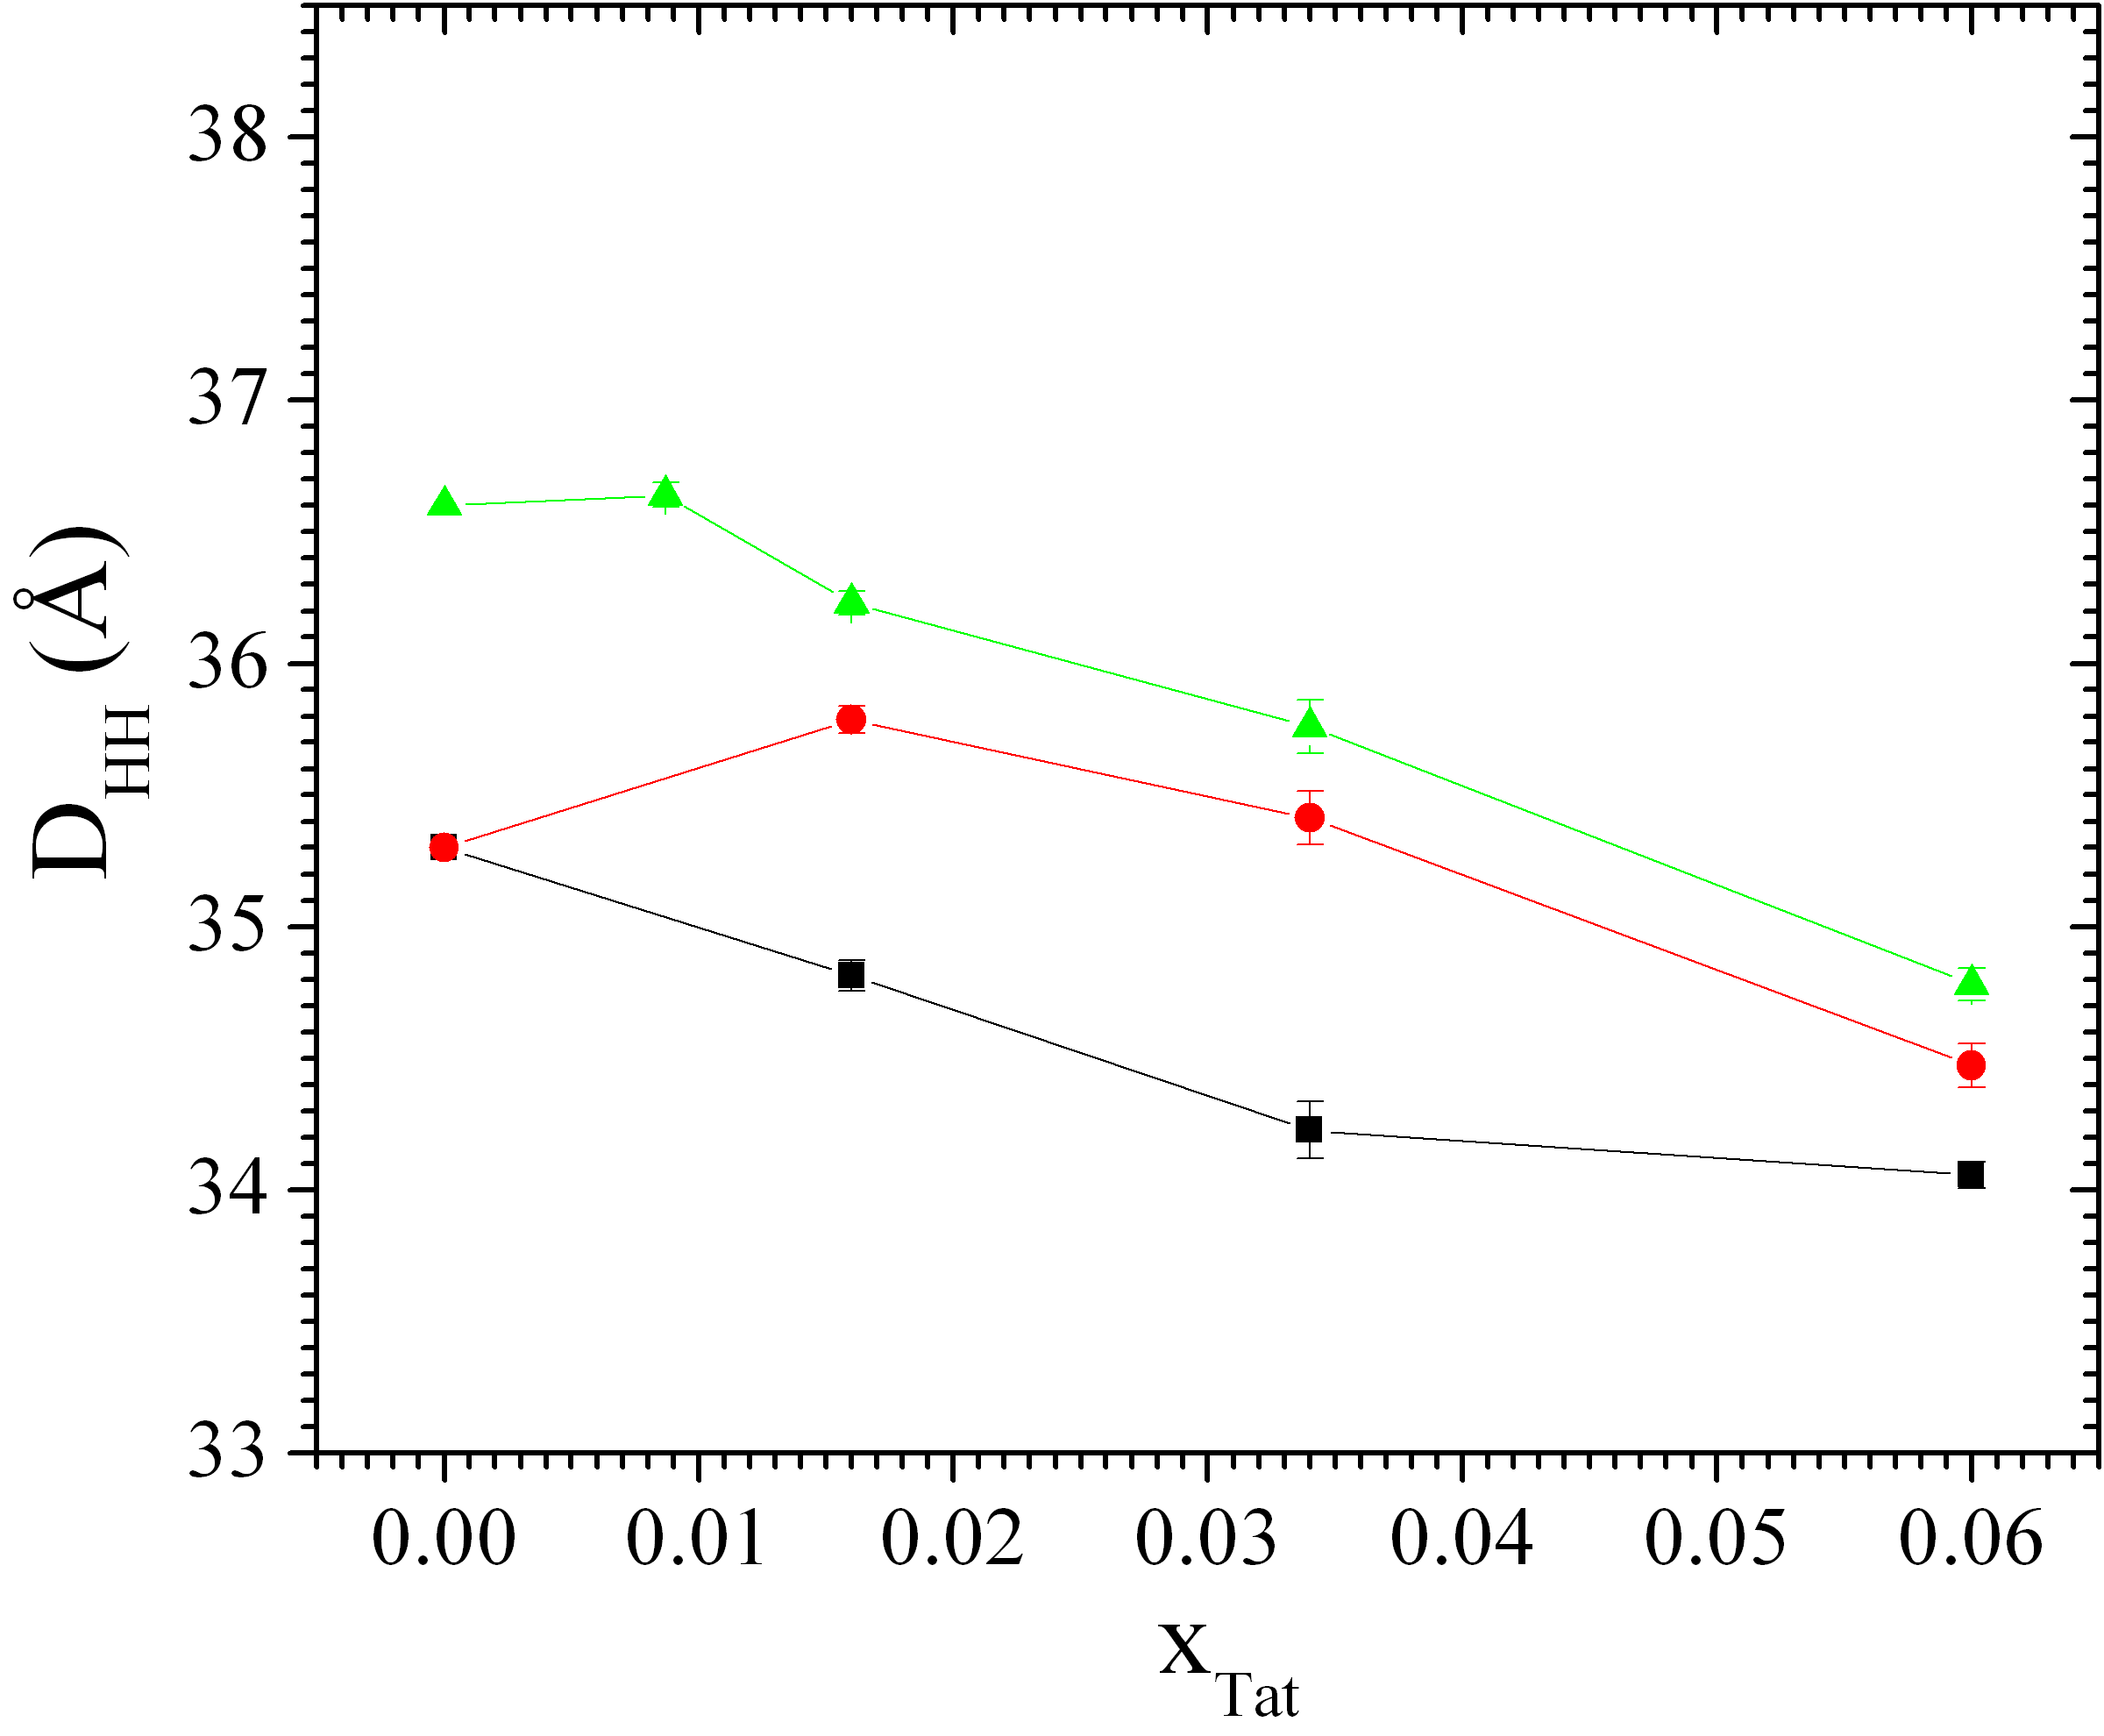
\includegraphics[width=0.45\textwidth]{figures/Tat/SDP_Results/DHH}
  \qquad
  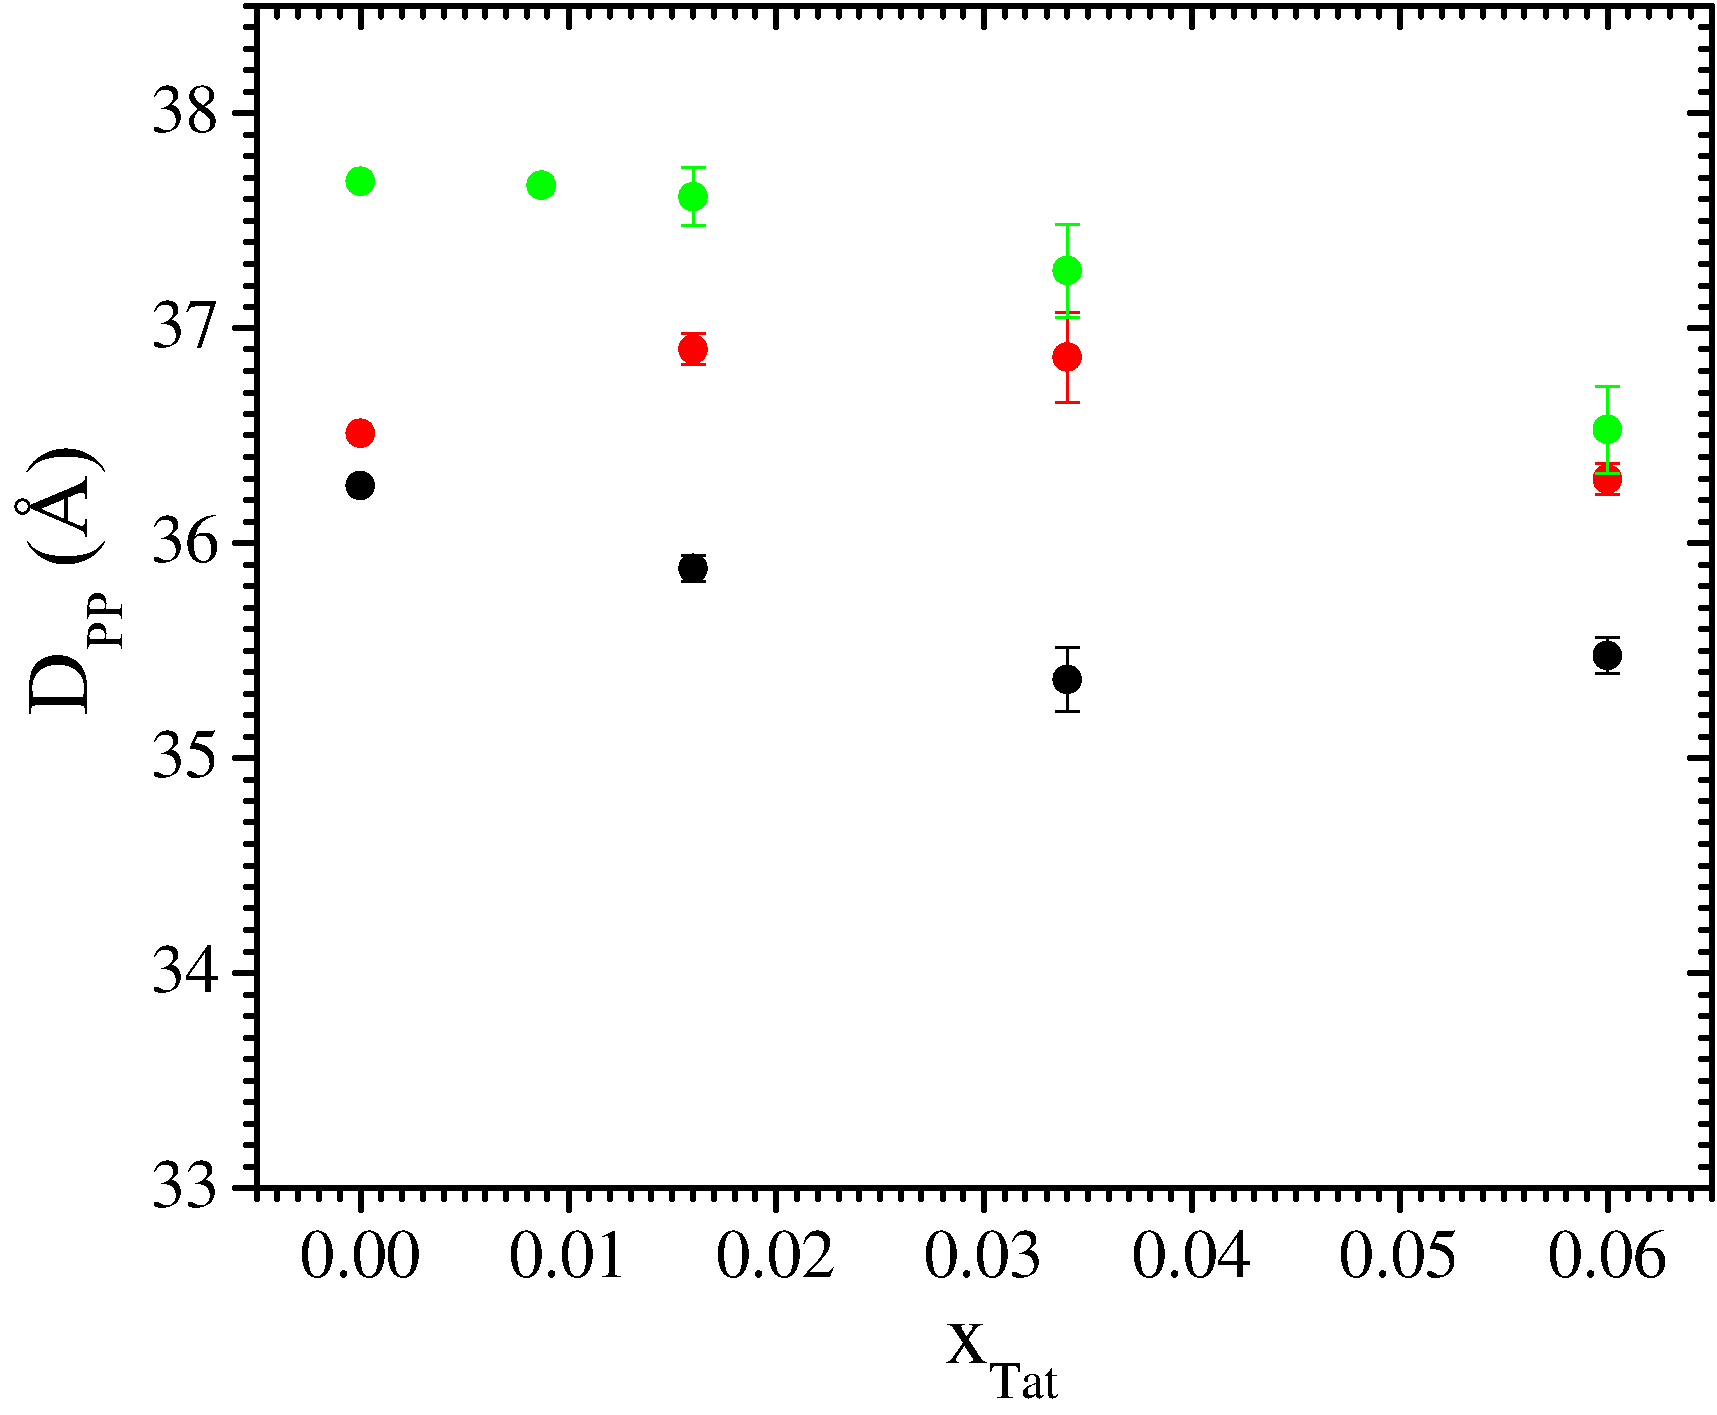
\includegraphics[width=0.45\textwidth]{figures/Tat/SDP_Results/DPP}
  \caption[Bilayer thickness, $\DHH$ (left) and $\DPP$ (right)
  plotted against Tat mole fraction $\xTat$]
  {Bilayer thickness, $\DHH$ (left) and $\DPP$ (right)
  plotted against Tat mole fraction $\xTat$.
  Black squares (DOPC), red circles (DOPC:DOPE (3:1)), and green
  triangles (DOPC:DOPE (1:1)).
  Error bars are standard deviations from imposing Tat Gaussian widths, 
  $\sigmaTat$ = 2.5, 3.0 or 3.5 \AA.}
  \label{fig:DHH_DPP}
\end{figure}

\begin{figure}[htbp]
  \centering
  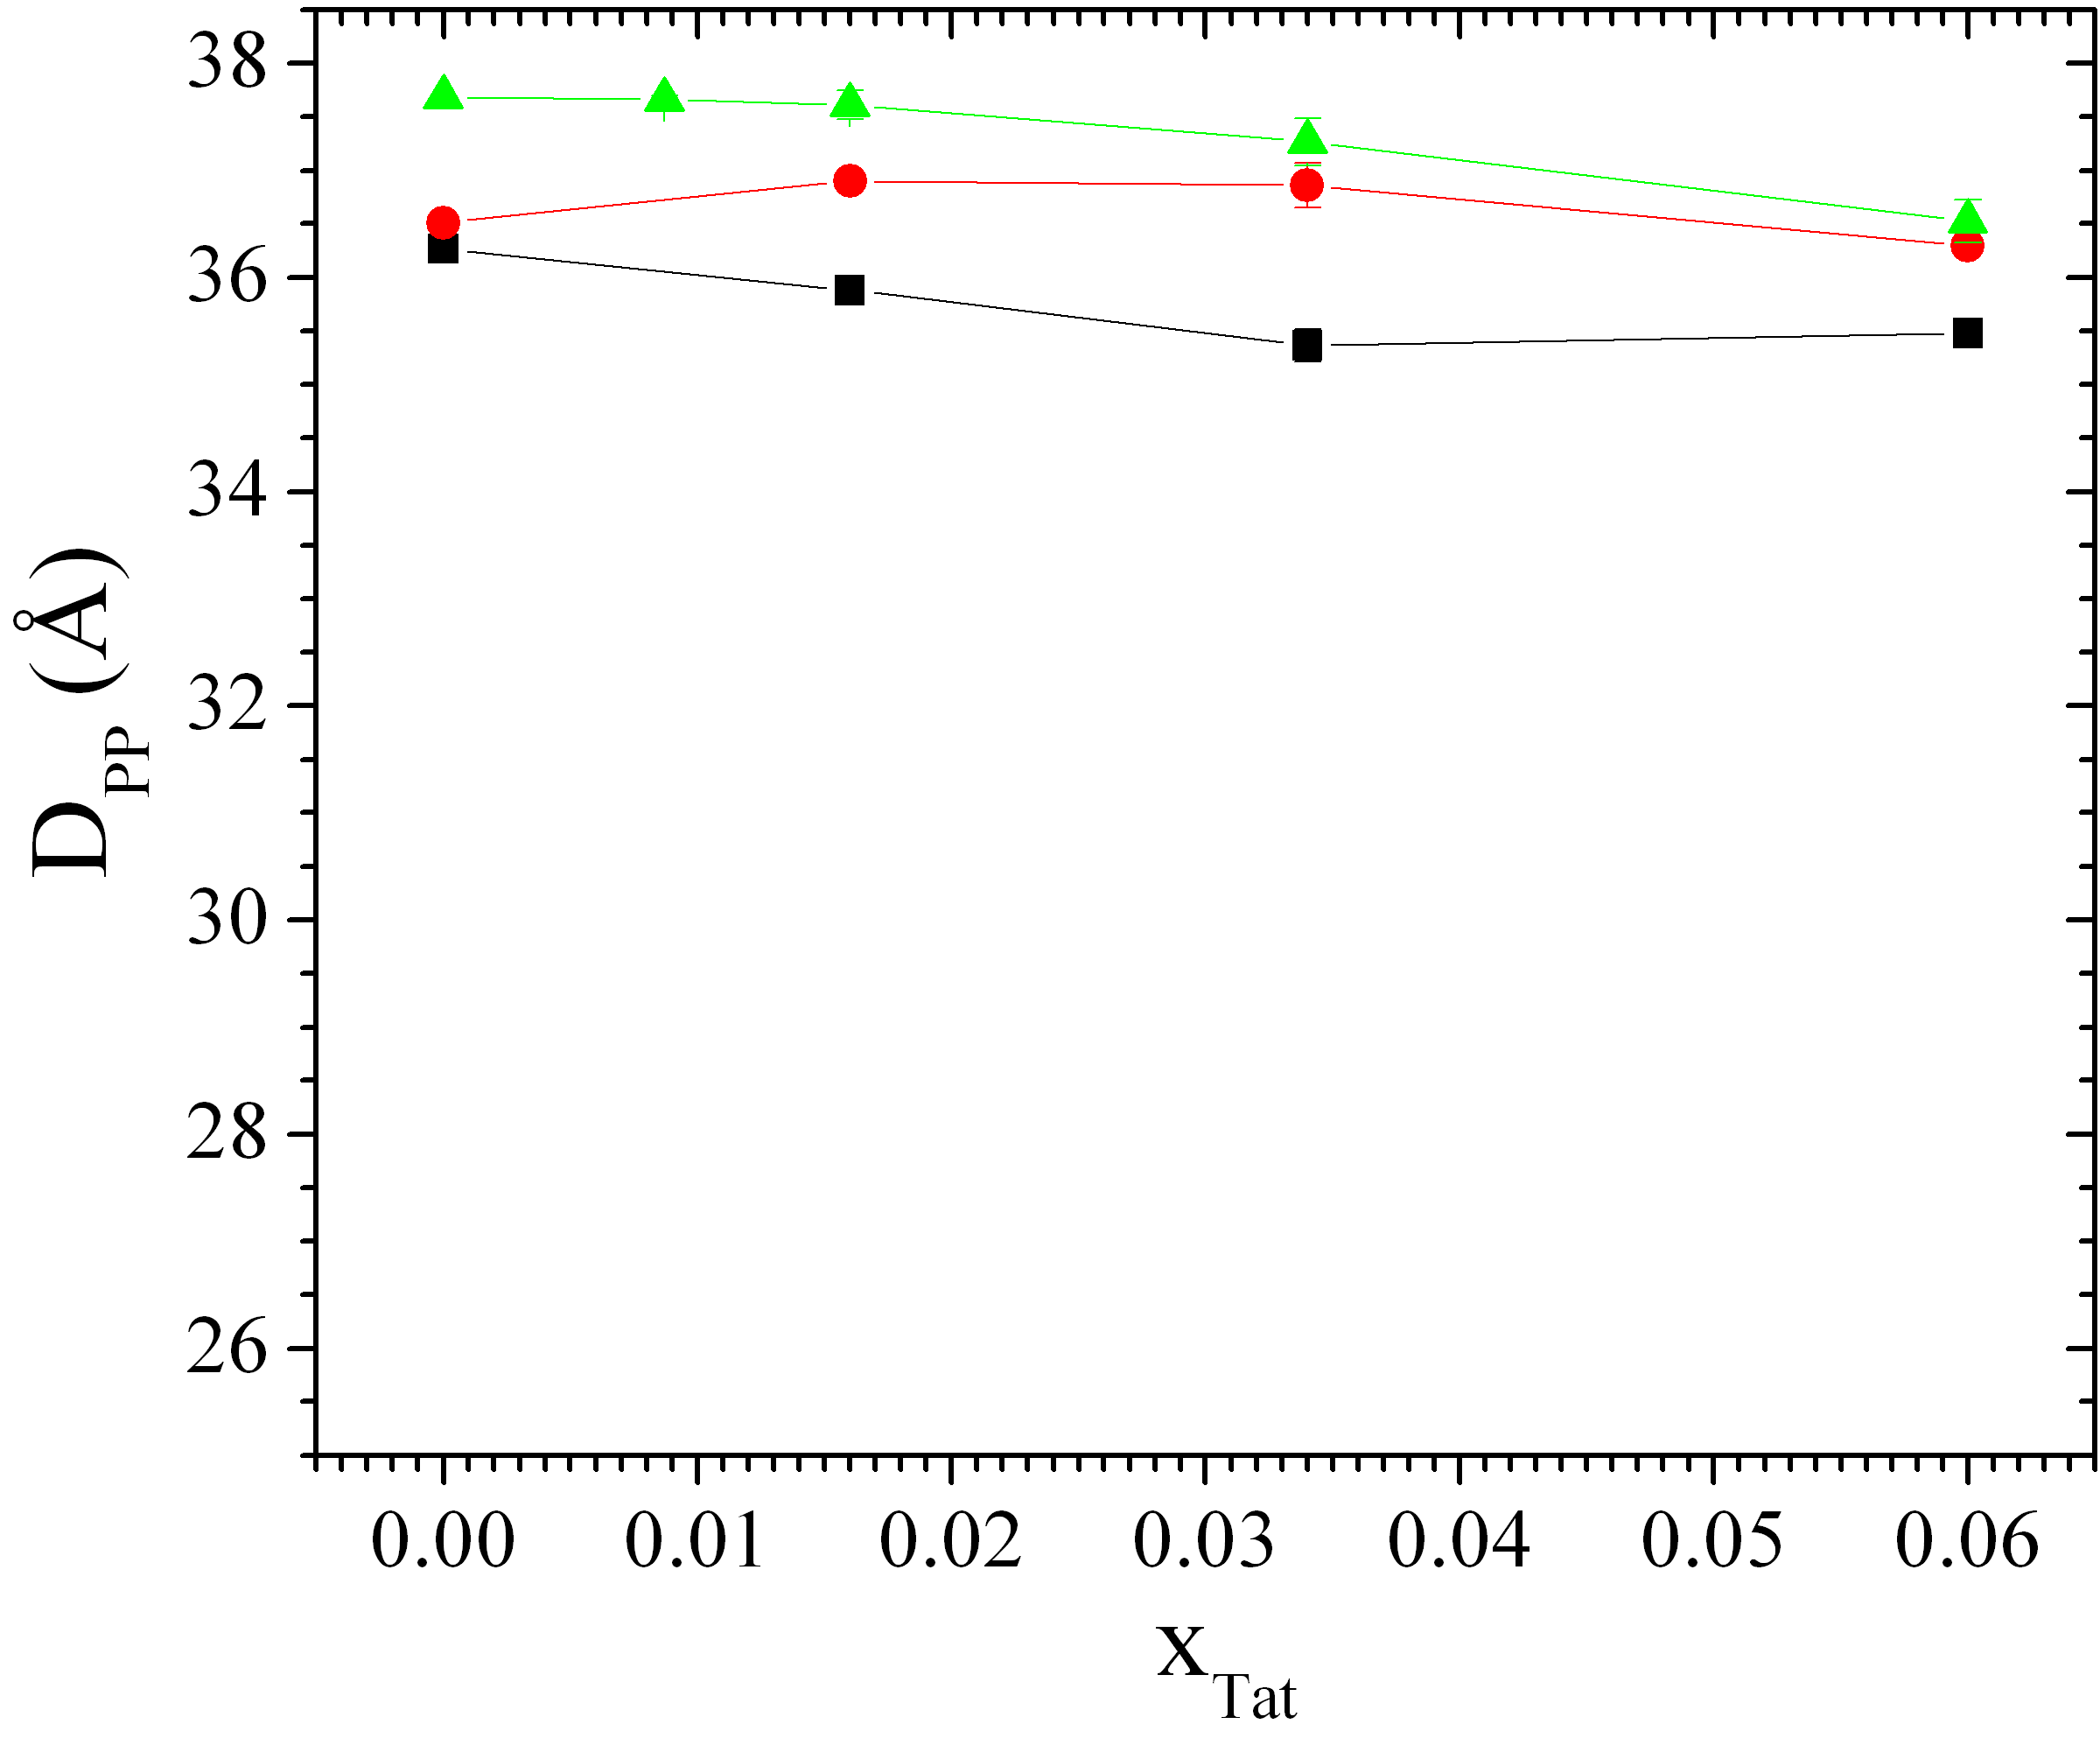
\includegraphics[width=0.45\textwidth]{figures/Tat/SDP_Results/DPP2}
  \qquad
  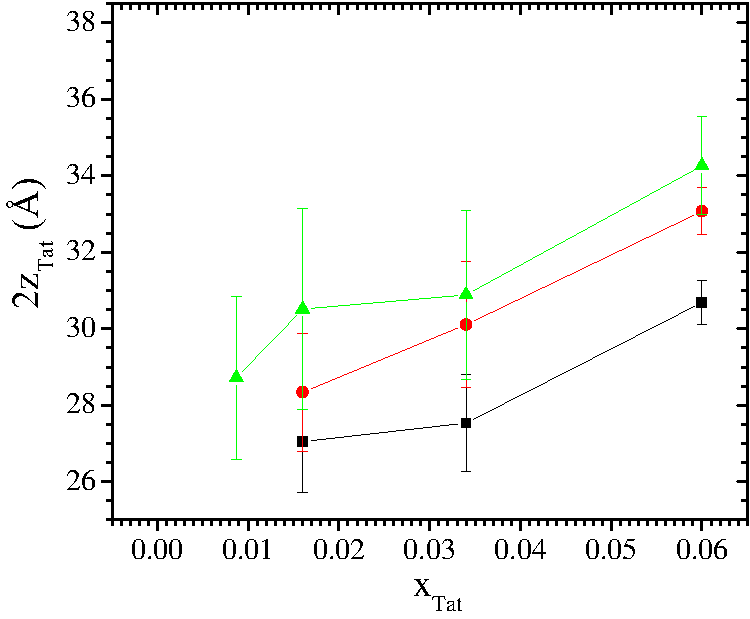
\includegraphics[width=0.45\textwidth]{figures/Tat/SDP_Results/2zTat}
  \caption[Bilayer thickness, $\DPP$ (left) and twice Tat position $2\zTat$ (right)
  plotted against Tat mole fraction $\xTat$]
  {Bilayer thickness, $\DPP$ (left) and twice Tat position $2\zTat$ (right)
  plotted against Tat mole fraction $\xTat$.
  Black squares (DOPC), red circles (DOPC:DOPE (3:1)), and green
  triangles (DOPC:DOPE (1:1)).
  Error bars are standard deviations from imposing Tat Gaussian widths, 
  $\sigmaTat$ = 2.5, 3.0 or 3.5 \AA. The data points of $\DPP$ (left) are 
  identical to those in Fig.~\ref{fig:DHH_DPP}, but the left axis is adjusted
  to facilitate comparison against $2\zTat$.}
  \label{fig:DPP_2zTat}
\end{figure}

\begin{figure}[htbp]
  \centering
  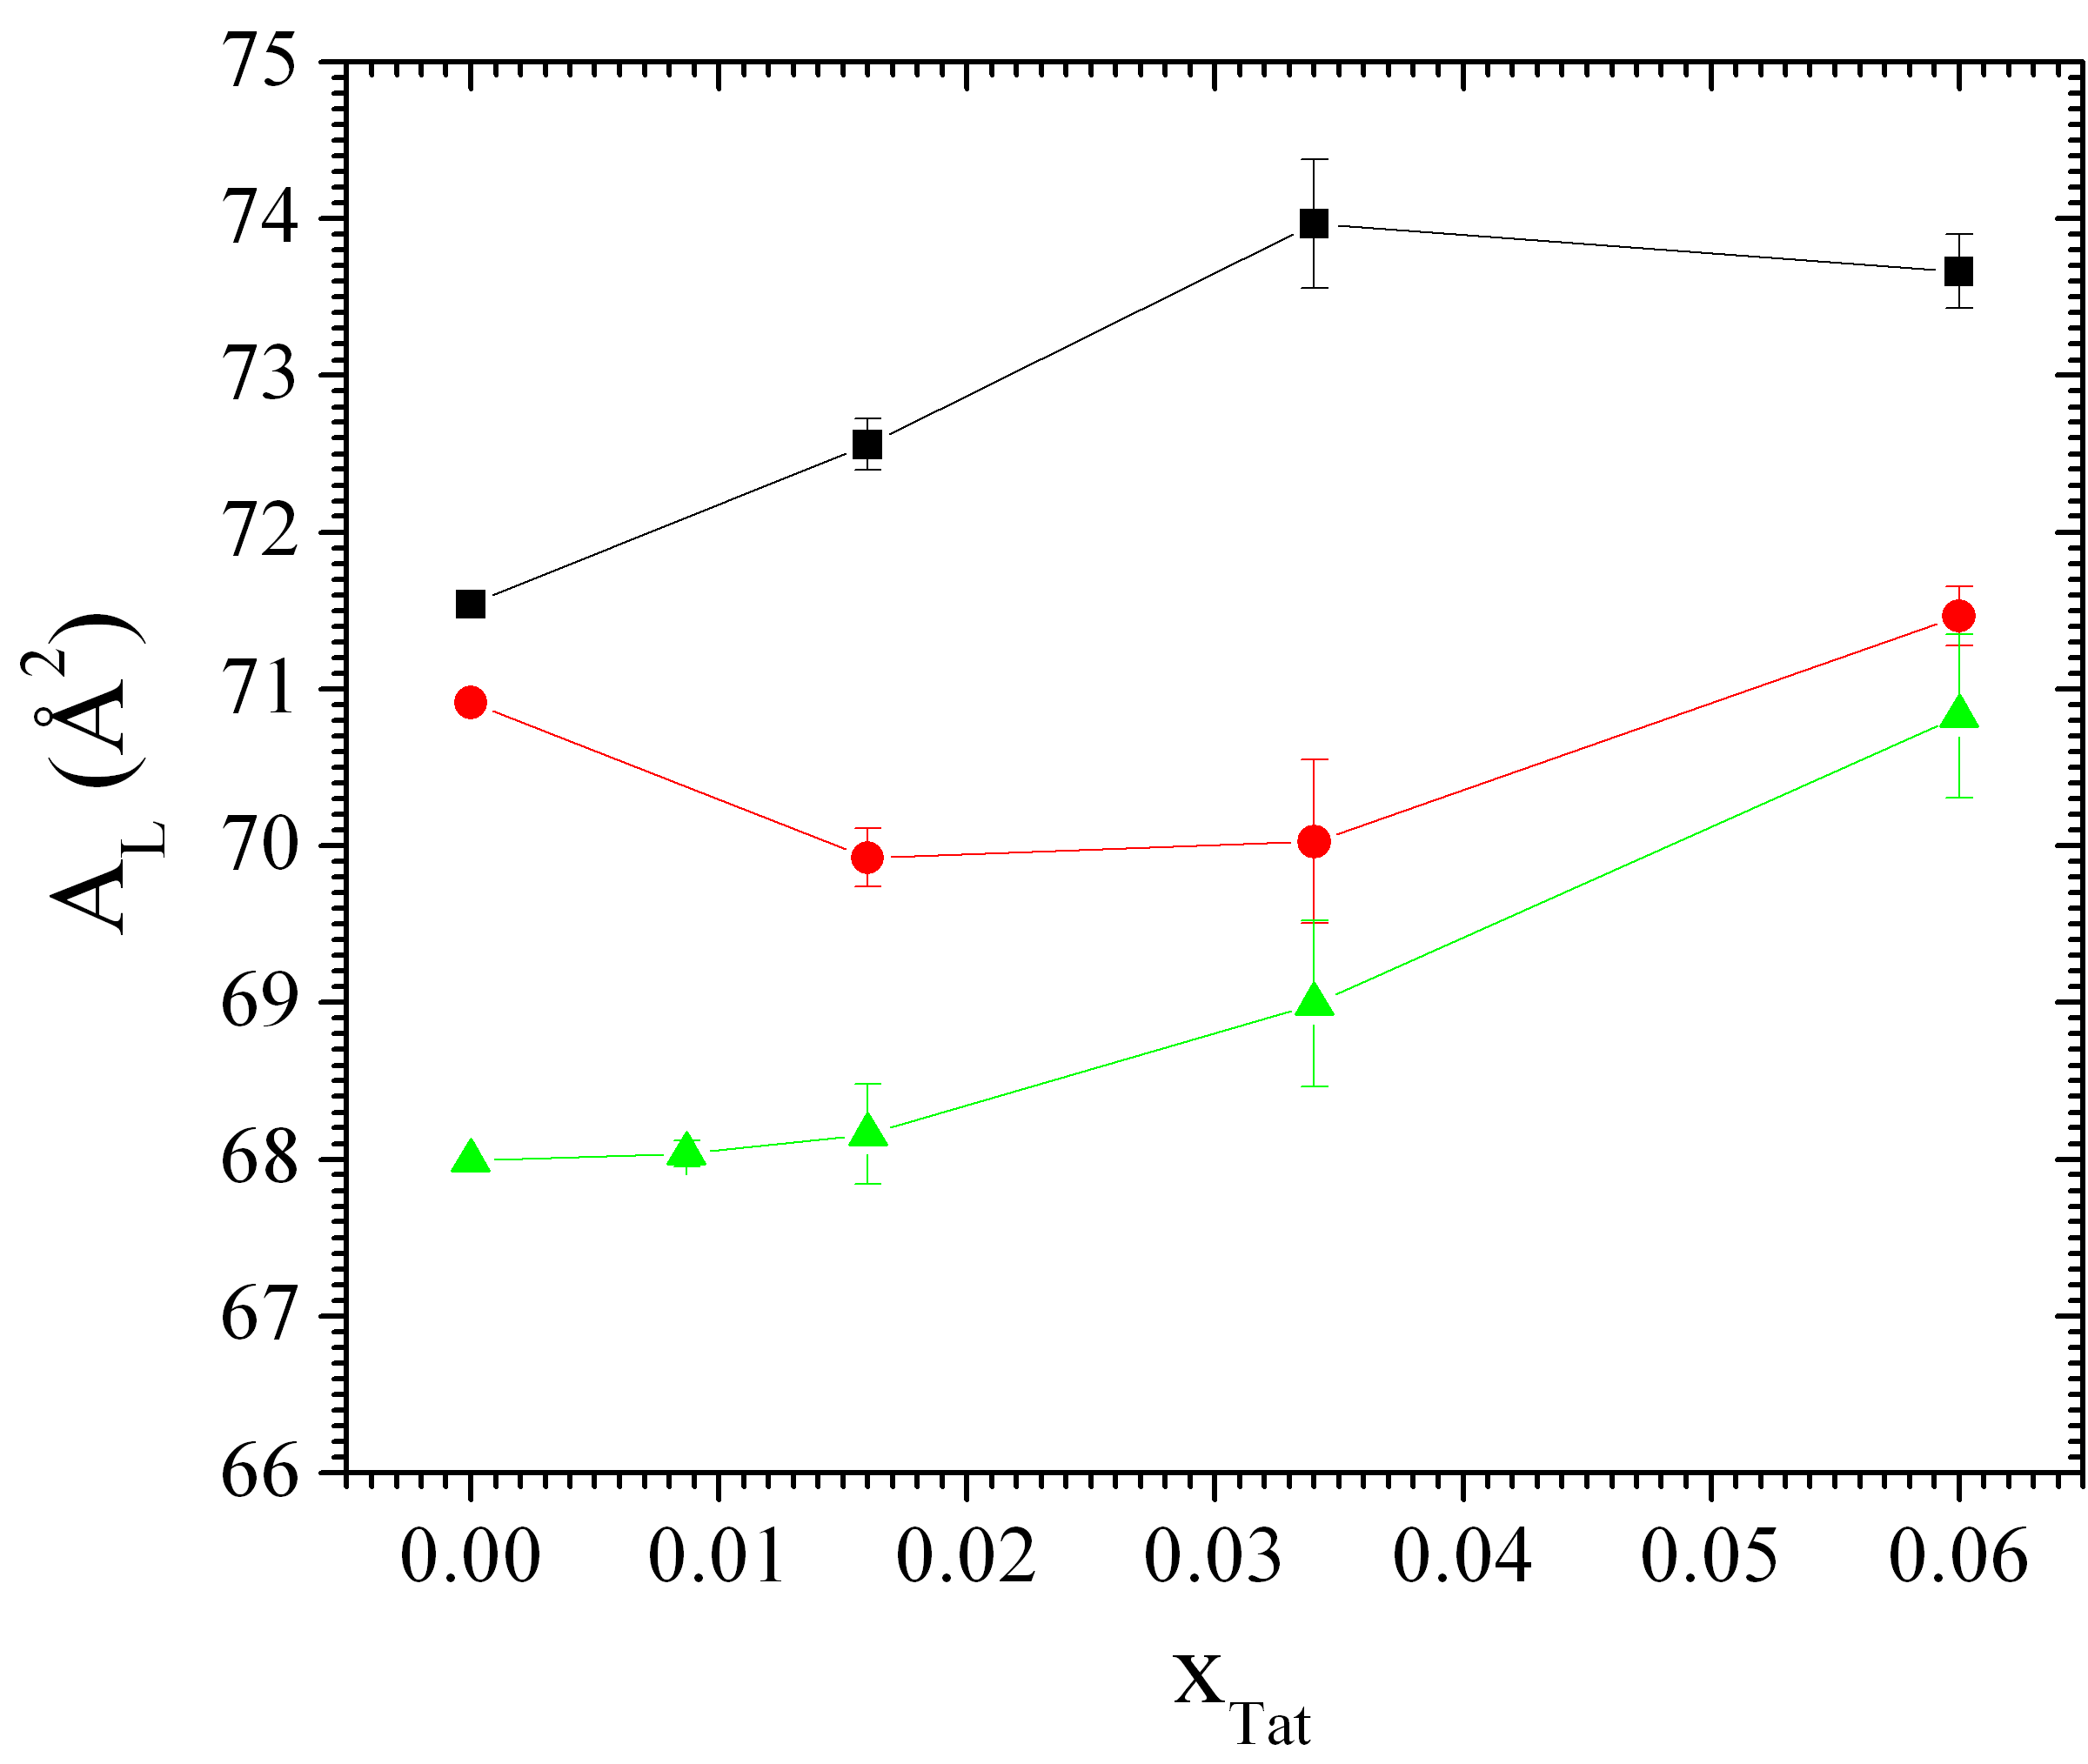
\includegraphics[width=0.49\textwidth]{figures/Tat/SDP_Results/AL}
  \caption[Area per lipid plotted against Tat mole fraction $\xTat$]
  {Area per lipid plotted against Tat mole fraction $\xTat$.
  Black squares (DOPC), red circles (DOPC:DOPE (3:1)), and green
  triangles (DOPC:DOPE (1:1)).
  Error bars are standard deviations from imposing Tat Gaussian widths, 
  $\sigmaTat$ = 2.5, 3.0 or 3.5 \AA.}
  \label{fig:AL}
\end{figure}

We also studied how the goodness of fit varied as the position of 
the Tat Gaussian was varied. Figure~\ref{fig:DOPC_Tat_X2} plots $\chi^2$ as a 
function of the fixed Tat position $\zTat$. We found that the two models,
THG (Tat-in-headgroup region) and THC (Tat-in-hydrocabon-chain region), resulted 
in similar electron density profiles, yielding similar $\chi^2$ values 
when Tat was placed near the hydrocarbon-water interface region. In the THC model, 
the error function representing the hydrocarbon chain region became wider as
Tat was placed closer to the interface region such that 
the total density profile calculated from the THC model was very similar to that calculated 
from the THG model.
In general, while the total electron density profile is well determined by 
our modeling procedures, the values of the parameters for the components are 
not as well determined as the agreement of the fit to the data may suggest. 
In many cases, we found multiple local minima in the fitting landscape, 
including one with Tat closer to the center of the bilayer as
shown in Fig.~\ref{fig:DOPC_Tat_X2}. $\chi^2$ calculated at these local minima 
tended to be smaller for larger concentration of Tat. We also found
that $\chi^2$ with $\zTat$ in the hydrocarbon chain region and headgroup
region was almost equal for the largest value of $\xTat$ for DOPC:DOPE (1:1)
bilayer.
The MD simulations performed by Dr. Kun Huang suggested that
the interior positions of Tat were artifacts of our model, at least for DOPC
bilayers. The simulation results are found in Sec.~\ref{sec:MD_results}.

%\begin{figure}[htbp]
%  \centering
%  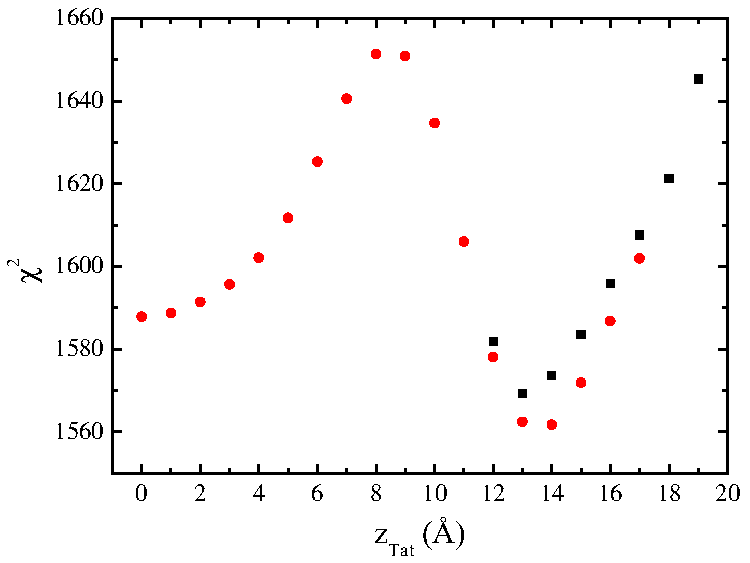
\includegraphics[width=0.3\textwidth]{figures/Tat/SDP_Results/X2/DOPC_Tat_62to1_3p0_X2}
%  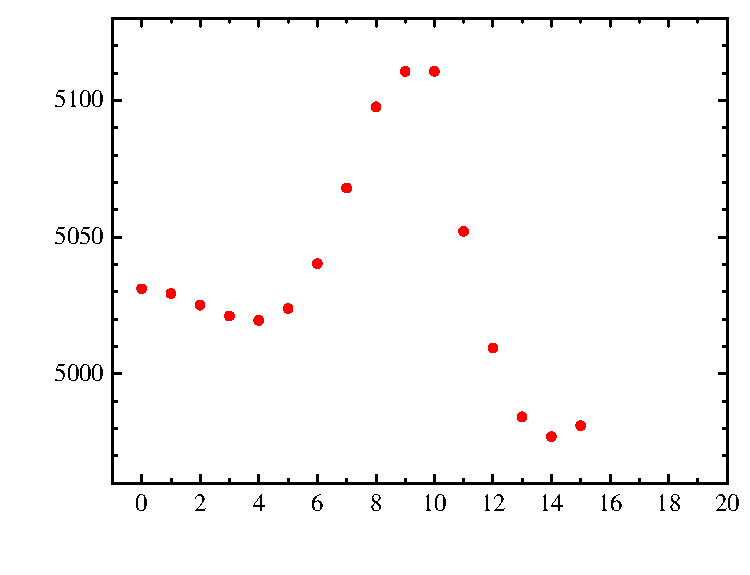
\includegraphics[width=0.3\textwidth]{figures/Tat/SDP_Results/X2/DOPCDOPE3to1_Tat_62to1_3p0_X2}
%  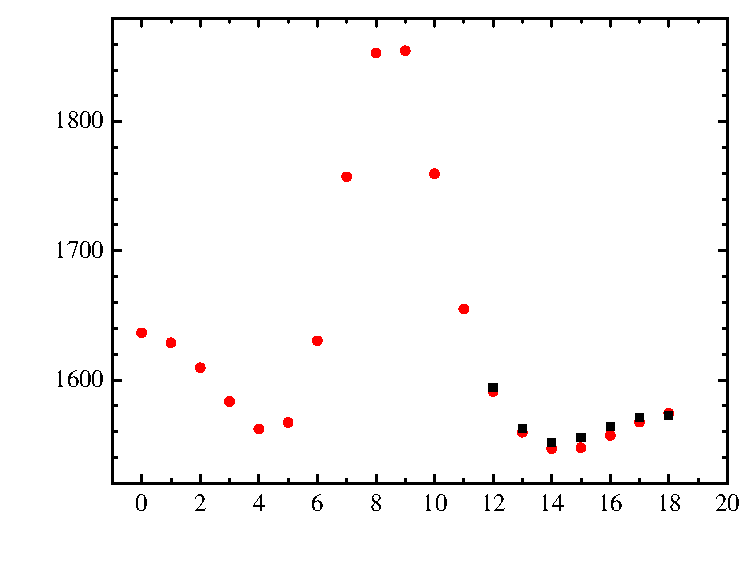
\includegraphics[width=0.3\textwidth]{figures/Tat/SDP_Results/X2/DOPCDOPE1to1_Tat_62to1_3p0_X2}
%  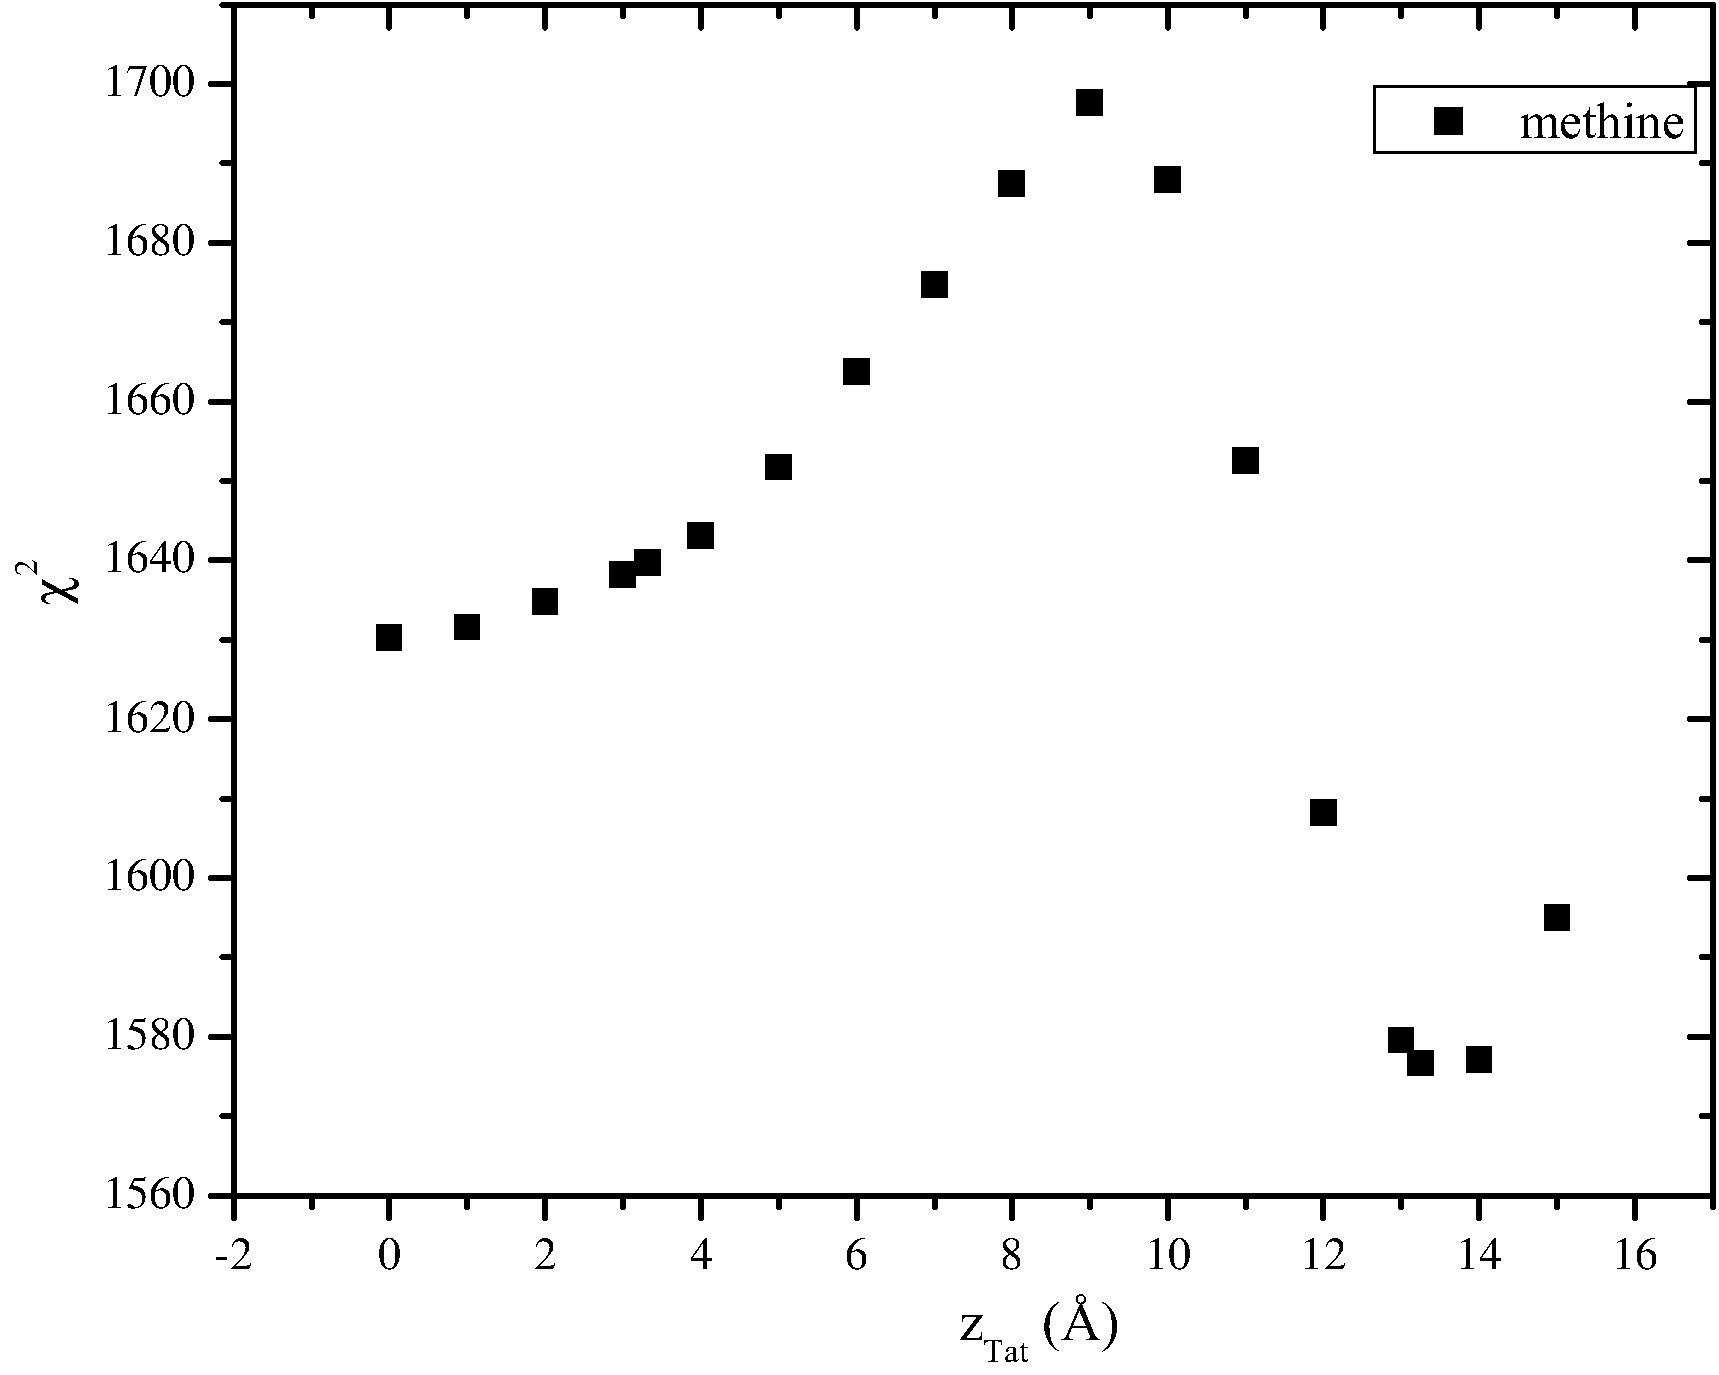
\includegraphics[width=0.3\textwidth]{figures/Tat/SDP_Results/X2/DOPC_Tat_28to1_3p0_X2}
%  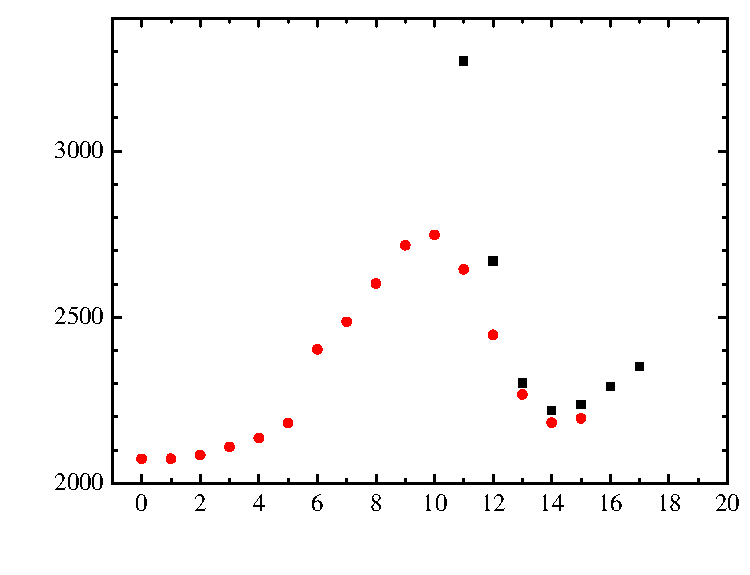
\includegraphics[width=0.3\textwidth]{figures/Tat/SDP_Results/X2/DOPCDOPE3to1_Tat_28to1_3p0_X2}
%  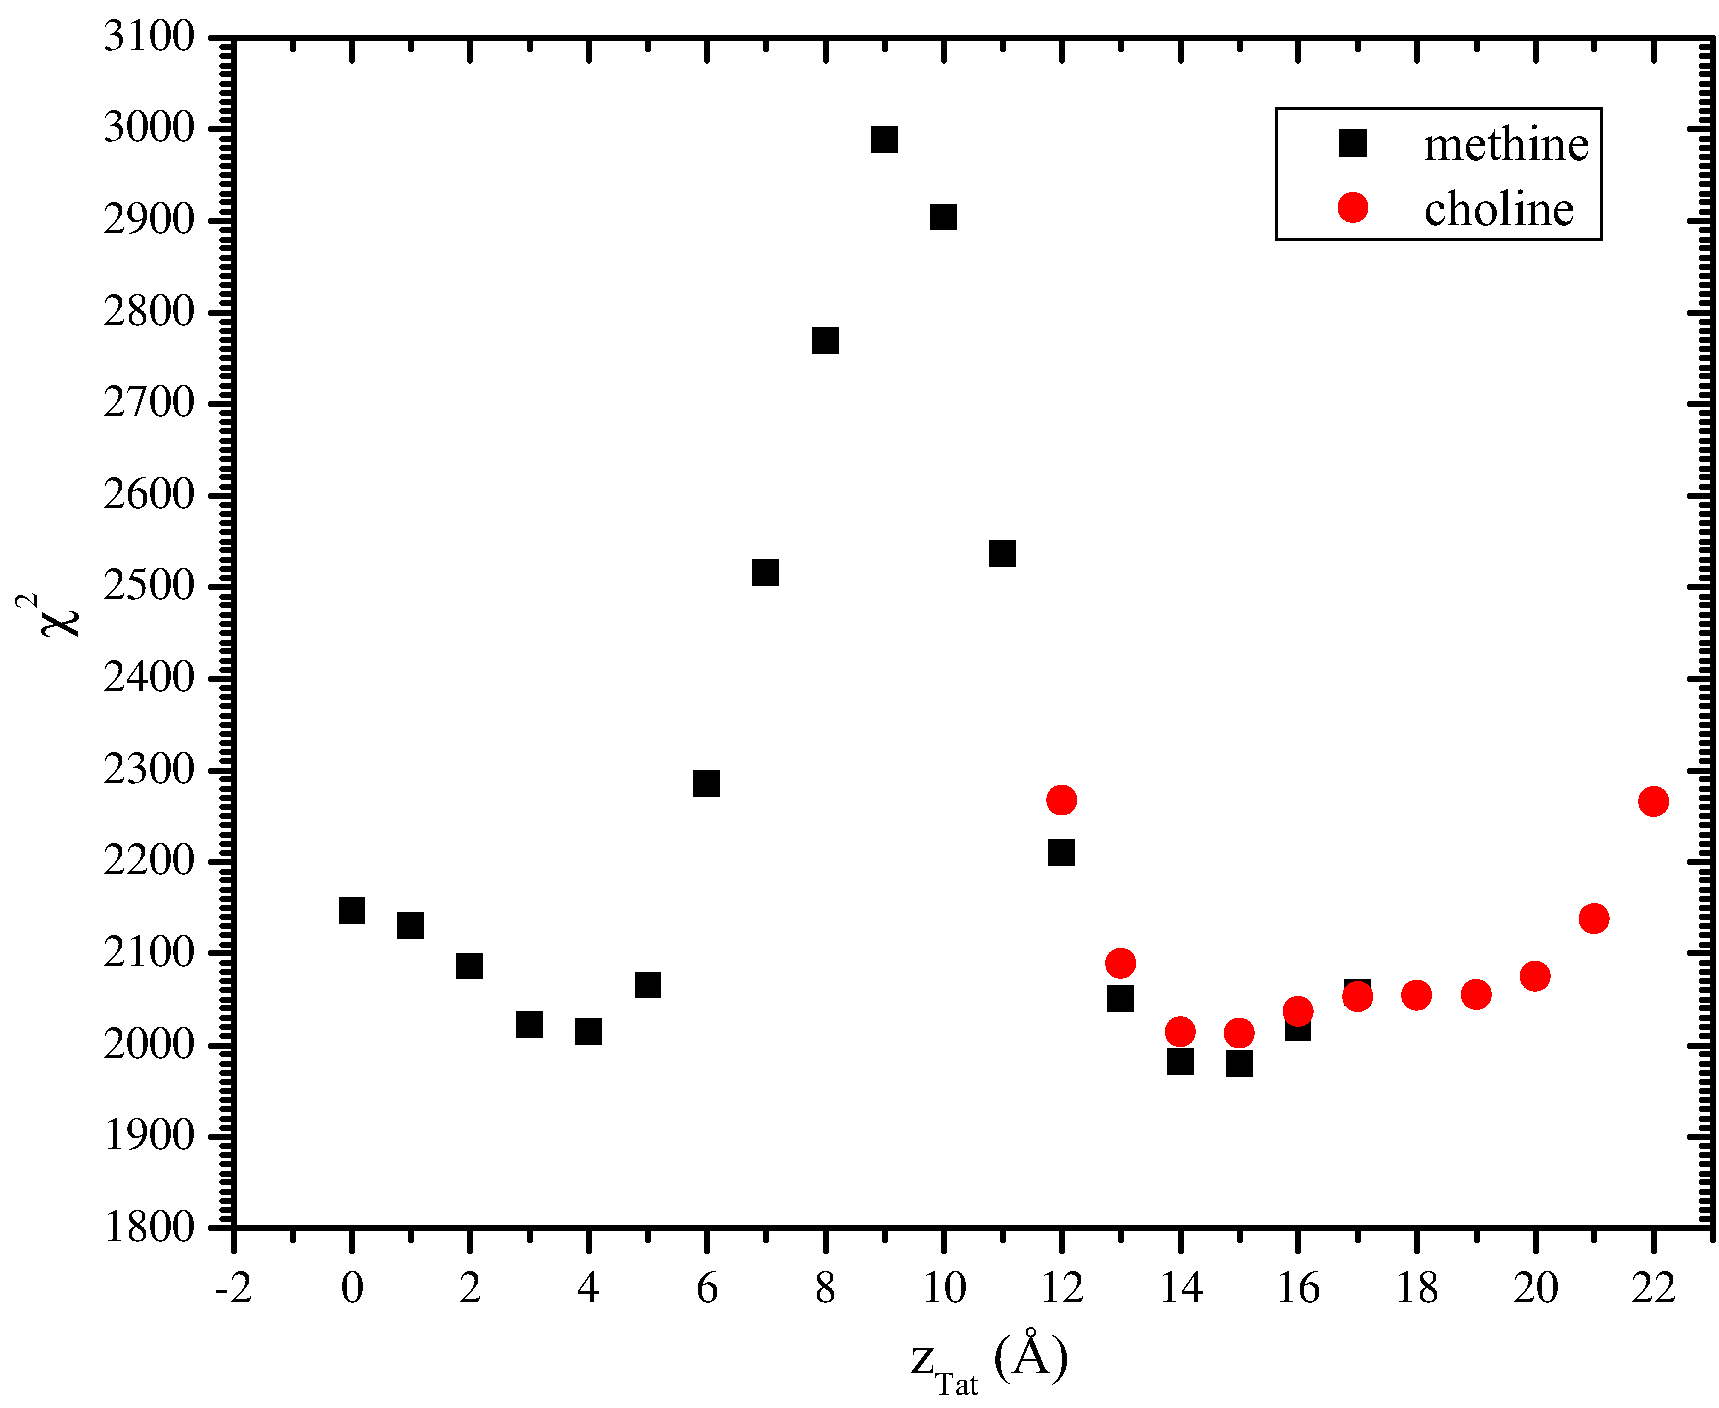
\includegraphics[width=0.3\textwidth]{figures/Tat/SDP_Results/X2/DOPCDOPE1to1_Tat_28to1_3p0_X2}
%  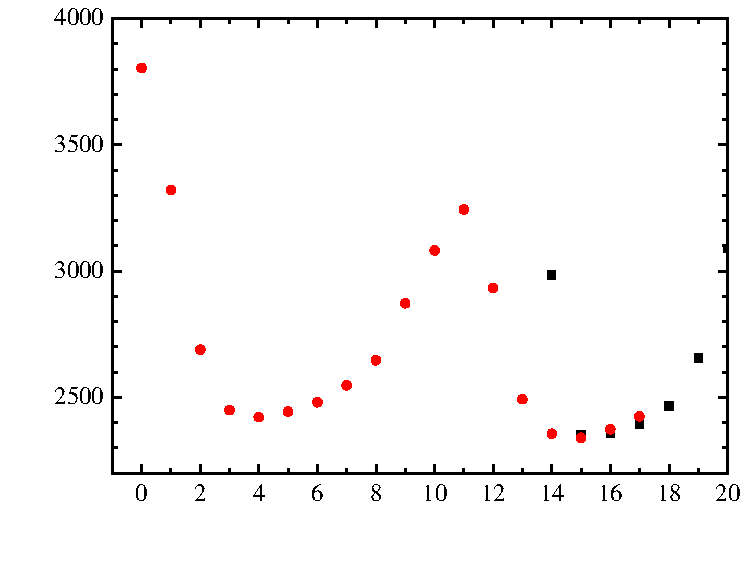
\includegraphics[width=0.3\textwidth]{figures/Tat/SDP_Results/X2/DOPC_Tat_16to1_3p0_X2}
%  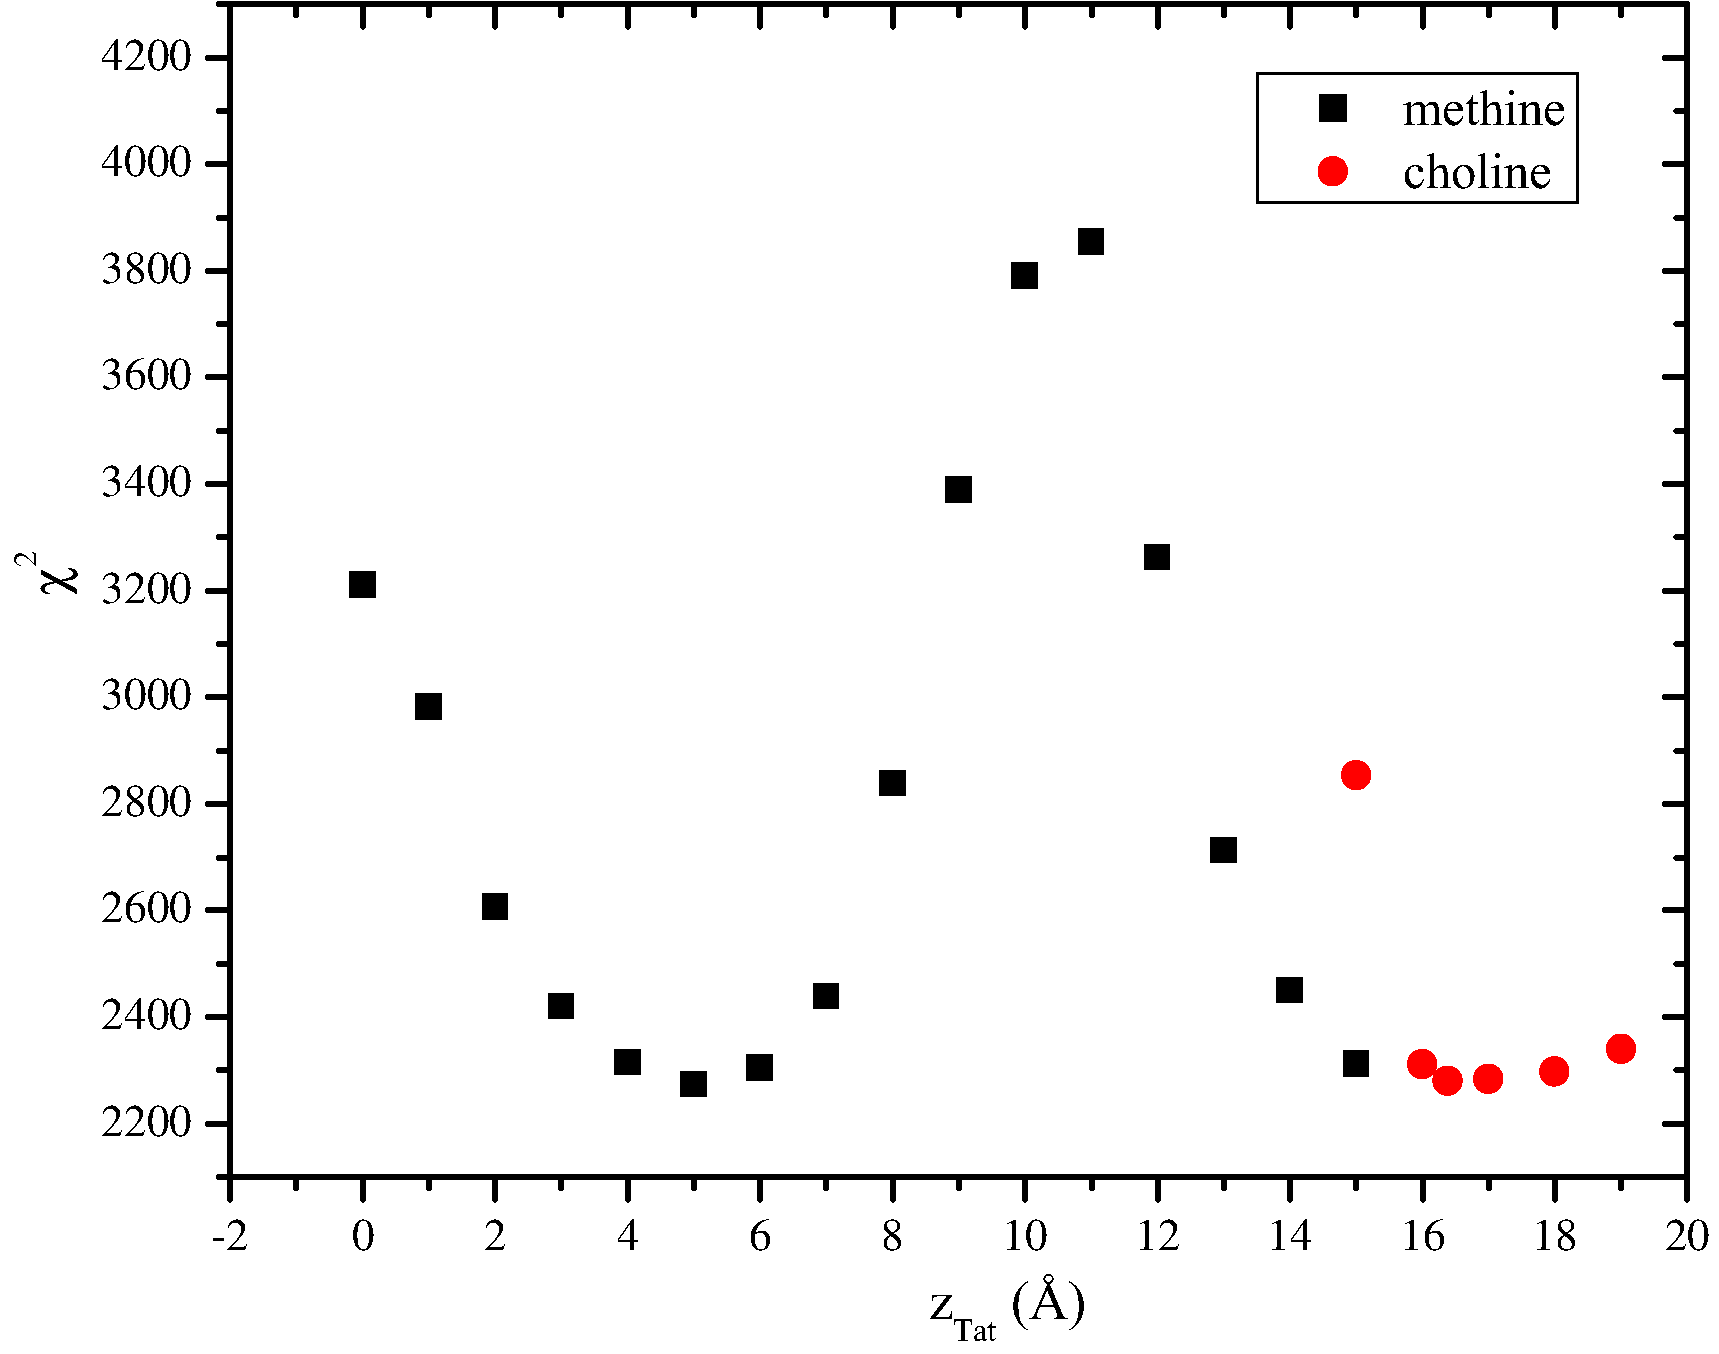
\includegraphics[width=0.3\textwidth]{figures/Tat/SDP_Results/X2/DOPCDOPE3to1_Tat_16to1_3p0_X2}
%  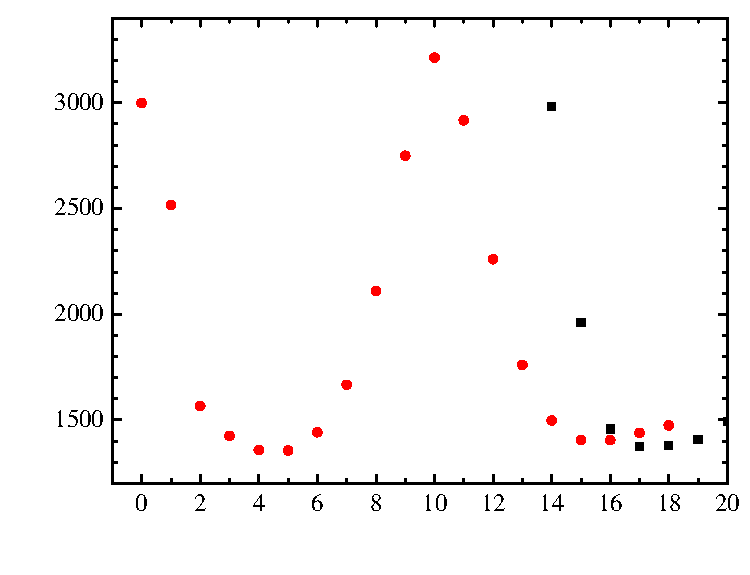
\includegraphics[width=0.3\textwidth]{figures/Tat/SDP_Results/X2/DOPCDOPE1to1_Tat_16to1_3p0_X2}
%  \caption{$\chi^2$ as a function of $\zTat$ for DOPC, DOPC:DOPE (3:1), and 
%  DOPC:DOPE (1:1) (from left to right) 
%  with $\xTat$ = 0.016, 0.034, and 0.059 (from top to bottom). 
%  $\sigmaTat = 3.0$. The THG model (black squares) and the THC model (red circles).}
%  \label{fig:DOPC_Tat_X2}
%\end{figure}

\begin{figure}[htbp]
  \centering
  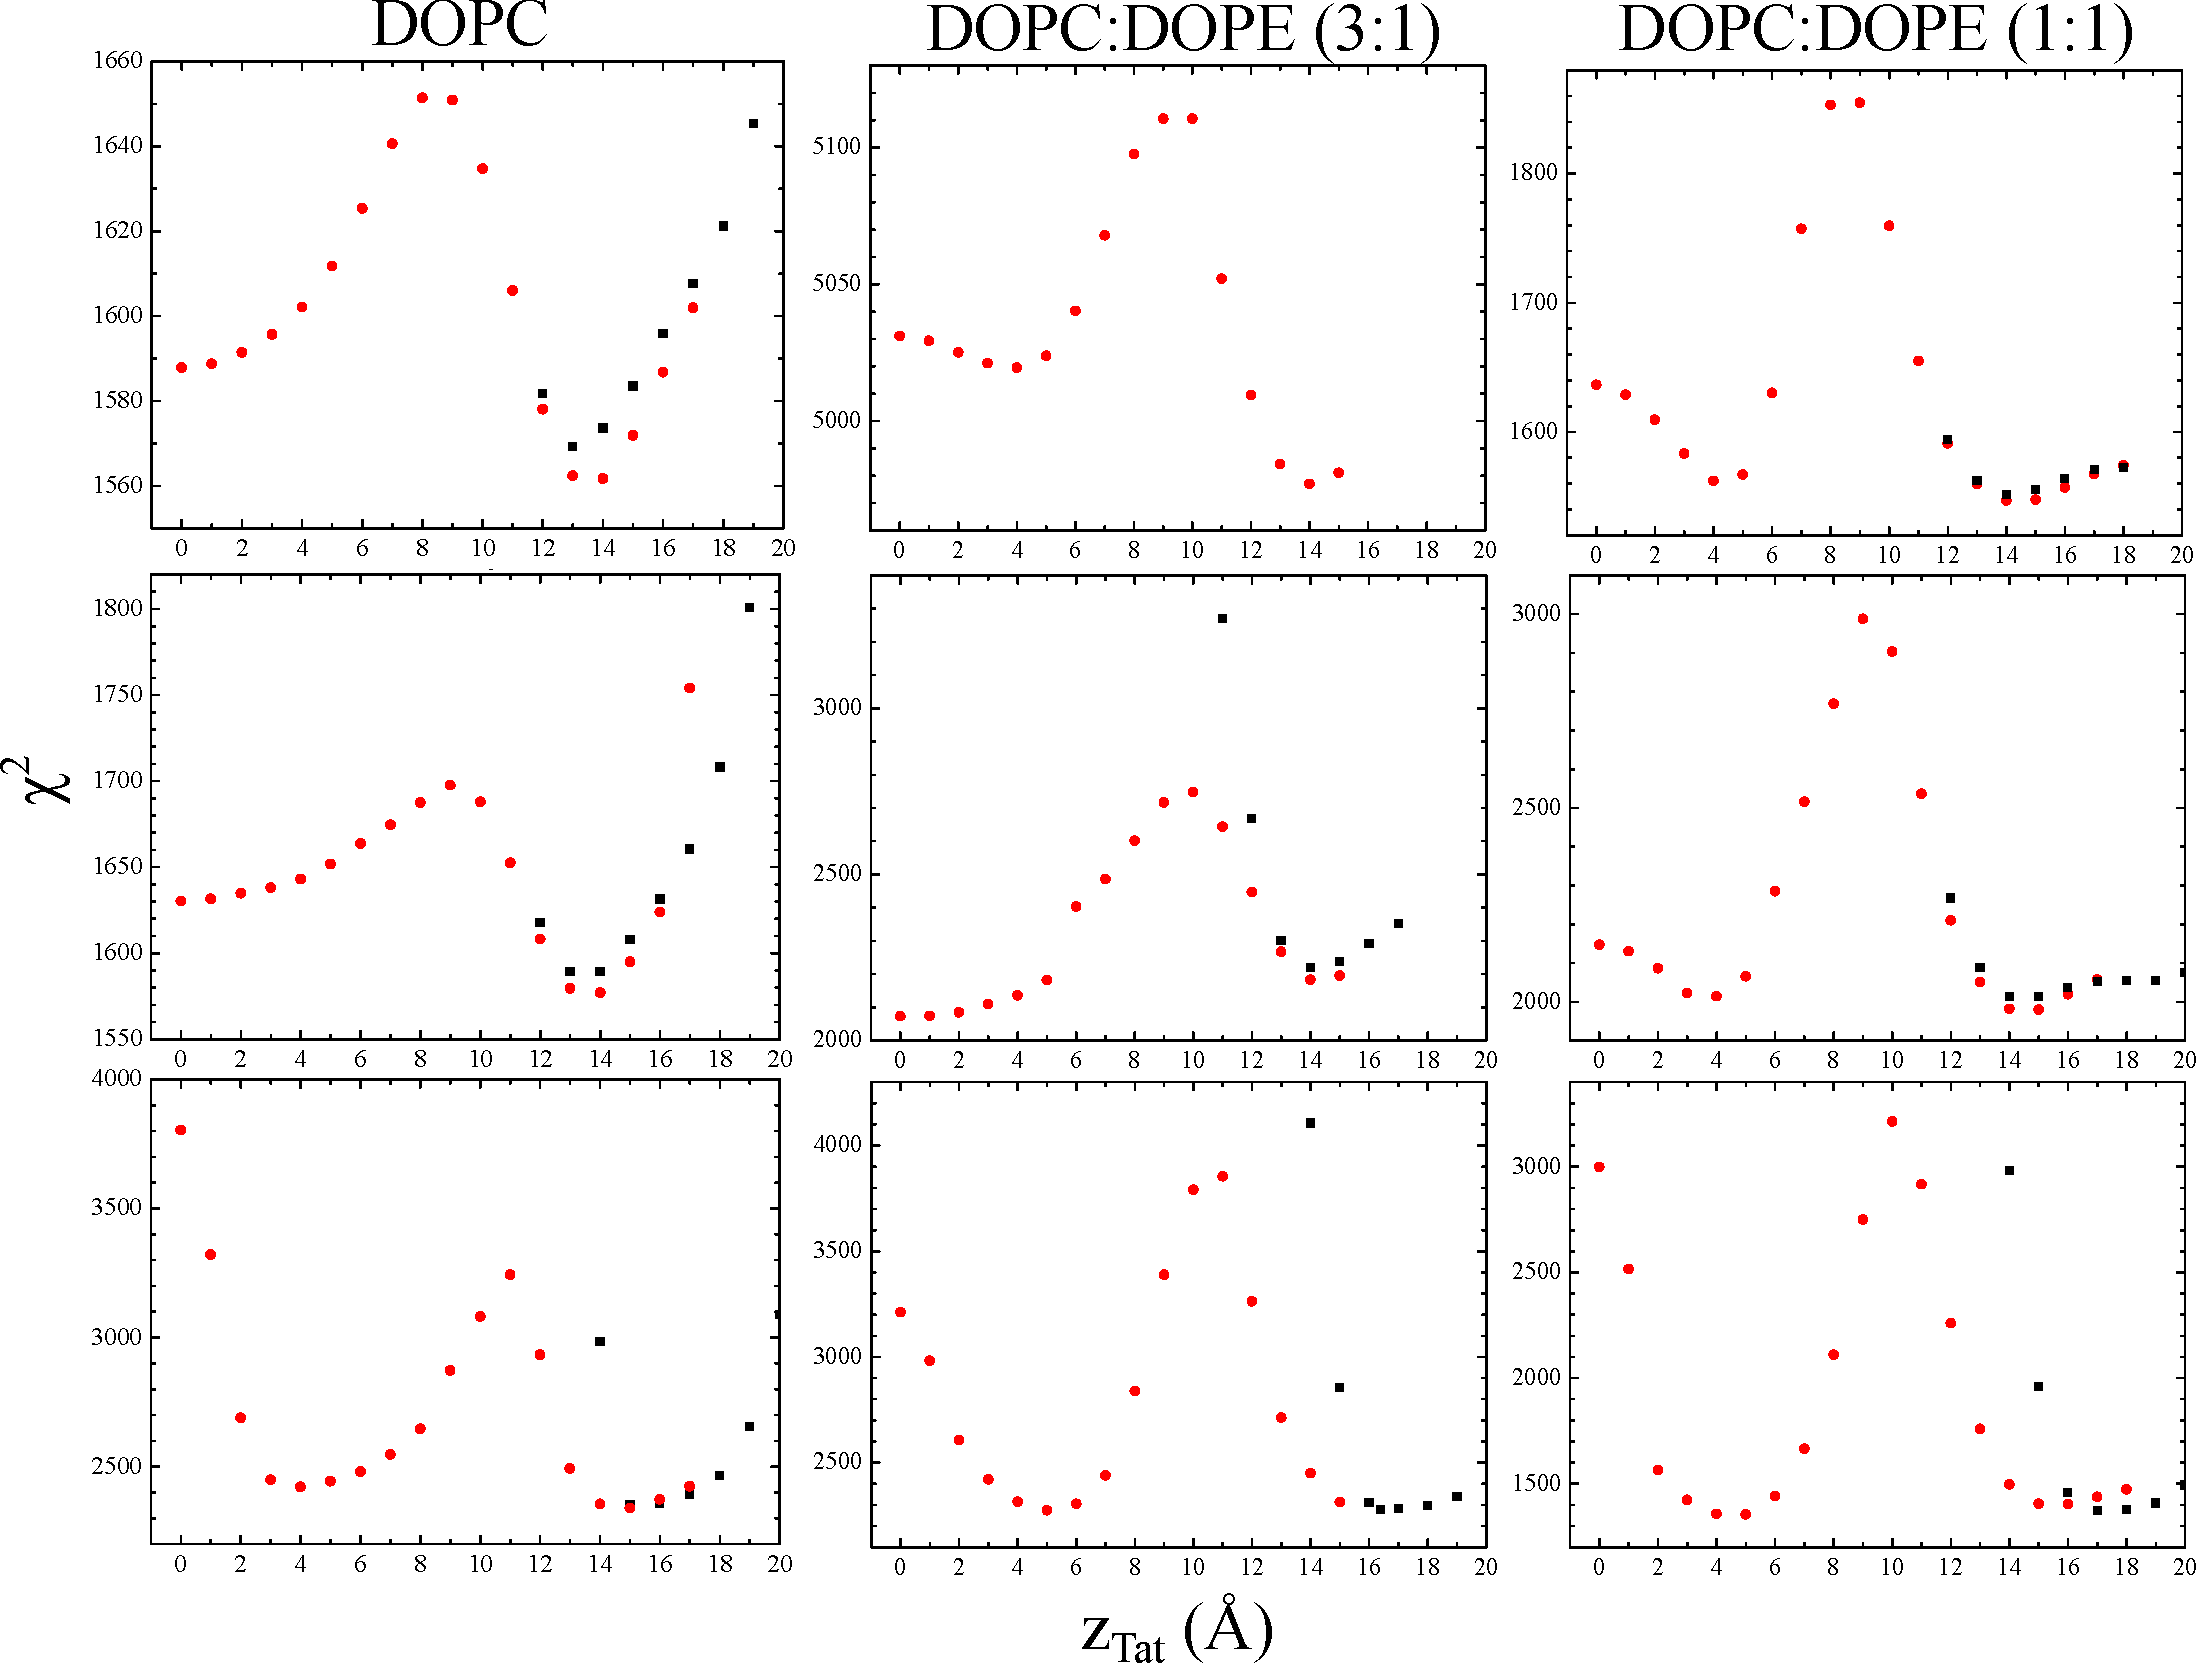
\includegraphics[width=\textwidth]{figures/Tat/SDP_Results/X2/X2}
  \caption[$\chi^2$ as a function of $\zTat$ for DOPC (left column), 
  DOPC:DOPE (3:1) (middle), and DOPC:DOPE (1:1) (right) 
  with $\xTat$ = 0.016 (top row), 0.034 (middle), and 0.059 (bottom)]
  {$\chi^2$ as a function of $\zTat$ for DOPC (left column), 
  DOPC:DOPE (3:1) (middle), and DOPC:DOPE (1:1) (right) 
  with $\xTat$ = 0.016 (top row), 0.034 (middle), and 0.059 (bottom). 
  $\sigmaTat = 3.0$. The THG model (black squares) and the THC model (red circles).}
  \label{fig:DOPC_Tat_X2}
\end{figure}

As seen from Table~\ref{tab:DOPC_fit_results}, 
the widths of the headgroup components
became smaller as Tat concentration increased. This
decrease seemed somewhat unreasonable; if Tat causes a bilayer 
to locally become thinner, 
we would expect the headgroup components to become
wider. Therefore, we also fitted a model with lower bounds
on these headgroup widths. Namely, the minimum values of the widths of
the headgroup components, PC and CG, were constrained to be greater than
or equal to the corresponding values for pure bilayers without Tat. 
Table~\ref{tab:bound_DOPC} shows results from fitting the data with
lower bounds on the widths of the headgroup components for DOPC/Tat systems.
In all cases, both headgroup widths, $\sigmaPC$ and $\sigmaCG$, resulted 
in the same value as the value of their corresponding lower bounds. 
Similarly to fits with unbound widths, $\DPP=2\zPC$ decreased as Tat concentration
increased. The biggest difference between these bound fits and the unbound fits
is in Tat position $\zTat$. Figure~\ref{fig:zTat_bound} plots $\zTat$ as a function
of Tat mole fraction $\xTat$ for both fits with and without lower bounds.
While $\zTat$ increased as $\xTat$ increased for fits without bounds, $\zTat$
stayed more or less constant for fits with the bounds. Moreover, 
Table~\ref{tab:bound_DOPC} shows that 
Tat was located closer to the PC headgroup than the CG headgroup
for fits with the lower bounds. Thus,
depth of Tat insertion was influenced strongly by the lipid headgroup widths.
In order to gain better understanding of location of Tat in DOPC bilayers,
we now turn to MD simulations.

\begin{table}[htbp]
  \centering
  \begin{tabular}{c|c|ccc|ccc|ccc}
  \hline 
    $\xTat$ & 0  &    0.016 & 0.016 & 0.016 & 0.034 & 0.034 & 0.034 & 0.059 & 0.059 & 0.059 \\
    \hline
    $\chi^2$ & 2961 & {\color{red}1853} & 1979 & 2118 & {\color{red}2398} & 2893 & 3414    & {\color{red}3160} & 4298 & 5539 \\   
    $\zPC$ & 18.1   &    17.8 & 17.8 & 17.8 & 17.4 & 17.4 & 17.4    & 17.5 & 17.4 & 17.3 \\   
    $\sigmaPC$  & 2.5 &   2.5* &  2.5* &  2.5* & 2.5* & 2.5* & 2.5*       & 2.5* & 2.5* & 2.5* \\      
    $\zCG$   & 15.0 &    14.7 & 14.7 & 14.7 & 14.3 & 14.3 & 14.3    & 14.4 & 14.4 & 14.3 \\   
    $\sigmaCG$ & 3.0 &    3.0* &  3.0* &  3.0* & 3.0* & 3.0* & 3.0* & 3.0* & 3.0* & 3.0* \\      
    $\zHC$ & 13.7 &     13.4 & 13.4 & 13.4  & 13.0 & 13.0 & 13.0    & 13.1 & 13.0 & 12.9 \\   
    $\sigmaHC$ &      3.0 &2.7 & 2.7 & 2.7  & 2.7 & 2.7 & 2.7       & 2.7 & 2.7 & 2.7 \\      
    $\sigmaCHthree$ & 3.2 & 3.1 & 3.1 & 3.1 & 3.6 & 3.6 & 3.7       & 2.6 & 2.6 & 2.5 \\      
    $\zTat$ & -- &          16.9 & 16.8 & 17.0 & 16.4 & 16.5 & 16.7    & 16.3 & 16.6 & 17.1 \\   
    $\sigmaTat$ & -- &         2.5 & 3.0 & 3.5 & 2.5 & 3.0 & 3.5       & 2.5 & 3.0 & 3.5 \\      
    $\AL$ & 71.5 &       73.5 & 73.5 & 73.5 & 75.6 & 75.6 & 75.6    & 75.0 & 75.4 & 75.9 \\    
  \hline
  \end{tabular}
  \caption[Fitting Results for the THG model with the lower bounds on the headgroup
  widths for DOPC membranes]
  {Fitting Results for the THG model with the lower bounds on the headgroup
  widths for DOPC membranes. 
  The smallest $\chi^2$ values at each Tat mole fraction $\xTat$ are highlighted in red. 
  $\zPC-\zCG$ = 3.1 and $\zCG-\zHC$ = 1.3 in all fits. 
  Units of all symbols are \AA\ except for $\chi^2$ (unitless) and $\AL$ (\AA$^2$).  
  \\
  *Parameters with a lower bound as described in the text}
  \label{tab:bound_DOPC}
\end{table}

\begin{figure}[htbp]
  \centering
  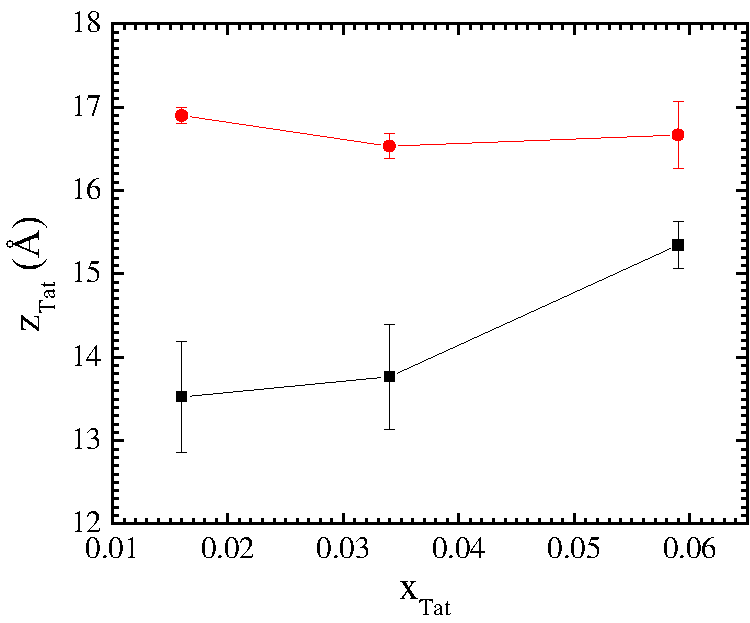
\includegraphics[width=0.45\textwidth]{figures/Tat/SDP_Results/zTat_bound}
  \caption[$\zTat$ as a function of Tat mole fraction $\xTat$ for fits with
  lower bounds on the headgroup widths (red circles) and without lower 
  bounds (black squares)]
  {$\zTat$ as a function of Tat mole fraction $\xTat$ for fits with
  lower bounds on the headgroup widths (red circles) and without lower 
  bounds (black squares). 
  Error bars are standard deviations from imposing Tat Gaussian widths, 
  $\sigmaTat$ = 2.5, 3.0 or 3.5 \AA.}
  \label{fig:zTat_bound}
\end{figure}

\begin{figure}[htbp]
  \centering
  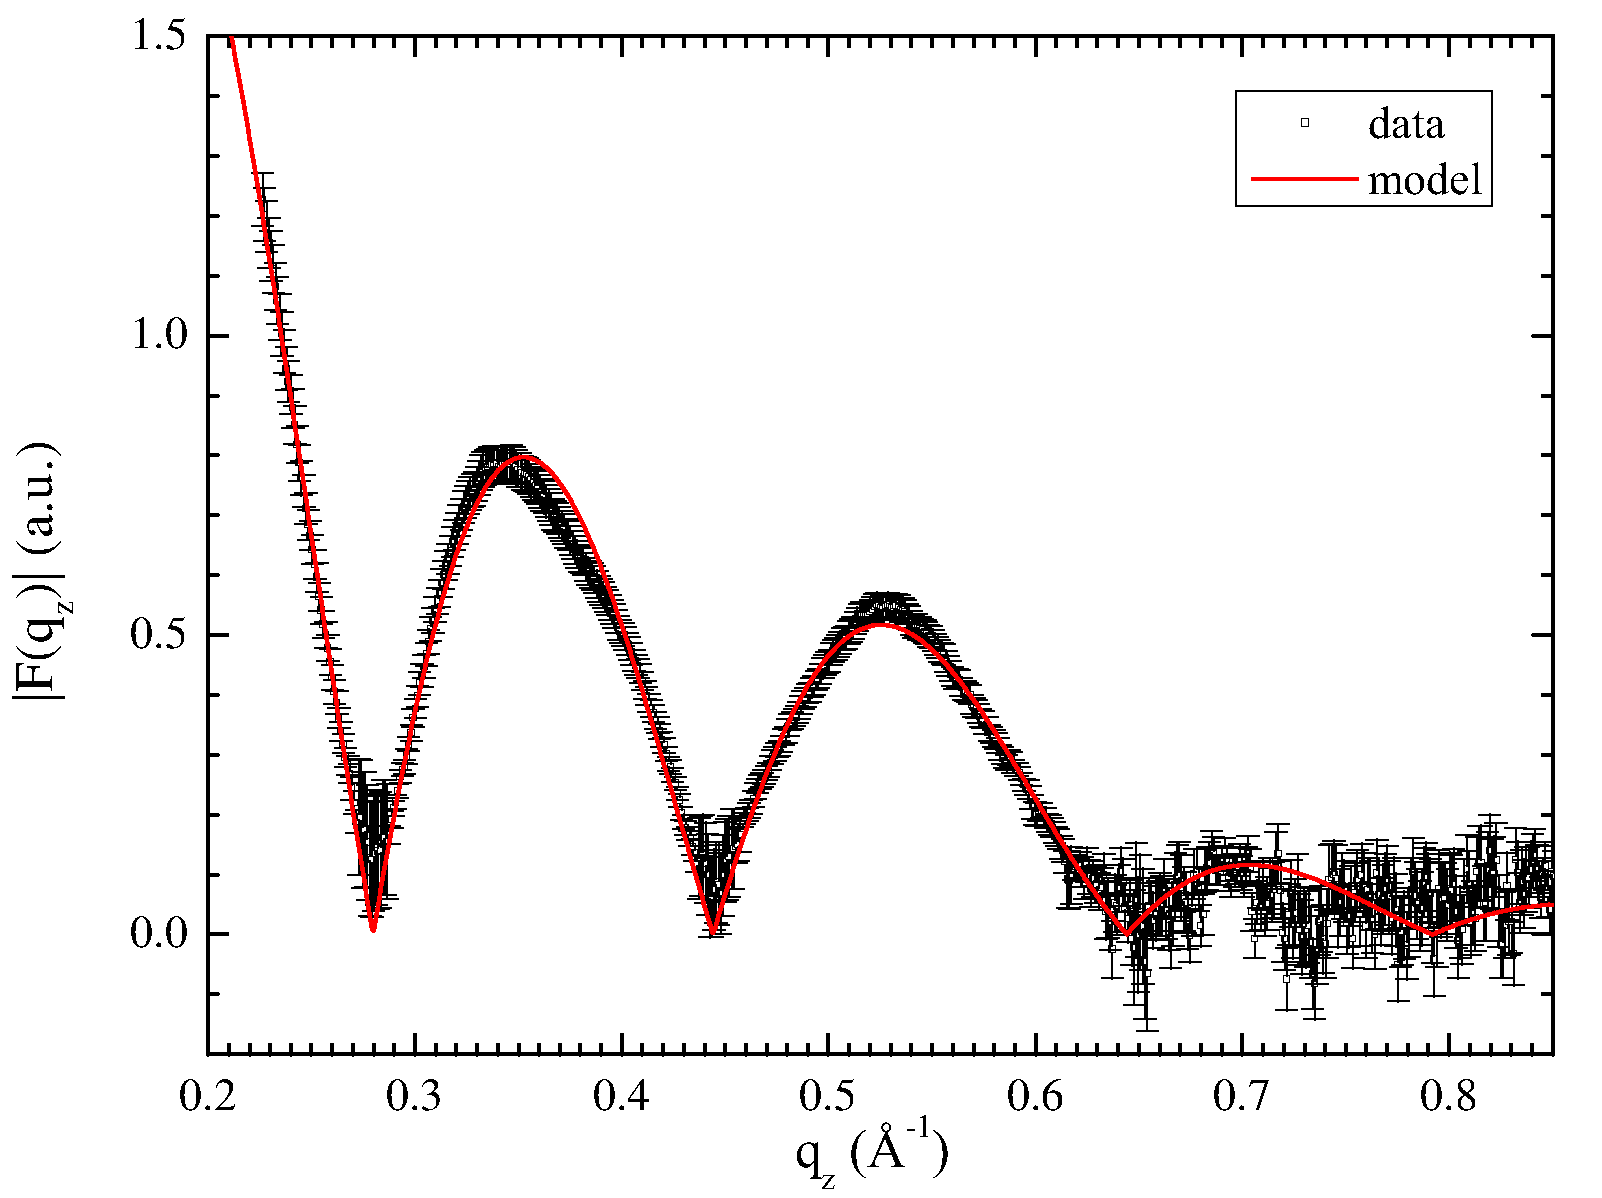
\includegraphics[trim=5 30 0 0,clip=true,width=0.47\textwidth]{figures/Tat/SDP_Results/XFF/DOPCDOPE3to1_XFF1}
  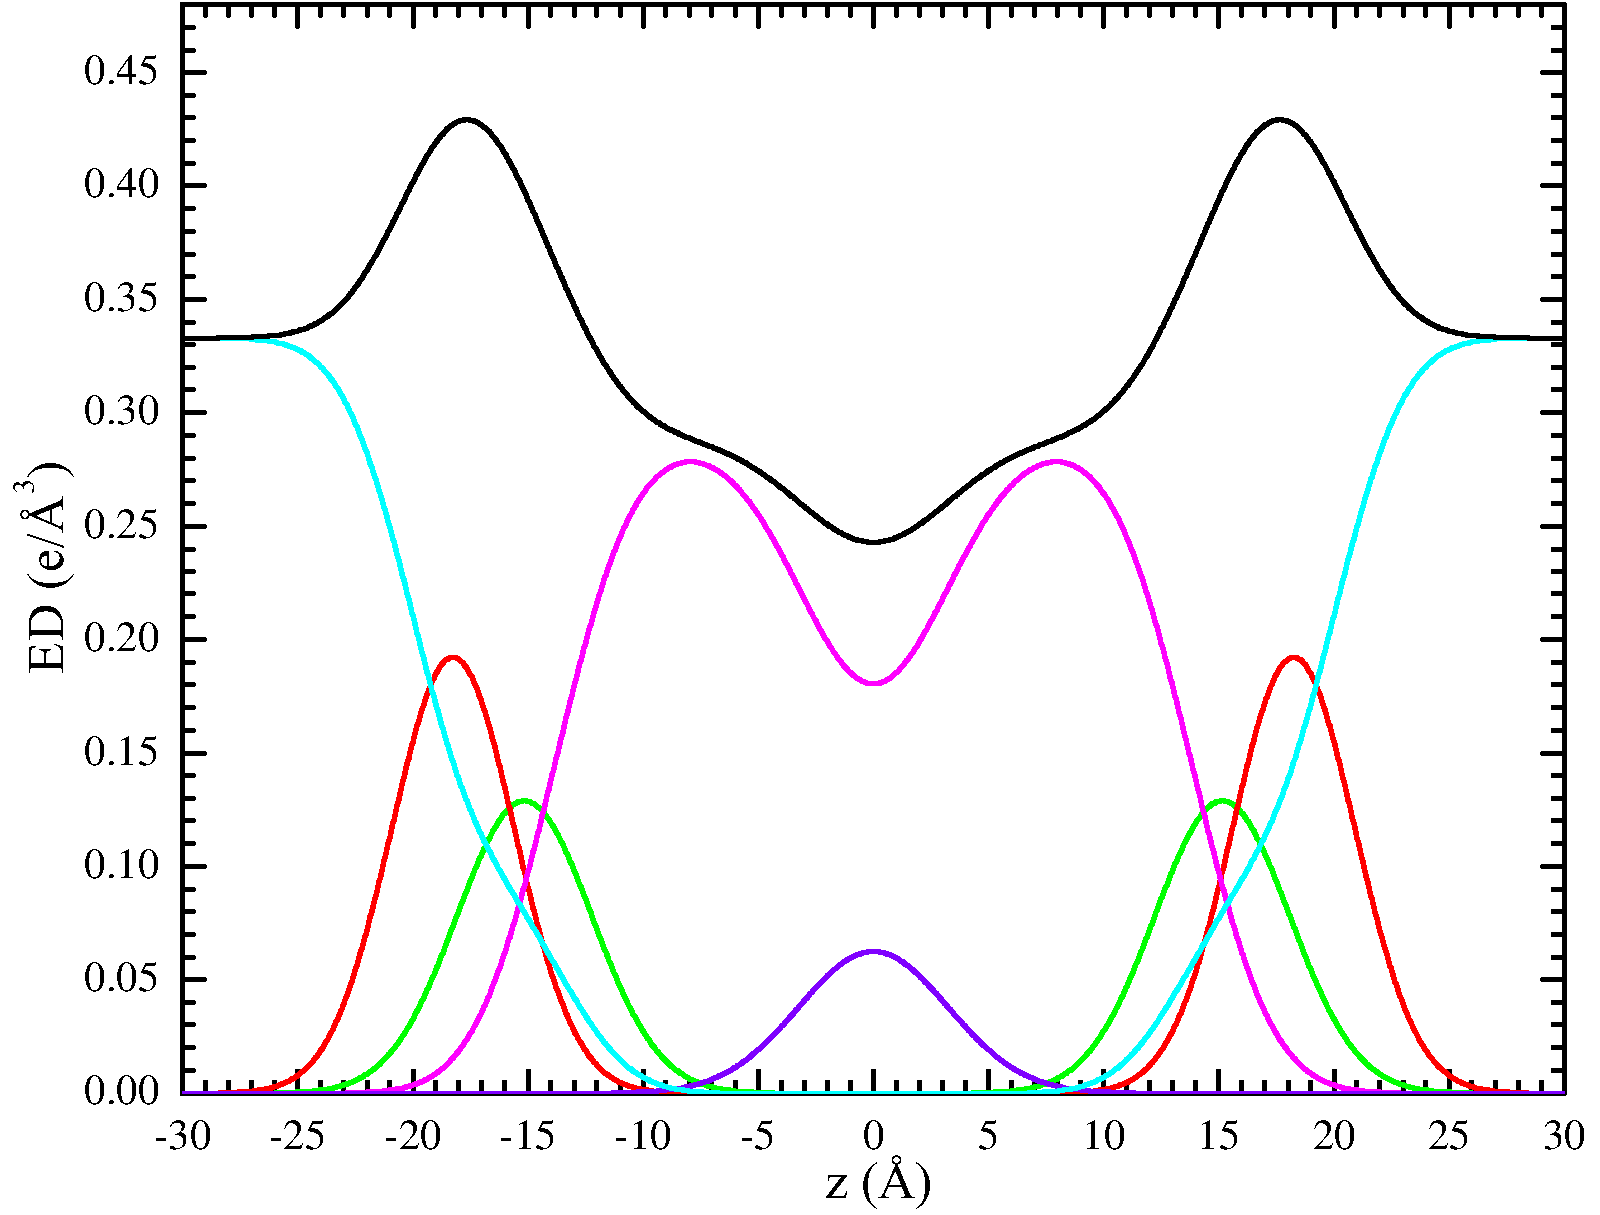
\includegraphics[trim=5 30 0 0,clip=true,width=0.47\textwidth]{figures/Tat/SDP_Results/EDP/DOPCDOPE3to1_EDP1}
  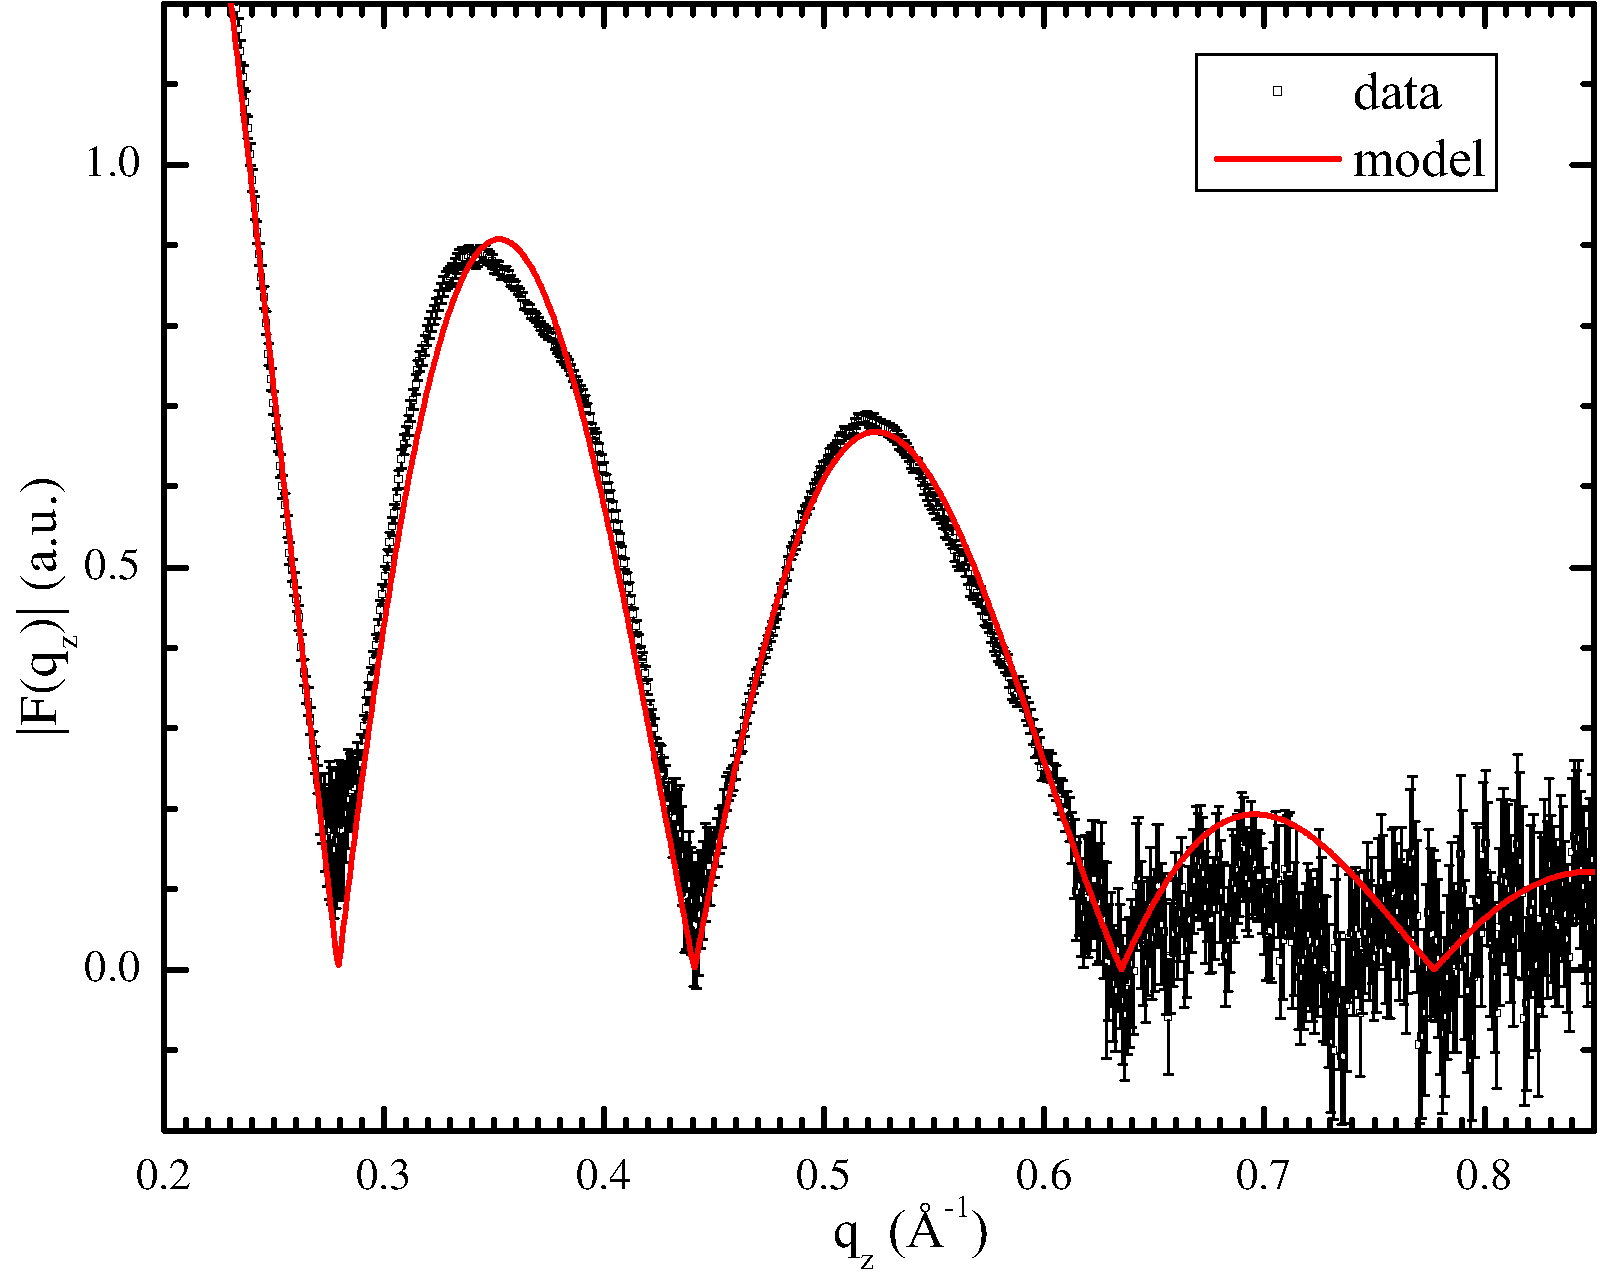
\includegraphics[trim=5 30 0 0,clip=true,width=0.47\textwidth]{figures/Tat/SDP_Results/XFF/DOPCDOPE3to1_Tat_62to1_3p0_XFF1}
  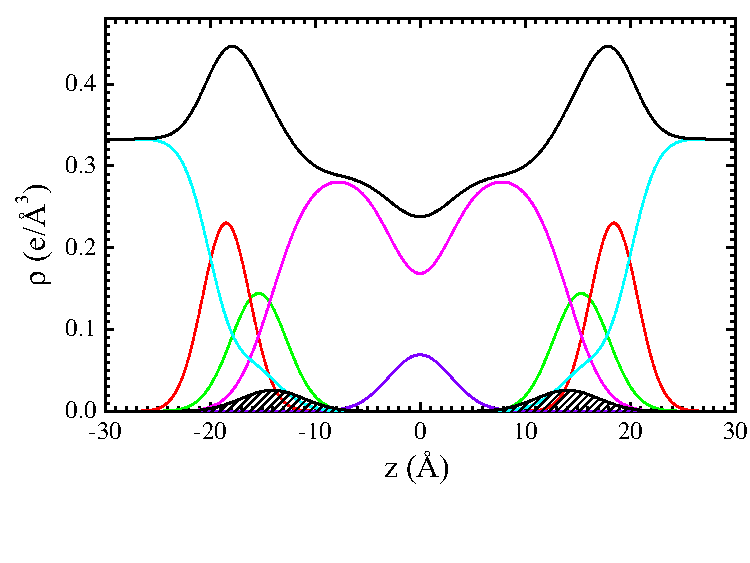
\includegraphics[trim=5 30 0 0,clip=true,width=0.47\textwidth]{figures/Tat/SDP_Results/EDP/DOPCDOPE3to1_Tat_62to1_3p0_EDP1}
  \includegraphics[trim=5 30 0 0,clip=true,width=0.47\textwidth]{figures/Tat/SDP_Results/XFF/DOPCDOPE3to1_Tat_28to1_3p0_XFF1}
  \includegraphics[trim=5 30 0 0,clip=true,width=0.47\textwidth]{figures/Tat/SDP_Results/EDP/DOPCDOPE3to1_Tat_28to1_3p0_EDP1}
  \includegraphics[trim=5 30 0 0,clip=true,width=0.47\textwidth]{figures/Tat/SDP_Results/XFF/DOPCDOPE3to1_Tat_16to1_3p0_XFF1}
  \includegraphics[trim=5 30 0 0,clip=true,width=0.47\textwidth]{figures/Tat/SDP_Results/EDP/DOPCDOPE3to1_Tat_16to1_3p0_EDP1} 
  %\includegraphics[width=0.45\textwidth,valign=t]{./figures/Tat/SDP_Results/EDP/DOPCDOPE3to1_Tat_16to1_3p0_EDP1}
  \caption[Best fits to DOPC:DOPE (3:1) form factors (left) and the corresponding 
  electron density profiles (right) with $\xTat$ = 0, 0.016, 0.034, 
  and 0.059 (from top to bottom)]
  {Best fits to DOPC:DOPE (3:1) form factors (left) and the corresponding 
  electron density profiles (right) with $\xTat$ = 0, 0.016, 0.034, 
  and 0.059 (from top to bottom).
  The Tat EDP is a solid black line with diagonal line underfill.}
  \label{fig:DOPCDOPE3to1_Tat_XFF1}
\end{figure}

\begin{figure}[htbp]
  \centering
  \includegraphics[trim=5 30 0 0,clip=true,width=0.47\textwidth]{figures/Tat/SDP_Results/XFF/DOPCDOPE1to1_XFF1}
  \includegraphics[trim=5 30 0 0,clip=true,width=0.47\textwidth]{figures/Tat/SDP_Results/EDP/DOPCDOPE1to1_EDP1}
  \includegraphics[trim=5 30 0 0,clip=true,width=0.47\textwidth]{figures/Tat/SDP_Results/XFF/DOPCDOPE1to1_Tat_62to1_3p0_XFF1}
  \includegraphics[trim=5 30 0 0,clip=true,width=0.47\textwidth]{figures/Tat/SDP_Results/EDP/DOPCDOPE1to1_Tat_62to1_3p0_EDP1}
  \includegraphics[trim=5 30 0 0,clip=true,width=0.47\textwidth]{figures/Tat/SDP_Results/XFF/DOPCDOPE1to1_Tat_28to1_3p0_XFF1}
  \includegraphics[trim=5 30 0 0,clip=true,width=0.47\textwidth]{figures/Tat/SDP_Results/EDP/DOPCDOPE1to1_Tat_28to1_3p0_EDP1}
  \includegraphics[trim=5 30 0 0,clip=true,width=0.47\textwidth]{figures/Tat/SDP_Results/XFF/DOPCDOPE1to1_Tat_16to1_3p0_XFF1}
  \includegraphics[trim=5 30 0 0,clip=true,width=0.47\textwidth]{figures/Tat/SDP_Results/EDP/DOPCDOPE1to1_Tat_16to1_3p0_EDP1}
  \caption[Best fits to DOPC:DOPE (1:1) form factors (left) and the corresponding 
  electron density profiles (right) with $\xTat$ = 0, 0.016, 0.034, 
  and 0.059 (from top to bottom)]
  {Best fits to DOPC:DOPE (1:1) form factors (left) and the corresponding 
  electron density profiles (right) with $\xTat$ = 0, 0.016, 0.034, 
  and 0.059 (from top to bottom).
  The Tat EDP is a solid black line with diagonal line underfill.}
  \label{fig:DOPCDOPE1to1_Tat_XFF1}
\end{figure}

%Figure~\ref{fig:bound_DOPC_X2} shows $\chi^2$ landscape as a function of
%$\zTat$ similarly to Fig.~\ref{fig:DOPC_Tat_X2}. The $\chi^2$ minima 
%observed for $\zTat$ \textgreater\ 25 \AA were artifact; Tat are essentially in
%the water region while the bilayer structure was significantly perturbed.
%When we fixed lipid component parameters in these fits to be identical to those of 
%the DOPC model, we did not observe any minima with Tat in the water region,
%asserting that these minima were artifact.
%We observed similar minima using models with unbound headgroup widths as well.

%\begin{figure}[htbp]
%  \centering
%  \includegraphics[width=0.5\textwidth]{figures/Tat/SDP_Results/X2/DOPC_Tat_62to1_3p0_bound_X2}
%  \includegraphics[width=0.5\textwidth]{figures/Tat/SDP_Results/X2/DOPC_Tat_28to1_3p0_bound_X2}
%  \includegraphics[width=0.5\textwidth]{figures/Tat/SDP_Results/X2/DOPC_Tat_16to1_3p0_bound_X2}
%  \caption{$\chi^2$ as a function of $\zTat$ for DOPC
%  with $\xTat$ = 0.016, 0.034, and 0.059 (from top to bottom). 
%  $\sigmaTat = 3.0$. The bound THG model was used.}
%  \label{fig:bound_DOPC_X2}
%\end{figure}

%%%%%%%%%%%%%%%%%%%%%%%%%%%%%%%%%%%%%%%%%%%%%%%%%%%%%%%%%%%%%%%%%%%%%%%%%%%%%%%
\newpage
\subsection{Molecular Dynamics Simulations}\label{sec:MD_results}
Due to slow relaxation in lipid bilayers and limited force field accuracy, 
good agreement may be difficult to reach between experimental and MD simulation 
calculated form factors. Consequently, we carried out several 
constrained simulations at various $\AL$ and $\zTat$ as described
in Sec.~\ref{sec:sim_methods}. 
We then compared the simulated and experimental form factors $F(q_z)$. 
Figure~\ref{fig:MD_dopc_sim-exp}  
compares simulated and experimental DOPC form factors. 
The simulated form factor
shifted to larger $q_z$ as the area per lipid increased,
consistent with results in Sec.~\ref{sec:SDP_results}. 
We determined that the simulation
at $\AL$ = 70~\AA$^2$ best reproduced the experimental form
factor, yielding the smallest $\chi^2$ value. 
However, the simulated form factor for $\AL$ = 72~\AA$^2$ best matched the experimental
form factor near $q_z$ = 0.3~\AA$^{-1}$, 
which suggests that a better match might lie between 70 and 72 \AA$^2$. 
This case was not investigated further.
The electron density profile from the best matching simulation is shown in 
Fig.~\ref{fig:MD_dopc_70_PC-CG} with atoms in the simulation parsed
into the same molecular component groups as in the model used in 
Sec.~\ref{sec:SDP_results}.

\begin{figure}[p]
  \centering
  \includegraphics[width=0.7\textwidth]{figures/Tat/MD_Results/xff/dopc_sim-exp}
  \caption[MD simulated form factors for DOPC at $\AL$ = 68 \AA$^2$ (blue solid line), 
  70 \AA$^2$ (red solid line), and 72 \AA$^2$ (green solid line)
  compared to the experimental form factor (open circles) scaled vertically
  to best match the form factor for 70 \AA$^2$]
  {MD simulated form factors for DOPC at $\AL$ = 68 \AA$^2$ (blue solid line), 
  70 \AA$^2$ (red solid line), and 72 \AA$^2$ (green solid line)
  compared to the experimental form factor (open circles) scaled vertically
  to best match the form factor for 70 \AA$^2$.}
  \label{fig:MD_dopc_sim-exp}
\end{figure}

\begin{figure}[p]
  \centering
  \includegraphics[width=0.7\textwidth]{figures/Tat/MD_Results/edp/dopc_70_PC-CG}
  \caption[Simulated, symmetrized electron density profile for DOPC at 
  $\AL$ = 70~\AA$^2$ as a function of the distance from the bilayer center]
  {Simulated, symmetrized electron density profile for DOPC at 
  $\AL$ = 70~\AA$^2$ as a function of the distance from the bilayer center. 
  Each component profile is labeled with its name: PC (phosphate-choline),
  CG (carbonyl-glycerol), CH$_2$+CH (methylene-methine combination), 
  CH$_3$ (terminal methyl). The sum of all the components is labeled as total.}
  \label{fig:MD_dopc_70_PC-CG}
\end{figure}

Simulated form factors $|\Fsim|$ (see Sec.~\ref{sec:SIMtoEXP}) 
for DOPC:Tat (2 Tat molecules in 128 DOPC molecules),
where there is one Tat in each monolayer, are shown in 
Fig.~\ref{fig:MD_dopc-tat2_sim-exp}, and 
$|\Fsim|$ for DOPC:Tat (4 Tat in 128 DOPC) are shown in 
Fig.~\ref{fig:MD_dopc-tat4_sim-exp} 
for $\zTat$ constrained to 18, 16, and 14 \AA.
For DOPC:Tat (128:2), $|\Fsim|$ overshot and undershot in the second and 
third lobe regions, respectively. 
For DOPC:Tat (128:4), $|\Fsim|$ agreed well with $|\Fexp|$ in the second 
lobe region but undershot in the third lobe region.
Quantitative comparison of simulated form 
factors to the experimental form factor is shown in 
Table~\ref{tab:MD_sim-exp}. We found the best match
at $\AL$ = 72 \AA$^2$ and $\zTat = 18$ \AA\ for DOPC:Tat (128:2).
The best match for DOPC:Tat (128:4) was found when Tats were 
constrained at 18 \AA\ away from the bilayer center with $\AL$ = 76 \AA$^2$.
At both Tat concentrations, the agreement worsened when Tat was constrained 
to be closer to the center of the bilayer.
When Tats were constrained to be 5 \AA\ from the bilayer center, we
observed a formation of water pores in the simulation. However, 
as shown in Fig.~\ref{fig:figure4}, the corresponding simulated form factor 
did not agree well with the experimental form factor.
Thus, comparison of the experimental and simulated form factors indicates that
Tat is located in the headgroup position; Tat is not located in the hydrocarbon 
region.

\begin{figure}[p]
  \centering
  \includegraphics[width=0.8\textwidth]{figures/Tat/MD_Results/xff/dopc-tat2_72_sim-exp1}
  \includegraphics[width=0.8\textwidth]{figures/Tat/MD_Results/xff/dopc-tat2_74_sim-exp1}
  \caption[MD simulated form factors for DOPC with $\xTat$ = 0.015 
  at $\AL$ = 72 \AA$^2$ (top) and 74 \AA$^2$ (bottom),
  with $\zTat$ = 18 \AA\ (red solid lines), 16 \AA\ (green solid lines), 
  and 14 \AA\ (blue solid lines) compared to the experimental form factor 
  (open circles) scaled vertically to best match the form factor for 
  $\zTat$ = 18 \AA]
  {MD simulated form factors for DOPC with $\xTat$ = 0.015 
  at $\AL$ = 72 \AA$^2$ (top) and 74 \AA$^2$ (bottom),
  with $\zTat$ = 18 \AA\ (red solid lines), 16 \AA\ (green solid lines), 
  and 14 \AA\ (blue solid lines) compared to the experimental form factor 
  (open circles) scaled vertically to best match the form factor for 
  $\zTat$ = 18 \AA.}
  \label{fig:MD_dopc-tat2_sim-exp}
\end{figure}

\begin{figure}[p]
  \centering
  \includegraphics[width=0.8\textwidth]{figures/Tat/MD_Results/xff/dopc-tat4_74_sim-exp1}
  \includegraphics[width=0.8\textwidth]{figures/Tat/MD_Results/xff/dopc-tat4_76_sim-exp1}
  \caption[MD simulated form factors for DOPC with $\xTat$ = 0.030 
  at $\AL$ = 74 \AA$^2$ (top) and 76 \AA$^2$ (bottom),
  with $\zTat$ = 18 \AA\ (red solid lines), 16 \AA\ (green solid lines), 
  and 14 \AA\ (blue solid lines) compared to the experimental form factor 
  (open circles) scaled vertically to best match the form factor for 
  $\zTat$ = 18 \AA]
  {MD simulated form factors for DOPC with $\xTat$ = 0.030 
  at $\AL$ = 74 \AA$^2$ (top) and 76 \AA$^2$ (bottom),
  with $\zTat$ = 18 \AA\ (red solid lines), 16 \AA\ (green solid lines), 
  and 14 \AA\ (blue solid lines) compared to the experimental form factor 
  (open circles) scaled vertically to best match the form factor for 
  $\zTat$ = 18 \AA.}
  \label{fig:MD_dopc-tat4_sim-exp}
\end{figure}

\begin{table}[p]
  \centering
  \begin{tabular}{cccc}
    \multicolumn{4}{c}{$\xTat=0.015$} \\
    \hline
    \rule{0pt}{14pt} % add extra space  
    $\AL$ (\AA$^2$) & $\zTat$ (\AA) & $a$ & $\chi^2$ \\
    \hline
    70 & 18 & 0.621 & 60.1 \\
    70 & 16 & 0.568 & 69.1 \\
    70 & 14 & 0.439 & 131 \\ 
    70 & 12 & 0.285 & 391 \\
    70 & 10 & 0.199 & 440 \\
    70 & 8  & 0.196 & 374 \\
    70 & 5  & 0.159	& 527 \\
    \hline
    72 & 18 & 0.72  & {\color{red}18.0} \\
    72 & 16 & 0.65  & {\color{red}24.9} \\
    72 & 14 & 0.6   & 31.4 \\
    72 & 12 & 0.426	& 104 \\
    72 & 10 & 0.219 & 443 \\
    72 & 8  & 0.205 & 336 \\
    72 & 5  & 0.165 & 448 \\
    \hline
    74 & 18 & 0.722 & {\color{red}21.3} \\
    74 & 16 & 0.704	& 25.9 \\
    74 & 14 & 0.631 & {\color{red}25.7} \\
    74 & 12 & 0.412 & 81.9 \\
    74 & 10 & 0.312 & 194 \\
    74 & 8  & 0.246 & 351 \\
    74 & 5  & 0.177 & 427 \\
    \hline
  \end{tabular}
  \qquad
  \begin{tabular}{c c c c}
    \multicolumn{4}{c}{$\xTat=0.030$} \\
    \hline
    \rule{0pt}{14pt} % add extra space  
    $\AL$ (\AA$^2$) & $\zTat$ (\AA) & $a$ & $\chi^2$ \\
    \hline
    72 & 18 & 0.596 & 49  \\
    72 & 16 & 0.476 & 82  \\
    72 & 14 & 0.307 & 248 \\ 
    72 & 12 & 0.153 & 607 \\
    72 & 10 & 0.196 & 78  \\
    72 & 8  & 0.114 & 275 \\
    72 & 5  & 0.095 & 438 \\
    \hline
    74 & 18 & 0.617 & {\color{red}24}   \\
    74 & 16 & 0.514 & {\color{red}40}   \\
    74 & 14 & 0.394 & 135  \\
    74 & 12 & 0.147	& 1092 \\
    74 & 10 & 0.125 & 334  \\
    74 & 8  & 0.101 & 496  \\
    74 & 5  & 0.129 & 424  \\
    \hline
    76 & 18 & 0.648 & {\color{red}15}   \\
    76 & 16 & 0.573	& {\color{red}30}   \\
    76 & 14 & 0.376 & 158  \\
    76 & 12 & 0.172 & 1072 \\
    76 & 10 & 0.147 & 504  \\
    76 & 8  & 0.098 & 535  \\
    76 & 5  & 0.139 & 183  \\
    \hline
  \end{tabular}
  \caption[Comparison of the simulated form factors to the 
  experimental form factors]
  {Comparison of the simulated form factors to the 
  experimental form factors. $a$ is an overall scaling factor described in
  Sec.~\ref{sec:SIMtoEXP}. The red colored $\chi^2$ values indicate the simulations
  used to obtain the structural parameters in Fig.~\ref{fig:DHH_DPP_AL_zTat}.}
  \label{tab:MD_sim-exp}
\end{table}

\begin{figure}[htbp]
  \centering
  \includegraphics[width=\textwidth]{figures/Tat/MD_Results/pore}
  \caption[MD simulated form factors (red solid lines in A and C) of $\xTat$=0.030,
  with Tat fixed at $\zTat$= 18 \AA\ (panel A) and 5 \AA\ (panel C) from the bilayer center compared to
  experimental form factors (open circles) scaled vertically to best fit the
  simulated form factors]
  {MD simulated form factors (red solid lines in A and C) of $\xTat$=0.030,
  with Tat fixed at $\zTat$= 18 \AA\ (panel A) and 5 \AA\ (panel C) from the bilayer center compared to
  experimental form factors (open circles) scaled vertically to best fit the
  simulated form factors. Corresponding snapshots are shown in Panels B and D in which the lipid chains are
  represented as grey sticks on a white background, Tats are yellow, phosphate groups are red, and
  water is blue.}
  \label{fig:figure4}
\end{figure}

Fig.~\ref{fig:DHH_DPP_AL_zTat} plots the bilayer thickness defined as $\DHH$
and $\DPP$, area per lipid $\AL$, and Tat position $\zTat$ with results
from the modeling approach in Sec.~\ref{sec:SDP_results}.
Consistent with the modeling, simulation indicated decreasing bilayer thickness
and increasing area per lipid as Tat concentration increased.
Tat is found in the headgroup position in both simulations 
and modeling, but $\zTat$ is consistently larger in simulations.

\begin{figure}[htbp]
  \centering
  \includegraphics[width=\textwidth]{figures/Tat/MD_Results/DHH_DPP_AL_zTat}
  \caption[A. Bilayer thickness, $\DPP$; B. Bilayer thickness, $\DHH$; 
  C. Area/lipid, $\AL$; D. Twice the Tat location, $2\zTat$: all plotted vs. 
  Tat mole fraction $\xTat$]
  {A. Bilayer thickness, $\DPP$; B. Bilayer thickness, $\DHH$; 
  C. Area/lipid, $\AL$; D. Twice the Tat location, $2\zTat$: all plotted vs. 
  Tat mole fraction $\xTat$.  Error bars for the experimental data points 
  are standard deviations from imposing 
  Tat Gaussian widths, $\sigma$ = 2.5, 3.0, or 3.5 \AA.   
  Inverted blue triangles connected with a dotted line are results from MD simulations, 
  averaging the values from simulations with the four smallest $\chi^2$ for each $\xTat$
  in Table~\ref{tab:MD_sim-exp}, each weighted by $1/\chi^2$, 
  with standard deviations shown. 
  Samples are listed in the legend in panel A.}
  \label{fig:DHH_DPP_AL_zTat}
\end{figure}

\newpage
We also obtained local phosphorus-phosphorus distance $\Dphos$
(see Fig.~\ref{fig:Dphos_dimensions})
shown in Table~\ref{tab:local_thickness} 
using the methods described in Sec.~\ref{sec:local_thinning}.
For comparison, 
the average bilayer thickness defined by the average phosphorus-phosphorus 
distance $\langle\Dphos\rangle$ is also shown in Table~\ref{tab:local_thickness} 
for simulations with $\zTat$ = 16 \AA\ and 18 \AA. 
$\langle\Dphos\rangle$ was measured using
the electron density profile of phosphorus atoms. 
The $\Dphos$ column shows that the membrane thickness
was smaller near Tats as compared to the average thickness given in the
$\langle\Dphos\rangle$ column.
A decrease in the local membrane thickness 
$\Delta t = \langle\Dphos^0\rangle - \Dphos$
with respect to the average thickness $\langle\Dphos^0\rangle$ = 36.3~\AA\ 
of a pure DOPC bilayer
was larger for higher concentrations of Tat.

Assuming that the two leaflets are decoupled, we also estimated the position
of phosphorus atoms $\zphos$ near Tats 
using $\zphos = \Dphos - \langle\Dphos^0\rangle/2$, shown in the $\zphos$ column
in Table~\ref{tab:local_thickness}. 
The $\zphos$ values are smaller than $\Dphos /2$
because it is assumed that lipids in the other leaflet are unperturbed,
having thickness = $\langle\Dphos^0\rangle/2$.
The calculation of $\zphos$ assumes that Tat in different leaflets do not
overlap in the plane, which might not be reasonable at the higher concentration.
Therefore, smaller values of $\zphos$ at higher Tat concentration
may partly be due to the bilayer compressing both from above and below.

Table~\ref{tab:local_thickness} also lists
the position of guanidinium groups averaged
over all arginines in the $\zguan$ column. $\zguan$ was obtained
from the peak position of the electron density profile of the guanidinium groups 
as shown in Fig.~\ref{fig:charged-groups}. As Fig.~\ref{fig:charged-groups} shows,
the distribution of the guanidinium groups was broad and 
asymmetric with its peak at smaller $z$ than the center
of the distribution, indicating that more arginines are located closer to the
hydrocarbon region than to the water. This is in contrast with amine groups
in lysines whose distribution was peaked in the water region as shown by
the blue curve in Fig.~\ref{fig:charged-groups}.
Table~\ref{tab:local_thickness} shows that $\zguan > \zphos$ but
$\zguan < \langle\Dphos\rangle/2$, indicating that the guanidinium group 
can be considered inside or outside of the phosphorus atoms depending on
whether local $\zphos$ or average thickness $\langle\Dphos\rangle/2$ is considered.

\begin{figure}[htbp]
  \centering
  \includegraphics[width=\textwidth]{figures/Tat/MD_Results/dimensions}
  \caption[Definitions of quantities relevant to Table~\ref{tab:local_thickness}]
  {Definitions of quantities relevant to Table~\ref{tab:local_thickness}.
  The black solid line is the profile of the phosphorus position.
  The red solid line indicates the peak position of the guanidinium 
  distribution. Dotted lines are the phosphorus position averaged over all
  lipids in each monolayer. In this picture, Tat is assumed to influence
  lipids only in the monolayer it binds.}
  \label{fig:Dphos_dimensions}
\end{figure} 

\begin{table}[htbp]
  \centering
  \begin{tabular}{ccccccccc}
    \hline
    \rule{0pt}{14pt} % add extra space  
    $\xTat$ & $\AL$ & $\zTat$ & $\langle\Dphos\rangle$/2 & $\Dphos$/2 & $\Delta t$ & $\zphos$ & $\zguan$ & $\chi^2$ \\
    \hline   
    0.015 & 72 & 18 & 17.8 & 16.4 & 3.5 & 14.7 & 15.5 & 18.0 \\ 
    0.015 & 72 & 16 & 18.1 & 16.5 & 3.3 & 14.9 & 14.5 & 24.9 \\
    \hdashline
    0.015 & 74 & 18 & 17.5 & 16.5 & 3.3 & 14.9 & 16.5 & 21.3 \\
    0.015 & 74 & 16 & 17.5 & 16.1 & 4.2 & 14.0 & 13.5 & 25.9 \\
    \hline                                                   
    0.030 & 74 & 18 & 17.7 & 16.3 & 3.7 & 14.5 & 15.5 & 24.3 \\ 
    0.030 & 74 & 16 & 17.7 & 15.6 & 5.1 & 13.1 & 13.5 & 40.1 \\
    \hdashline
    0.030 & 76 & 18 & 17.1 & 16.0 & 4.3 & 13.9 & 16.5 & 14.8 \\
    0.030 & 76 & 16 & 17.5 & 15.7 & 4.9 & 13.3 & 14.5 & 30.4 \\
    \hline
  \end{tabular}
  \caption[Local bilayer structural quantities obtained at various
  constrained $\AL$ and $\zTat$ at different Tat mole fraction $\xTat$]
  {Local bilayer structural quantities obtained at various
  constrained $\AL$ and $\zTat$ at different Tat mole fraction $\xTat$.
  Units of all symbols are \AA\ except for $\xTat$ (unitless), 
  $\chi^2$ (unitless), and $\AL$ (\AA$^2$). 
  $\langle\Dphos^0\rangle/2$ = 18.2 \AA.}
  \label{tab:local_thickness}
\end{table}

\begin{figure}[htbp]
  \centering
  \includegraphics[width=0.7\textwidth]{figures/Tat/MD_Results/arginine-lysine/charged-groups}
  \caption[Electron density profiles of Tat (red), arginine (cyan), lysine (magenta),
  guanidinium groups (green), and amine groups (blue) 
  for DOPC:Tat (128:2) at $\AL$ = 72 \AA$^2$ and $\zTat$ = 18 \AA]
  {Electron density profiles of Tat (red), arginine (cyan), lysine (magenta),
  guanidinium groups (green), and amine groups (blue) 
  for DOPC:Tat (128:2) at $\AL$ = 72 \AA$^2$ and $\zTat$ = 18 \AA. 
  The black solid line indicates the phosphorus atom position for the pure DOPC
  bilayer, the dashed line the choline group, and dotted line the 
  carbonyl-glycerol group. $\zguan$ was obtained
  from the peak position of the electron density profile of the guanidinium groups.
  Curves are arbitrarily scaled in the vertical direction.}
  \label{fig:charged-groups}
\end{figure}

Table~\ref{tab:lateral_decay} shows the Tat perturbation lateral decay length 
$R_2$ estimated using the method described in Sec.~\ref{sec:lateral_decay}.
The $\HTat$ column lists the FWHM values of the Tat electron density profile.
The $\RTat$ column was calculated by assuming that Tat is a cylinder with
radius $\RTat$ and height $\HTat$ with the experimentally 
measured Tat volume. 
A cylindrical shape was chosen to reflect the azimuthal symmetry
of the fluid bilayer. We did not consider other rotationally symmetric shapes.
The calculation of $R_2$ involves an assumption that Tats in different leaflets
do not overlap in the $xy$-plane, which might not be justified at the higher 
concentration. Therefore, values of $R_2$ for $\xTat$ = 0.030 are omitted in the table.

\begin{table}[htbp]
  \centering
  \begin{tabular}{cccccc}
    \hline
    $\xTat$ & $\AL$ & $\zTat$ & $\HTat$ & $\RTat$ & $R_2$ \\
     & (\AA$^2$) & (\AA) & (\AA) & (\AA) & (\AA) \\
    \hline
    0.015 & 72 & 18 & 9.2 & 8.1 & 15.0 \\  
    0.015 & 72 & 16 & 9.4 & 8.0 & 9.0  \\
    \hdashline
    0.015 & 74 & 18 & 8.6 & 8.3 & 23.9 \\
    0.015 & 74 & 16 & 7.6 & 8.9 & 20.4 \\
    \hline
    0.030 & 74 & 18 & 7.6 & 8.9 & NA  \\
    0.030 & 74 & 16 & 7.7 & 8.8 & NA  \\
    \hdashline
    0.030 & 76 & 18 & 7.6 & 8.9 & NA  \\
    0.030 & 76 & 16 & 7.8 & 8.7 & NA  \\
    \hline
  \end{tabular}
  \caption[Lateral decay length of Tat perturbation]
  {Lateral decay length of Tat perturbation. 
  The simulation box size $R_3$ = 38 \AA (see Sec.~\ref{sec:lateral_decay}).}
  \label{tab:lateral_decay}
\end{table}

The $\chi^2$ values obtained by comparing $|\Fsim|$ to $|\Fexp|$ in Table~\ref{tab:MD_sim-exp}
indicated that
Tat lay between the simulated values of 16 \AA\ and 18 \AA, and
$A_L$ lay between the simulated values of 72 \AA$^2$ and 
74 \AA$^2$, so averages were obtained from these four combinations of $\zTat$ and 
$A_L$, weighted inversely with their $\chi^2$.
Fig.~\ref{fig:figure9} summarizes Tat's effect on a DOPC bilayer,
based on the weighted average values shown in Table~\ref{tab:MD_summary}.
Tat is modeled as a cylinder with height $\HTat$ = 8.7 \AA\ 
and radius $\RTat$ = 8.3 \AA\ centered at $\zTat$ = 17.1 \AA.
The phosphorus atoms within the suppressed region (see Sec.~\ref{sec:lateral_decay}) 
are positioned at $\zphos$ = 14.6 \AA.
Assuming a simple linear ramp in $\zphos$, Fig.~\ref{fig:figure9} 
indicates a ring of boundary lipids that extends twice as far in $R$ as Tat 
itself. Although the guanidinium electron density profile was broad 
(Fig.~\ref{fig:charged-groups}), indicating that some were pointing 
away from the bilayer relative to the center of Tat, 
more were pointing towards the bilayer center as 
indicated in Fig.~\ref{fig:figure9}.

\begin{table}[htbp]
  \centering
  \begin{tabular}{ccccccccccc}
    \hline
    \rule{0pt}{14pt} % add extra space  
    $\xTat$ & $\AL$ & $\zTat$ & $\langle\DPP\rangle$ & $\DPP$ & $\Delta t$ & $\HTat$ & $\RTat$ & $R_2$ & $\zphos$ & $\zguan$ \\
    \hline    
    0.015 & 72.9 & 17.1 & 35.4 & 32.7 & 3.6 & 8.7 & 8.3 & 17.1 & 14.6 & 15.1 \\  
    0.030 & 75.2 & 17.3 & 34.8 & 31.9 & 4.4 & 7.7 & 8.8 & NA & 13.8 & 15.4 \\
    \hline
  \end{tabular}
  \caption[Weighted average quantities]
  {Weighted average quantities.
  Units of all symbols are \AA\ except for $\xTat$ (unitless)
  and $\AL$ (\AA$^2$).}
  \label{tab:MD_summary}
\end{table}

\begin{figure}[htbp]
  \centering
  \includegraphics[width=0.9\textwidth]{figures/Tat/figure9}
  \caption[Location of Tat in DOPC bilayer]
  {Location of Tat in DOPC bilayer. Tat is represented as a cylinder, $z$ is the distance
  from the bilayer center, and $R$ is the in-plane distance from the center of Tat. The average $z$ of
  the lipid phosphates as a function of $R$ and the arginine guanidiniums are shown in red and blue,
  respectively.}
  \label{fig:figure9}
\end{figure}

%\begin{figure}[htbp]
%  \centering
%  \includegraphics[width=0.4\textwidth]{figures/Tat/MD_Results/guanidinium/dopc-tat2_guan_72-0_L}
%  \includegraphics[width=0.4\textwidth]{figures/Tat/MD_Results/guanidinium/dopc-tat2_guan_72-0_R}
%  \includegraphics[width=0.4\textwidth]{figures/Tat/MD_Results/guanidinium/dopc-tat2_guan_72-1_L}
%  \includegraphics[width=0.4\textwidth]{figures/Tat/MD_Results/guanidinium/dopc-tat2_guan_72-1_R}
%  \includegraphics[width=0.4\textwidth]{figures/Tat/MD_Results/guanidinium/dopc-tat2_guan_74-0_L}
%  \includegraphics[width=0.4\textwidth]{figures/Tat/MD_Results/guanidinium/dopc-tat2_guan_74-0_R}
%  \includegraphics[width=0.4\textwidth]{figures/Tat/MD_Results/guanidinium/dopc-tat2_guan_74-1_L}
%  \includegraphics[width=0.4\textwidth]{figures/Tat/MD_Results/guanidinium/dopc-tat2_guan_74-1_R}
%%  \begin{overpic}[width=0.45\textwidth]{figures/Tat/MD_Results/guanidinium/dopc-tat2_guan_74-1_L}
%%    \put(22,65){74 \AA$^2$}
%%    \put(22,55){16 \AA}
%%  \end{overpic}
%  \caption{Electron density profiles of guanidinium groups 
%  from the four best matched simulations for DOPC with $\xTat = 0.015$ 
%  (one Tat on each leaflet). Tat on the lower and upper leaflets
%  are shown on the left and right plots, respectively.}
%  \label{fig:MD_guanidinium}
%\end{figure}

%  \begin{overpic}[grid,width=0.45\textwidth,tics=10]{figures/Tat/MD_Results/guanidinium/dopc-tat2_guan_74-1_L}
%    \put(-20,60){74 \AA$^2$}
%    \put(-20,50){16 \AA}
%  \end{overpic}


%%%%%%%%%%%%%%%%%%%%%%%%%%%%%%%%%%%%%%%%%%%%%%%%%%%%%%%%%%%%%%%%%%%%%%%%%%%%%%%
\section{Discussion}\label{sec:discussion}
Given that 8 of the 11 amino acids in Tat are arginines and lysines, 
one would have
suggested 20 years ago that highly charged Tat would partition strongly into 
solution rather than
being associated with lipid bilayers. By contrast, but in agreement with more 
recent perspectives
on arginine partitioning into the interfacial region \cite{Johansson09}, 
we find that Tat interacts with lipid bilayers, even with neutral DOPC and 
DOPC:DOPE mixtures, as well as with negatively
charged DOPC:DOPS and nuclear membrane mimic lipid mixtures. 
This paper presents multiple lines of evidence for a Tat/membrane interaction. 
Fig.~\ref{fig:figure2} shows that Tat decreases the bending modulus. 
Although one could argue that such a decrease is only apparent 
and could instead be due to local changes in membrane spontaneous curvature 
\cite{Tristram-Nagle07_BPJ}, either interpretation supports a Tat-bilayer 
interaction. The changes with increasing Tat concentration in the X-ray
membrane form factors in Fig.~\ref{fig:form_factor1}--\ref{fig:form_factor4} 
shows that Tat affects 
membrane structure, and the shift of the zero positions to higher $q_z$ 
suggests thinning. Thinning is substantiated by quantitative analysis
of the X-ray data and by MD simulations. 
Fig.~\ref{fig:DHH_DPP_AL_zTat}A shows that the average membrane thickness, 
as measured by the distance $\DPP$ between the phosphate-choline groups on opposite surfaces, 
decreases with increasing Tat concentration. 
Similar thinning is shown in Fig.~\ref{fig:DHH_DPP_AL_zTat}B for the distance 
$\DHH$ between the maxima in the electron density profiles of opposite surfaces.  
Compared to $\DPP$, $\DHH$ is 
pulled towards both the carbonyl/glycerol groups and Tat because both have 
electron densities ($\sim$0.4~e/\AA$^3$) greater than water ($\sim$0.33~e/\AA$^3$) or 
hydrocarbon ($\sim$0.3~e/\AA$^3$). 
Although the thinning shown in Figs.~\ref{fig:DHH_DPP_AL_zTat}A 
and \ref{fig:DHH_DPP_AL_zTat}B
is not large, it obviously requires interaction of Tat with the bilayers. 
Fig.~\ref{fig:DHH_DPP_AL_zTat}C shows that $\AL$ increases with increasing 
Tat concentration, by both model fitting and MD simulations.
In a recent experimental and simulation study of the decapeptide of arginine, 
a similar thinning of 10\% and 12\% was observed for neutral and negatively charged 
bilayers, respectively \cite{Vazdar13}.

It is of considerable interest to learn where Tat resides, on average, in the 
membrane, as this would establish a base position from which translocation 
would be initiated. We have combined our two main methods, MD simulations and 
X-ray scattering, to address this question. In general, Tats locate at the 
bilayer/water interface as indicated in Sec.~\ref{sec:MD_results}, 
and they are close to 
the phosphocholine headgroup region by comparing the simulated 2$\zTat$
to $\DPP$ in Fig.~\ref{fig:DHH_DPP_AL_zTat}D with Fig.~\ref{fig:DHH_DPP_AL_zTat}A. 
Although the SDP modeling of the X-ray data obtains 
excellent fits to the experimental form factors for a model with Tat deep in 
the hydrocarbon interior (Fig.~\ref{fig:DOPC_Tat_X2}), 
the corresponding simulated form factor shown in Fig.~\ref{fig:figure4}
does not fit the experimental form factor well. 
Figure~\ref{fig:DHH_DPP_AL_zTat}D also shows that modeling gives smaller values 
for $\zTat$ than the simulation. 
The modeling result is supportive of the original simulation result of 
Herce and Garcia that Tat resides closer to the bilayer center than do the 
phosphocholine groups \cite{Herce07}. That is a base position that would be a
possibly important precursor to translocation, as would the larger $\AL$.
In a recent multi-scale simulation, it was found that arginines bind deeply to 
the carbonyl-glycerol groups as well as to the phosphate, while lysines bind 
only to the level of the phosphates \cite{Wu13}.  
This is in good agreement with our results, shown in Fig.~\ref{fig:charged-groups}.

Several groups have carried out calculations and MD simulations showing that 
the cost of moving an arginine group from water to the bilayer center is 
$\sim$12-26 kcal/mol \cite{Johansson09,Li08,Vorobyov08,MacCallum08} 
or 6--7 kcal/mol if side-chain snorkeling to the surface is taken into 
account \cite{Schow11}. This is not inconsistent with our result that Tat 
interacts with the membrane because, as is well known, the bilayer is not
just a hydrocarbon slab, but has interfacial headgroup regions where Tat can 
reside. It has been suggested that the free energy cost for charged amino acids 
entering the headgroup region is similar to that for partitioning into octanol, 
about an order of magnitude smaller free energy cost than partitioning into 
cyclohexane \cite{Wimley96_BC,Wimley96_NSB,Roux07}. 
Simulations suggest that the free energy is smaller for an arginine residing 
in the interfacial region than in water, roughly by 3 kcal/mole, depending
upon the lipid \cite{Johansson09,Roux07}. 
Our results therefore appear energetically reasonable.

One concern with diffraction experiments on samples consisting of adjacent 
bilayers in a stack or in a multilamellar vesicle is that the samples have 
to be partially dried to obtain conventional diffraction data. But then there 
is no pure water layer between adjacent bilayers, so a hydrophilic peptide is 
forced into the interfacial, partially hydrophilic region of the lipid
bilayer. In contrast, by using diffuse scattering, we obtained structure from 
experimental samples that had a range of lamellar $D$ spacings 
(see Fig.~\ref{fig:figure2} caption) that were considerably
larger than the thickness of the bilayer in 
Fig.~\ref{fig:DHH_DPP_AL_zTat}A, thereby providing an ample pure water space,
typically greater than 20\AA. The result that $2\zTat$ shown in 
Fig.~\ref{fig:DHH_DPP_AL_zTat}D is so much smaller than our
repeat spacings shows that Tat preferentially associates with the membrane 
rather than dissociating into water.

We analyzed the secondary structures of Tats from MD simulations using the 
Define Secondary Structure of Proteins (DSSP) program \cite{Kabsch83}. Data 
from the MD simulation which has the best fit to experimental X-ray form 
factors show that Tat contains neither $\beta$ nor $\alpha$-helix structures.
It appears that the membrane does not influence the conformation of solubilized 
Tat. 

Given our structural and elastic moduli results, we now compare to other 
experiments in the literature. In 2008, the Wong group implicated Tat's 
ability to induce saddle-splay curvature
with a potential role of bidentate hydrogen bonding as key \cite{Mishra08}. 
Rhodamine-tagged Tat only entered GUVs when the PE headgroup was included with 
PS and PC lipids (PS:PC:PE, 20:40:40), indicating that hydrogen-bonding, and/or 
curvature-promoting lipids are required for Tat translocation. 
In PS:PE (20:80) lipids, they found Tat caused a highly curved cubic phase
using X-ray diffraction \cite{Mishra08}. In our experiments, there was little 
effect of adding DOPE to DOPC at either a 3:1 or 1:1 mole ratio on decrease in 
the bending modulus, bilayer thinning, or Tat's outward movement with increasing 
concentration. Our two results are not inconsistent, however, since 
curvature-promotion appears not to be required for Tat's ability to lower the 
energy required to bend nor to locate Tat in the bilayer, both of which may be 
important for Tat translocation. Yet Tat does translocate across
membranes in their experiments only with PE in the membrane, so the ability to 
induce saddle-splay curvature may also be required for Tat's translocation. 
An X-ray, neutron and AFM study reported thickening upon initial Tat binding, 
in contradiction to our result in Fig.~\ref{fig:DHH_DPP_AL_zTat}B that shows 
thinning \cite{Choi12}. 
We suggest that this difference was caused by their using stiff gel phase DPPC 
lipid that did not allow bound Tat to perturb the bilayer. 
Using a variety of techniques, including high sensitivity isothermal titration 
calorimetry and $^2$H- and $^{31}$P-NMR, Ziegler \textit{et al.} \cite{Ziegler03}
presented evidence that the lipid bilayer remains intact upon Tat binding
and our results confirm this. Finally, we compare our structural results to 
those obtained by solid state NMR, although at a lower hydration level than in 
our sample. Su \textit{et al.} \cite{Su10} found that Tat lies parallel to the 
bilayer surface in the headgroup region of DMPC:DMPG (8:7) bilayers,
similar to our cartoon in Fig.~\ref{fig:figure9}.

%%%%%%%%%%%%%%%%%%%%%%%%%%%%%%%%%%%%%%%%%%%%%%%%%%%%%%%%%%%%%%%%%%%%%%%%%%%%%%%
\newpage
\section{Conclusions}\label{sec:conclusion}
Although a recent MD simulation using umbrella sampling \cite{Huang13} found 
that the free energy required for R$_9$C to traverse a membrane was smaller 
if a water pore was present, we could not directly test the existence of a 
transient water pore from our X-ray scattering experiment. 
This is because, even with a water pore, the translocation process still 
requires crossing a free energy barrier which is a non-equilibrium process. 
X-ray form factors measure an equilibrium state. If the form factors obtained 
from water pore structures agreed well with experiments, it would indicate 
that the pore structure was thermodynamically stable. This may be the case for 
some antimicrobial peptides, but certainly not for the Tat peptide.
Finding a kinetically competent pathway for the interesting phenomenon of 
translocation of highly charged Tat through hydrophobic membranes is difficult. 
An energetically passive translocation likely occurs very seldom on an MD 
simulation time scale, and it probably happens quickly, so it would not 
significantly change the average structure of the membrane in which it occurs. 
Although our results in this paper do not reveal a kinetically competent 
pathway, they do show that Tat is drawn to the surface of the membrane, and is 
therefore ready for translocation at a region of local thinning. And they show 
that these interactions tend to soften the membrane and increase
the area per lipid $\AL$, thereby likely reducing the energy barrier for 
passive translocation.
